\documentclass[PhD, double]{uclathes}

\usepackage[T2A,T1]{fontenc}
\usepackage[utf8]{inputenc}

\usepackage{amsmath}
\usepackage{amsthm}
\usepackage[english]{babel}
\usepackage{graphicx}
\usepackage{setspace}
\usepackage{bbm}
\usepackage{booktabs}
\usepackage{fancyhdr}
\usepackage{pdfpages}
\usepackage[flushleft]{threeparttable}
\usepackage{enumerate}

%[toc,page]
%titletoc adds Appendix to the beginning of heading in TOC
%\usepackage[title]{appendix}
\usepackage[titletoc,toc,page]{appendix}
%\renewcommand{\appendixname}{SomeName}
%\renewcommand{\appendixpagename}{SomeName}
%\renewcommand{\appendixtocname}{SomeName}
\usepackage{hyperref}
\usepackage{fancyvrb}
\usepackage{caption}
\usepackage{lscape}
\usepackage{ulem} %for underlining
%\usepackage{subcaption}
\usepackage{color,hyperref}
\usepackage[sectionbib,round]{natbib}
\usepackage{chapterbib}  
\usepackage{tikz}


\usetikzlibrary{arrows}

\usepackage{mathtools}
\usepackage{amsfonts, graphics, amssymb, amsthm, eqnarray}


% Shekhar entered packages
\usepackage{array} %to hide specific columns
\newcolumntype{H}{>{\iffalse}c<{\fi}@{}} %to hide specific columns in a table
\usepackage{longtable}
\usepackage{wrapfig}
\usepackage{color} %to define colors in hyperlink setup
\usepackage{rotating}
\usepackage{chngcntr} % This package is used to renumber figures in the appendix
\usepackage{subfig} % to create a grid of graphs
\usepackage[titletoc,title]{appendix} %to define the environment appendices
\usepackage{xcolor}
\usepackage{setspace}
%\onehalfspacing
\usepackage[notbib, nottoc]{tocbibind} %this should ensure inclusion of bibliography in the 

\usepackage{booktabs} % For formal tables
\usepackage{paralist} %for compactitem list
\usepackage{tfrupee}
\usepackage[noabbrev]{cleveref}

%\usepackage{pdfsync}
%\usepackage{siunitx}
\synctex=1

\setcitestyle{authoryear,open={(},close={)}}


%\usepackage{rotfloat}
\usepackage{float}
\usepackage[capposition=top]{floatrow} % for floatfoot

\DeclareMathOperator*{\plim}{plim}

\usepackage{pdfpages}

%%use square brackets for backlinks
%\renewcommand*{\backref}[1]{[#1]}
\newcommand{\green}[1]{\textcolor{black}{#1}}
\usepackage[textsize=small,obeyFinal,colorinlistoftodos]{todonotes}
\newcommand{\smalltodo}[2][]
{\todo[caption={#2}, #1]
{\begin{spacing}{0.5}#2\end{spacing}}}
\newcommand{\pni}{{\par{\noindent}}}

\usepackage{verbatim} % for multiline commenting


\definecolor{darkolivegreen}{rgb}{0.33, 0.42, 0.18}
\definecolor{darkviolet}{rgb}{0.58, 0.0, 0.83}
\definecolor{electricindigo}{rgb}{0.44, 0.0, 1.0}
\definecolor{darkblue}{rgb}{0.0,0.0,0.3}
\hypersetup{colorlinks,breaklinks,
            linkcolor=darkblue,urlcolor=darkblue,
            anchorcolor=darkblue,citecolor=black}

%\allowdisplaybreaks
\newtheorem*{myprop}{Proposition}


\def\newblock{\hskip .11em plus.33em minus.07em}
%%%%%%%%%%%%%%%%%%%%%%%%%%%%%%%%%%%%%%%%%%%%%%%%%%%%%%%%%%%%%%%%%%%%%%%%
%                                                                      %
%                          PRELIMINARY PAGES                           %
%                                                                      %
%%%%%%%%%%%%%%%%%%%%%%%%%%%%%%%%%%%%%%%%%%%%%%%%%%%%%%%%%%%%%%%%%%%%%%%%

\title{Essays on Taxation in Emerging Economies}
\author{Shekhar Mittal}
\department{Management}
\degreeyear{2018}



%%%%%%%%%%%%%%%%%%%%%1%%%%%%%%%%%%%%%%%%%%%%%%%%%%%%%%%%%%%%%%%%%%%%%%%%%
\abstract  {Even though compliance issues are central to taxation policies in emerging economies, convincing empirical work on tax compliance has been scarce. Through the three chapters of my dissertation, I bridge some of this gap by using detailed value added tax (VAT) micro-data from Delhi, India. 

A key advantage of VAT type systems is that they allow for corroboration of transactions using returns of interacting firms. In chapter 1, co-author Aprajit Mahajan and I evaluate the effect of a technology reform that improved the Delhi tax authority’s ability to cross-check buyer reports against seller reports within the VAT system. Before the technology change, such cross-checks could only be accomplished by auditing both parties, a relatively rare and time-consuming activity. After the policy change, the tax authority could (and did) relatively easily cross-check information, declared by buyers with the corresponding information from sellers, directly on its own servers without initiating an audit. We use a difference-in-difference approach to show that the policy had a large and significant effect on wholesalers relative to retailers. A wholesaler is more likely to sell to registered firms whereas a retailer is more likely to sell to final customers where the paper trail breaks down. Therefore, on the output side, the self-enforcing mechanism of the VAT is more likely to break down for retailers compared to wholesalers. We also find significant heterogeneity with almost the entire increase being driven by changes in the behavior of the largest tax-paying firms. This result sheds light on limits of third-party verification in a context with limited audit resources and where the majority of firms do not remit any tax. 

In low compliance environments, a common strategy to manipulate the third-party verification system is to establish fraudulent (``bogus'') firms. Bogus firms help genuine firms in reducing their tax burden by issuing fake receipts. A tax authority determines the existence of bogus firms by first filtering down based on a few preliminary indicators, and then undertaking  physical inspections. Given the authority’s limited resources these inspections are only done sporadically. A key challenge in improving tax compliance then is to regularly, cheaply and reliably identify such bogus firms. In chapter 2, coauthors Aprajit Mahajan, Ofir Reich and I apply a machine learning classifier to the same tax dataset to increase tax compliance by identifying bogus firms which can be further targeted for physical inspections. We face a nonstandard applied machine learning scenario. First, one-sided labels: firms that are not caught as bogus are of unknown class: bogus or legitimate, and we need to not only use them to train the classifier but also make predictions on them. Second, multiple time-periods: each firm files several periodic VAT returns but its class is fixed so prediction needs to be made at the firm, not firm-period, level. Third, point in time simulation: we estimate the revenue saving potential of our model by simulating the implementation of our system in the past. We do this by rolling back the data to the state of knowledge at a specific time and calculating the revenue impact of acting on our model’s recommendations and catching the bogus firms, and estimate US\$40 million in recovered revenue.

Tax authorities commonly apply size based regulations to firms. If firms are concerned about compliance costs, then such regulations create adverse incentives for firms to stay small. These regulations also increase the monitoring effort needed from tax officials. In the first two years of our dataset, the Delhi tax system had multiple turnover based filing frequency thresholds. Firms with declared turnover (in the previous year) less than \rupee 1 million had to file returns annually, between \rupee 1 and 5 million - semiannually, between \rupee 5 and 50 million - quarterly, and more than \rupee 50 million - monthly. In the years 3, 4 and 5 of our dataset, this turnover based filing policy was first weakened and then completely disbanded. In chapter 3, coauthor Jan Luksic and I use bunching technique to first show that this policy resulted in bunching of firms below the thresholds at all levels. Using the change in these reporting policies, we provide further evidence that such sharp bunching indeed occurs due to the VAT reporting frequency thresholds. Second, we calculate the VAT revenue losses due to such bunching and document the longer-term impact of the VAT reporting frequency thresholds. Finally, the subsequent withdrawal of the policy allows us to show that in a regime with size-dependent reporting requirements, more frequent reporting does not lead to greater levels of VAT collection.
}

%%%%%%%%%%%%%%%%%%%%%%%%%%%%%%%%%%%%%%%%%%%%%%%%%%%%%%%%%%%%%%%%%%%%%%%%

\chair         {Romain T. Wacziarg}
\chair          {Aprajit Mahajan}
\member           {Nico Voigtl{\"a}nder}
\member         {Ricardo Perez-Truglia}
\member         {Adriana Lleras-Muney}
\member         {Paola Giuliano}


%%%%%%%%%%%%%%%%%%%%%%%%%%%%%%%%%%%%%%%%%%%%%%%%%%%%%%%%%%%%%%%%%%%%%%%%

\dedication     {To Nana, my first chearleader. To everyone who took a chance on me.}

%%%%%%%%%%%%%%%%%%%%%%%%%%%%%%%%%%%%%%%%%%%%%%%%%%%%%%%%%%%%%%%%%%%%%%%%

\acknowledgments{I am especially indebted to my Committee Chairs Aprajit Mahajan  and Romain Wacziarg, for their invaluable support and guidance throughout my PhD studies. I am extremely thankful for the support and advice from my other committee members John Asker and Christian Dippel. I am also grateful to Leonardo Bursztyn, Lorenzo Casaburi, Ernesto Dal Bo, Georgy Egorov, Stefano Fiorin, Gaston Illanes, Seema Jayachandran, Kei Kawai, Lidia Kosenkova, Imil Nurutdinov, Ricardo Perez-Truglia, Nicola Persico, Robert Porter, Nancy Qian, Noam Yuchtman, and the participants of the Brown Bag at the Anderson School of Management, DEVPEC2016, GEM-BPP workshop, RSSIA2016, NEUDC2016, Northwestern IO lunch, IIOC2017, MWIEDC2017, and TADC2017, and seminar participants at the University of Wisconsin-Madison, New Economic School, and CERGE-EI Prague for helpful comments and suggestions. I gratefully acknowledge financial support from the UCLA Anderson Center for Global Management. All remaining errors are mine. The first chapter is a version of a working paper with the same title co-authored with Pasha Andreyanov and Alec Davidson (both from UCLA). The third chapter is a version of a working paper with the same title co-authored with Alexey Makarin from Northwestern in preparation for publication. For both co-authored chapters, Vasily and other co-authors were co-PIs.

This study would not have been possible without the support provided by officials in the Department of Trade and Taxes of the Government of NCT of Delhi. We thank Sanjiv Sahai, Principal Secretary, Department of Finance for his undiminishing encouragement. We also thank Pierre Bachas, Michael Best, Joshua Blumenstock, Christian Dippel, Stefano Fiorin, Paola Giuliano, Adriana Lleras-Muney, Ricardo Perez-Truglia, Dina Pomeranz, Nico Voigtlander, Roman Wacziarg, and the anonymous referees for their valuable comments and helpful suggestions. 

%The work is supported by the \grantsponsor{}{International Growth Center (India)}{} under  Grant No.: ~\grantnum{}{89412}, \grantsponsor{}{Economic Development and Institutions Grant}{} under  Grant No.: ~\grantnum{}{A0014-19809} and \grantsponsor{}{JPAL-GI}{}. We also acknowledge support and assistance from \grantsponsor{}{CEGA (UC Berkeley)}{}.

}


%\begin{comment}
%%%%%%%%%%%%%%%%%%%%%%%%%%%%%%%%%%%%%%%%%%%%%%%%%%%%%%%%%%%%%%%%%%%%%%%%
\vitaitem { \textbf{Education} } {}
\vitaitem {2013} {MPP, Harris School of Public Policy, Chicago}
\vitaitem {2007} {Bachelor of Engineering, Computers, Delhi University}
\vitaitem { \textbf{Awards} } {}

\vitaitem {2017-2018} {UCLA Dissertation Year Fellowship}
\vitaitem {2016} {Russell Sage Foundation Award}
\vitaitem {2013-2016} {Center for Global Management Grants \vspace{0.8cm}} 
\vitaitem {2013-2017} {UCLA Anderson Fellowship\vspace{0.8cm}}

%%%%%%%%%%%%%%%%%%%%%%%%%%%%%%%%%%%%%%%%%%%%%%%%%%%%%%%%%%%%%%%%%%%%%%%%
%\end{comment}


%%%%%%%%%%%%%%%%%%%%%%%%%%%%%%%%%%%%%%%%%%%%%%%%%%%%%%%%%%%%%%%%%%%%%%%%                           % preliminary         page info
\begin {document}
\makeintropages

\chapter{VAT in Emerging Economies: Does Third Party Verification Matter?}
%\author{Shekhar Mittal \and  Aprajit Mahajan}
%\title{\thanks{This study would not have been possible without the generous time, access to data, and answers to questions provided by officials in the Department of Trade and Taxes of the Government of National Capital Territory of Delhi. We thank Sanjiv Sahai, Principal Secretary, Department of Finance for his undiminishing support. We also thank Pierre Bachas, Michael Best, Christian Dippel, Stefano Fiorin, Paola Giuliano, Adriana Lleras-Muney, Jan Luksic, Ricardo Perez-Truglia, Dina Pomeranz, Nico Voigtlander, Roman Wacziarg, the team at JPAL-SA and participants at RIDGE Conference-Public Economics, the GEM seminar (Anderson School, UCLA). We acknowledge financial support from the International Growth Center (India) Grant \#89412 and JPAL-GI.}}
%A key stated advantage of the value-added tax (VAT) is that it allows the tax authority to verify transactions by comparing seller and buyer transaction reports. However, there is limited evidence on how these paper trails actually affect VAT collections particularly in low compliance environments. We use a unique data set (the universe of VAT returns for the Indian state of Delhi over five years) and the timing of a policy that improved the tax authority's information about buyer-seller interactions to shed light on this issue.  Using a difference-in-difference strategy we find that the policy had a large and significant effect on tax collections from wholesale firms relative to retail firms. We also find  significant heterogeneity with almost the entire increase being driven by changes in the behavior of the biggest taxpaying firms. We also find suggestive evidence that improvement in information and enforcement  are complementary for a subset of firms.
%\pni JEL codes: H26, H32, O38
%\end{abstract}

\section{Introduction} 
\label{sec:introduction} 
Improving the state's ability to tax effectively is increasingly seen as central to the development process,\footnote{\cite{besley2013taxation}.}and the value added tax (VAT) has been proposed as a key tool towards accomplishing this goal. However, micro-empirical evidence on its effectiveness is relatively limited.\footnote{\citet{almunia2017under}, \cite{naritomi2013consumers}, \cite{Carrilloetal:2017} and \cite{pomeranz2015no} discussed below are notable exceptions. See \cite{Ebrilletal:2001} for an overview of the more aggregate cross-country evidence on the effectiveness of the VAT.}

VAT is a broad-based tax remitted at multiple stages of production (and distribution) with taxes paid on purchases (inputs) credited against taxes withheld on sales (output). In its most common form (known as the ``invoice credit'' method) firms withhold taxes on sales (output tax) from which they deduct the taxes they have already
paid on purchases (input credits), and finally remit the difference to the tax authority. Thus, tax revenue is collected, by the tax authority, throughout the production chain (unlike a retail sales tax) but without distorting production decisions (unlike a turnover tax).\footnote{See \cite{ITD2005} for more details.}

The VAT system requires both parties of a transaction to report on it separately. The parties, however, face opposed incentives: the buyer has an incentive to report the transaction -- in order to receive input credit and reduce her tax liability -- while the seller's incentive is to lower her tax liability by not reporting the
transaction. Such opposed incentives are believed to limit the likelihood of collusion between buyer and seller. These multiple reports also enable ``third-party verification'' in that the tax authority can compare buyer reports against seller reports while inspecting returns. This is often cited as a key advantage of the VAT. In
practice, however, there may be significant differences in the ease with which the tax authority can verify third-party reports. For instance, as is true in the initial period of our study, the tax authority may only be able to verify third-party reports after instituting (costly and rare) audits in a lengthy multi-stage process.

In this paper we evaluate the effect of a policy that significantly eased the Delhi tax authority's ability to implement third-party verification. Delhi adopted the VAT in 2005 but until 2012 (year 3 of our data) firms were only required to file a single aggregated return (known as a consolidated return). The consolidated return contained no information on transactions at the firm level so that the tax authority could not match buyer and seller reports directly. Any matching across buyers and sellers could only be done by initiating an audit
and requesting this information from the audited firm and all firms it had interacted with over the relevant tax-period.\footnote{The lack of automatic cross-checking of reports appears to be a common feature of VAT systems. For instance, this was true of the VAT system in Chile discussed in \cite{pomeranz2015no}.  To the best of our knowledge, this seems to be the case in other countries as well -- e.g. tax authorities in Tanzania and Senegal do not systematically collect transaction level information. \cite{Carrilloetal:2017} note that the tax authorities in Ecuador only began to collect sales and purchase data from tax-payers in 2007 and only began cross-checking reports for revenue discrepancies in 2011. \citet{almunia2017analysis} note that while tax authorities in Uganda collect transaction level information, the information is not used in any systematic manner for cross-checking reports.}

Starting in the first quarter of 2012-13 all firms were mandated to file additional, detailed information about transactions with other firms. Specifically, firms were required to provide information, at the firm level, on all purchases and sales and provide tax-identification numbers for all transacting firms. The tax authority could now (and did) relatively easily cross-check information provided by buyers with the corresponding information from sellers, directly on its own servers, without initiating an audit. In case of a mismatch, notices are automatically generated and sent out to both firms who are then required to amend their respective returns.\footnote{After a mismatch notice is generated, firms are given up to a year to resolve the mismatch. If still unresolved, an assessment is manually carried out by an inspector. While the policy is a significant improvement over previous practice, reconciling mismatches is still a somewhat lengthy process. The nationwide Good and Services Tax (GST), which launched on July 1, 2017, is supposed to further streamline this process. Under the GST regime, if mismatches are not resolved within 180 days all relevant input tax credits will be canceled.}  These notifications mark the first time that third-party information was used in a systematic way by the Delhi tax authority and is likely to be adopted in other VAT regimes as they move towards electronic return filing.

The intended goal of the policy was to reduce evasion by reducing input credit claims and by increasing output tax withholdings. However, whether this will be the case is \emph{ex-ante} unclear since firms can collude (e.g by co-ordinating on off-the-book transactions) to ensure matching reports, thereby subverting third-party verification.\footnote{As has been noted, see e.g. \cite{pomeranz2015no}, the VAT system of third-party
verification breaks down at the last step since sales to final customers are not subject to third-party verification. More generally, the system can potentially unravel upwards from any firm which is significantly under-reporting revenues. In our setting third-party verification can break down at most nodes in the chain since registered firms regularly interact with unregistered firms.} Furthermore, since many firms are unregistered,
i.e. do not file returns, registered firms can under- or over-report (or otherwise manipulate) transactions with such firms without the fear of being uncovered by third-party verification.\footnote{In effect this means that net revenue disclosed to the authorities at every node is a choice variable. While there is no systematic evidence on the extent of corporate tax-evasion in India, anecdotal evidence suggests that it is high.}

We attempt to understand the effects of this policy reform by focusing on comparisons between wholesale and retail firms. Both wholesalers and retailers face comparable incentives on the purchase side -- they can claim input credit only for purchases from registered firms and post-reform the tax authority automatically verifies these
claims against the corresponding counter-claims. However, by virtue of being higher up in the production chain, a wholesaler is more likely to sell to registered firms whereas a retailer is more likely to sell to final customers from whom no verification is possible.\footnote{See \cite{naritomi2013consumers} for an innovative program in Brazil that attempted to address this problem with final customers. Note that in our setting final customers are observationally indistinguishable from unregistered firms. In \cref{fig:salesregistered} we provide evidence for the claim that retailers are more likely to sell to final customers.} Therefore, on the output side, the VAT self-enforcement and third-party verification mechanisms are more likely to break down for retailers relative to wholesalers. As a result, we would expect the policy to have a stronger effect on wholesalers relative to retailers. Our findings are consistent with this hypothesis. Using a difference-in-difference strategy we show that the policy led to a 29\% increase in average tax collections from wholesalers relative to retailers in real terms. This increase was largely driven by an increase in output taxes collected by wholesalers with no differential reduction in input credits.

However, focusing on averages masks significant heterogeneity in the effect of the policy. Treatment effects are substantially higher for larger wholesalers (relative to large retailers) ranked by tax remitted at baseline. A potential explanation lies in the structure of the tax authority monitoring mechanism and the low compliance environment. 96\% of the top one percent of wholesalers are monitored by a special tax assessment unit which focuses solely on high taxpayers. We do not find a comparable increase in tax collections for the top one percent of retailers -- 80\% of whom are also monitored by the same unit. However, unlike wholesalers the bulk of these retailers' sales are to unregistered firms. This suggests that targeted state capacity by itself may be insufficient but when combined with increased information can improve collections even in a low compliance environment.

% Economists are increasingly focused on policy execution details to
% better understand the frequent slippage between stated intentions and
% on-the-ground implementation. The richness of our data allows us to
% investigate the implementation details of this verification policy and
% its effects on tax filing effort. We find that firms are substantially
% more likely to revise their returns after the policy and it seems
% reasonable that, at the very least, firms' tax filing efforts have
% increased. In the first year of the policy, firm returns were not
% required to be internally consistent in that the amounts reported on
% the consolidated returns were not matched by the server against (the
% sum of the) corresponding firm level amounts reported in the
% disaggregated returns (the annexures). As a result, the consolidated
% returns and the transaction data do not coincide and, perhaps
% expectedly, firms claim more credit in the aggregated returns than is
% justified by the more disaggregated information provided in the
% annexures. The authority subsequently subsequently rectified the
% oversight (in year 4 and 5 of our data) by forcing internal
% consistency before accepting returns. To the best of our knowledge,
% this is the first time such implementation details have been analyzed
% in this fashion rendering it somewhat difficult to compare it to
% implementation specifics in other contexts but our results are
% consistent with the idea that even relatively small details matter for
% policy success, particularly in low compliance environments.

% Second, it is widely believed that since retailers are selling
% primarily to final customers, the third party verification mechanism
% breaks down for them since their sales cannot be verified by third
% party verification. However, we find that despite classifying
% themselves exclusively as retailers, firms do show substantial
% amount of sales to registered firms. The proportion is 43\% on
% average for self-described retailers (the corresponding figure is
% 78\% for self-reported exclusive wholesalers).  Second, we document
% significant mismatches between seller and buyer reports despite
% improved information. Matching at the tax identification number
% level (which is the most generous specification possible) yields
% 4-10\% unmatched entries.

% om> 2017-02-23T19:31:35.273Z:
%Second, it is widely believed that since retailers are selling primarily to final customers, the third party verification mechanism breaks down for them since their sales cannot be verified by third party verification. However, we find that despite classifying themselves exclusively as retailers, firms do show substantial amount of sales to registered firms. The proportion is 43\%  on average for self-described retailers (the corresponding figure is 78\% for self-reported exclusive wholesalers). 
%Second, we document significant mismatches between seller and buyer reports despite improved information. Matching at the tax identification number level (which is the most generous specification possible) yields 4-10\% unmatched entries. 
The remainder of this paper is as follows: \Cref{sec:1-literature} reviews the relevant literature, \cref{sec:conceptual} summarizes  a theoretical framework for understanding the empirics as well as some background on the VAT in Delhi and the policy change of interest, \cref{sec:data} describes the data, and \cref{sec:empirical_strategy} describes the empirical strategy and the assumptions underlying our causal claims. \Cref{sec:results} presents our results. \Cref{sec:mechanisms} explores likely mechanism for our reduced form results and \cref{sec:conclusion} concludes.


% Figure 8: proportion of sales to registered firms is higher for wholesalers relative 
% to \ref{fig:salesregistered}
\section{Related Literature} 
\label{sec:1-literature} 
Researchers have argued that VAT is harder to evade than a general sales tax for at least three reasons.\footnote{See e.g. \cite{agha1996designing}.} First, as pointed out earlier, both input sellers and intermediate good purchasers maintain reports of transactions. In principle, this provides a reliable audit trail and serves as a form of third-party verification and should act as a preventive deterrent for firms. Second, the diametrically opposed incentives between buyer and seller should reduce the scope for collusion in these reports. Finally, taxes are remitted at all stages of production rather than only at the retail level and this is thought to render VAT less vulnerable to evasion relative to taxation at a single point (e.g with a sales tax). These arguments have proved compelling to policy makers and VAT has expanded rapidly world-wide with more than 160
countries currently deploying this system. India introduced it in 2005. There is also now a fledgling micro-economic literature that seeks to evaluate the effectiveness of the VAT and its various hypothesized mechanisms.

In an influential paper, \cite{pomeranz2015no} reports results from a randomized experiment in Chile that increases the perceived audit probability for a group of treatment firms. She finds that the treatment had a much smaller effect on firms with paper trails relative to firms without such trails (who would correspond to retailers in our context). We view our work as complementary to this study in several ways. First, Pomeranz's experiment holds the tax authority's information set constant\footnote{In terms of cross-checking ability the Chilean tax-regime was the same as the pre-policy regime in Delhi. The Chilean tax authority could only cross-check buyer and seller reports accurately via an audit (except for a small fraction of firms filing on-line).} while increasing the audit probability (or the firms perception of the probability), while our study holds the audit probabilities constant changing instead the information set available to the tax authority and firms' knowledge of this.\footnote{With the caveat that firms in our study realized that they would have to co-ordinate on reports in order to avoid a mis-match report.}  Second, as Pomeranz notes, Chile has one of the highest tax compliance rates world-wide, while our study takes place in a low compliance environment. This difference in contexts potentially helps explain some of the differences in our results - e.g. for larger firms - as we discuss below. Third, the policy change in our study is a permanent change in the tax-regime which may result in different firm responses compared to a one-time targeted intervention and we can examine the resulting changes over a two-year horizon.

Our work is also related to the recent literature on third-party verification. \cite{kleven2011unwilling} show that evasion rates in Denmark are significant (approximately 40\%) for income that is non third-party verifiable and extremely low for income that is third-party verifiable. In an earlier paper, \citet{slemrod2001taxpayer} find that audit threat letters increase tax payments in Minnesota with the results driven by tax-payers with income that is difficult to verify from a third party (e.g. self-employment or farm income). In our context, firm interactions with other registered firms in both the pre- and post-policy periods are \emph{sensu stricto} third-party verifiable. However, the act of third-party verification is automated in the post-period and our results show that this automation differentially affected firms that reported more third-party verifiable transactions. \citet{Carrilloetal:2017} find that Ecuadorian firms increase reported revenues when informed about revenue discrepancies (based on third-party verification exercises undertaken by the tax authority). However, they also increase (non third-party verifiable) reported costs by 96 cents for every dollar of increased reported revenue. As a result, the verification exercise results in only a minor increase in tax collections.  Similarly, \citet{slemrod2015does} finds that providing credit card sales information for sole-proprietorships to the IRS increased reported revenues by 24\%. However, taxpayers offset the increased revenue reports by increasing reported expenses -- which are harder to third-party verify -- and thereby reduced taxable income.\footnote{See also \cite{kumler2012enlisting} for an empirical study that documents improvements in payroll tax compliance by firms as a result of a policy change that established a closer link between firm reported wages and pensions.} In our setting, non third-party verifiable purchases cannot reduce tax liabilities so such direct strategies are not possible although we do find some evidence consistent with collusion between some firms that has the same effect.

Our findings are also consistent with the theoretical model in \cite{kleven2016can} in that the effects of the improved verification are most pronounced for larger wholesale firms.\footnote{Although the model in \cite{kleven2016can} is described in terms of collusion between workers and firms, the logic extends to collusion between firms; we discuss the relationship in greater detail in \cref{sec:conceptual}.} Our findings of differential effects for larger wholesale firms are also complementary to the larger bunching effects documented in \citet{almunia2017under} for Spanish firms with more third-party verifiable transactions.

\todo[inline, caption={For AM: \citet{almunia2017under} description}]{I think you mean "more" third party verifiable transactions? But then how is it complementary?}

A common theme in this literature is that firms are often able to circumvent monitoring policies by changing behavior along margins not visible to the authorities. Therefore, the eventual intended effect of
the monitoring policy on tax collections is relatively muted.  Our work is related to this literature since the policy change we examine has differential effects on firms whose activities are less visible to the authorities relative to firms whose transactions are more visible and that in addition firms can use a margin unavailable in
high-compliance environments - making off the book transactions.

We also contribute to a recent literature exploring mechanisms to improve the state's tax collection ability.\footnote{See e.g. \cite{gordon2009tax}, \cite{khan2016tax}.} Finally, our work is also relevant to the literature that attempts to understand the role of technology in improving governance in developing countries.\footnote{See e.g. \cite{banerjee2016governance}, \cite{muralidharanetal:2016}, and the review in \cite{finan2017personnel}.}

\section{Conceptual Framework}
\label{sec:conceptual}

We organize our thinking around conceptual framework provided by \cite{allinghamsandmo:1972,kleven2011unwilling} for understanding the differential effects of the policy reform on wholesale and retail firms and \cite{kleven2016can} for understanding the larger effects on bigger wholesale firms.

\cite{kleven2011unwilling} adapt the canonical \cite{allinghamsandmo:1972} model of tax-compliance to incorporate
third-party verifiable income. The model derives the firm's optimal choice of reported income which in turn determines the (endogenized) evasion detection probability. The key trade-off here is balancing the gains arising from tax evasion by reducing reported income against the increase in the probability of detection which is assumed to be an increasing function of the tax evaded. Further, the probability of detection is assumed to be close to one for any evasion of third-party verifiable income but significantly lower for non third-party verifiable income. Consequently, tax-payers will set reported income to be at least as high as their third-party verifiable income and will under-report the non third-party verifiable component of income.

An implication of this model is that an increase in third-party verifiable income will lead to an increase in reported income.\footnote{The setting here differs from the version of the Allingham-Sandmo model exposited in e.g. \cite{Carrilloetal:2017} in that non-third-party verifiable purchases are not eligible for input-tax credit. This difference implies that in our setting firms will not have an incentive to respond to an increase in third-party
reported sales by increasing non-third party verifiable purchases. It is possible for firms to reduce their tax liability by colluding with suppliers to increase their input tax credits. We examine this possibility in the results section below.} Within the model we interpret the automation of cross-checking buyer and seller reports as an increase in third-party verifiable income. However, the increase is larger for wholesale firms because they interact with a larger number of registered firms relative to retail firms.\footnote{Shown in \cref{fig:salesregistered}.} The model then predicts that, ceterus paribus, collections should increase more for wholesale firms relative to retail firms. As we shall see, tax collections from retail firms are relatively unaffected by the reform and we discuss the implications of that finding in the context of this model below.

This previous model takes third-party verifiable income as exogenously given. A complementary framework is provided by \cite{kleven2016can} who examine the choice of how much third-party verifiable income a firm will report in the context of a cooperative game played by (potentially) colluding firms.\footnote{The model is intended to describe the strategic considerations involved in third-party reporting of employee wages by (a) the employer and (b) employees to the tax authority. However, with a suitable caveat, discussed below, it can be adapted to examining third-party reporting between firms.} In the model, a given (henceforth the index) firm interacts with $N$
other firms in a pairwise manner and each pair decides on a common report to be reported separately by each member to the tax-authority. Each member of the pair knows whether the agreed upon report is true. If the (common) reported transaction differs from the truth, then a mismatch report is filed with a certain probability
(that is constant across pairs) to the tax-authority.\footnote{The reasons for the whistle-blowing report are left unmodeled but could represent for instance a breakdown in collusion, disgruntlement, error or moral concerns.} Such denouncement events are assumed to be independent across pairs. It then follows that the likelihood of being denounced is increasing in $N$. \cite{kleven2016can} then show that evasion is decreasing in $N$. The key insight here is that for a index firm, collusion is harder to maintain when interacting with more firms.
\todo[inline, caption={For AM: denouncmenent}]{While I agree that denouncement is increasing in N, i still do not see the connection. Even if firm i denounces, it does not have an effect on n-1 transactions.}


As pointed out earlier, collusion, and hence evasion, under a VAT is harder since the seller and the buyer face opposing incentives. However, if sales can be under-reported at any node in the VAT chain, then collusion becomes feasible at all nodes above the under-reporting node. The basic logic is that under-reporting sales reduces the
strength of the opposing incentives between the under-reporting firm and its suppliers, allowing for collusion.\footnote{See e.g. section 1.2 in \cite{pomeranz2015no}.} In particular, the declines in tax liability via reducing reported sales can now be traded-off against the declines in input tax credit from reducing reported purchases. The firm under-reporting sales and its buyer have some scope for reaching an agreement on reducing reported purchases to the tax authority. This same logic can then be extended up the VAT chain so that all nodes
above can collude and evade taxes even in the presence of third-party reporting.

In high compliance environments, the under-reporting of sales is assumed to occur only at the point of sale to the final consumer since no third-party verification is possible at that final node. However, in Delhi, the majority of our study firms make some sales that are not third-party verifiable. This is because sales to unregistered firms --
i.e. firms that are not registered with the tax authority and hence do not have to file returns-- occur at all nodes of the VAT chain.\footnote{In our study approximately 75\% of firms make some positive sales to unregistered firms.} Therefore, firms have the potential to under-report sales at all nodes on the VAT chain. This in
turn implies that in our context the pairwise analysis of \cite{kleven2016can} can be applied to any two adjacent nodes in the VAT chain. In particular, the pairwise analysis does not depend upon collusion further down the chain (upto the final sale to consumer) as is required in accounts of VAT break-down in high compliance environments.

This interpretation of the model implies that collusion, and hence tax-evasion under third-party reporting will be lower for firms that interact with a larger number of registered firms. Wholesale firms on average interact with more registered firms measured both in terms of number of firms interacted with as well as the fraction of sales that are made to registered firms when compared to retail firms. Based on the model, we hypothesize then that tax collections should increase more for wholesalers following the introduction of effective automated third-party verification.

\todo[caption={For SM: do the regression based on number of interactions}, inline, color=green]{Verify empirically what is going on on the margin of number of firms interacted with the index firm.}




\subsection{Illustrative Example}
\label{subsec:background}

\begin{figure}[h] 
\centering
 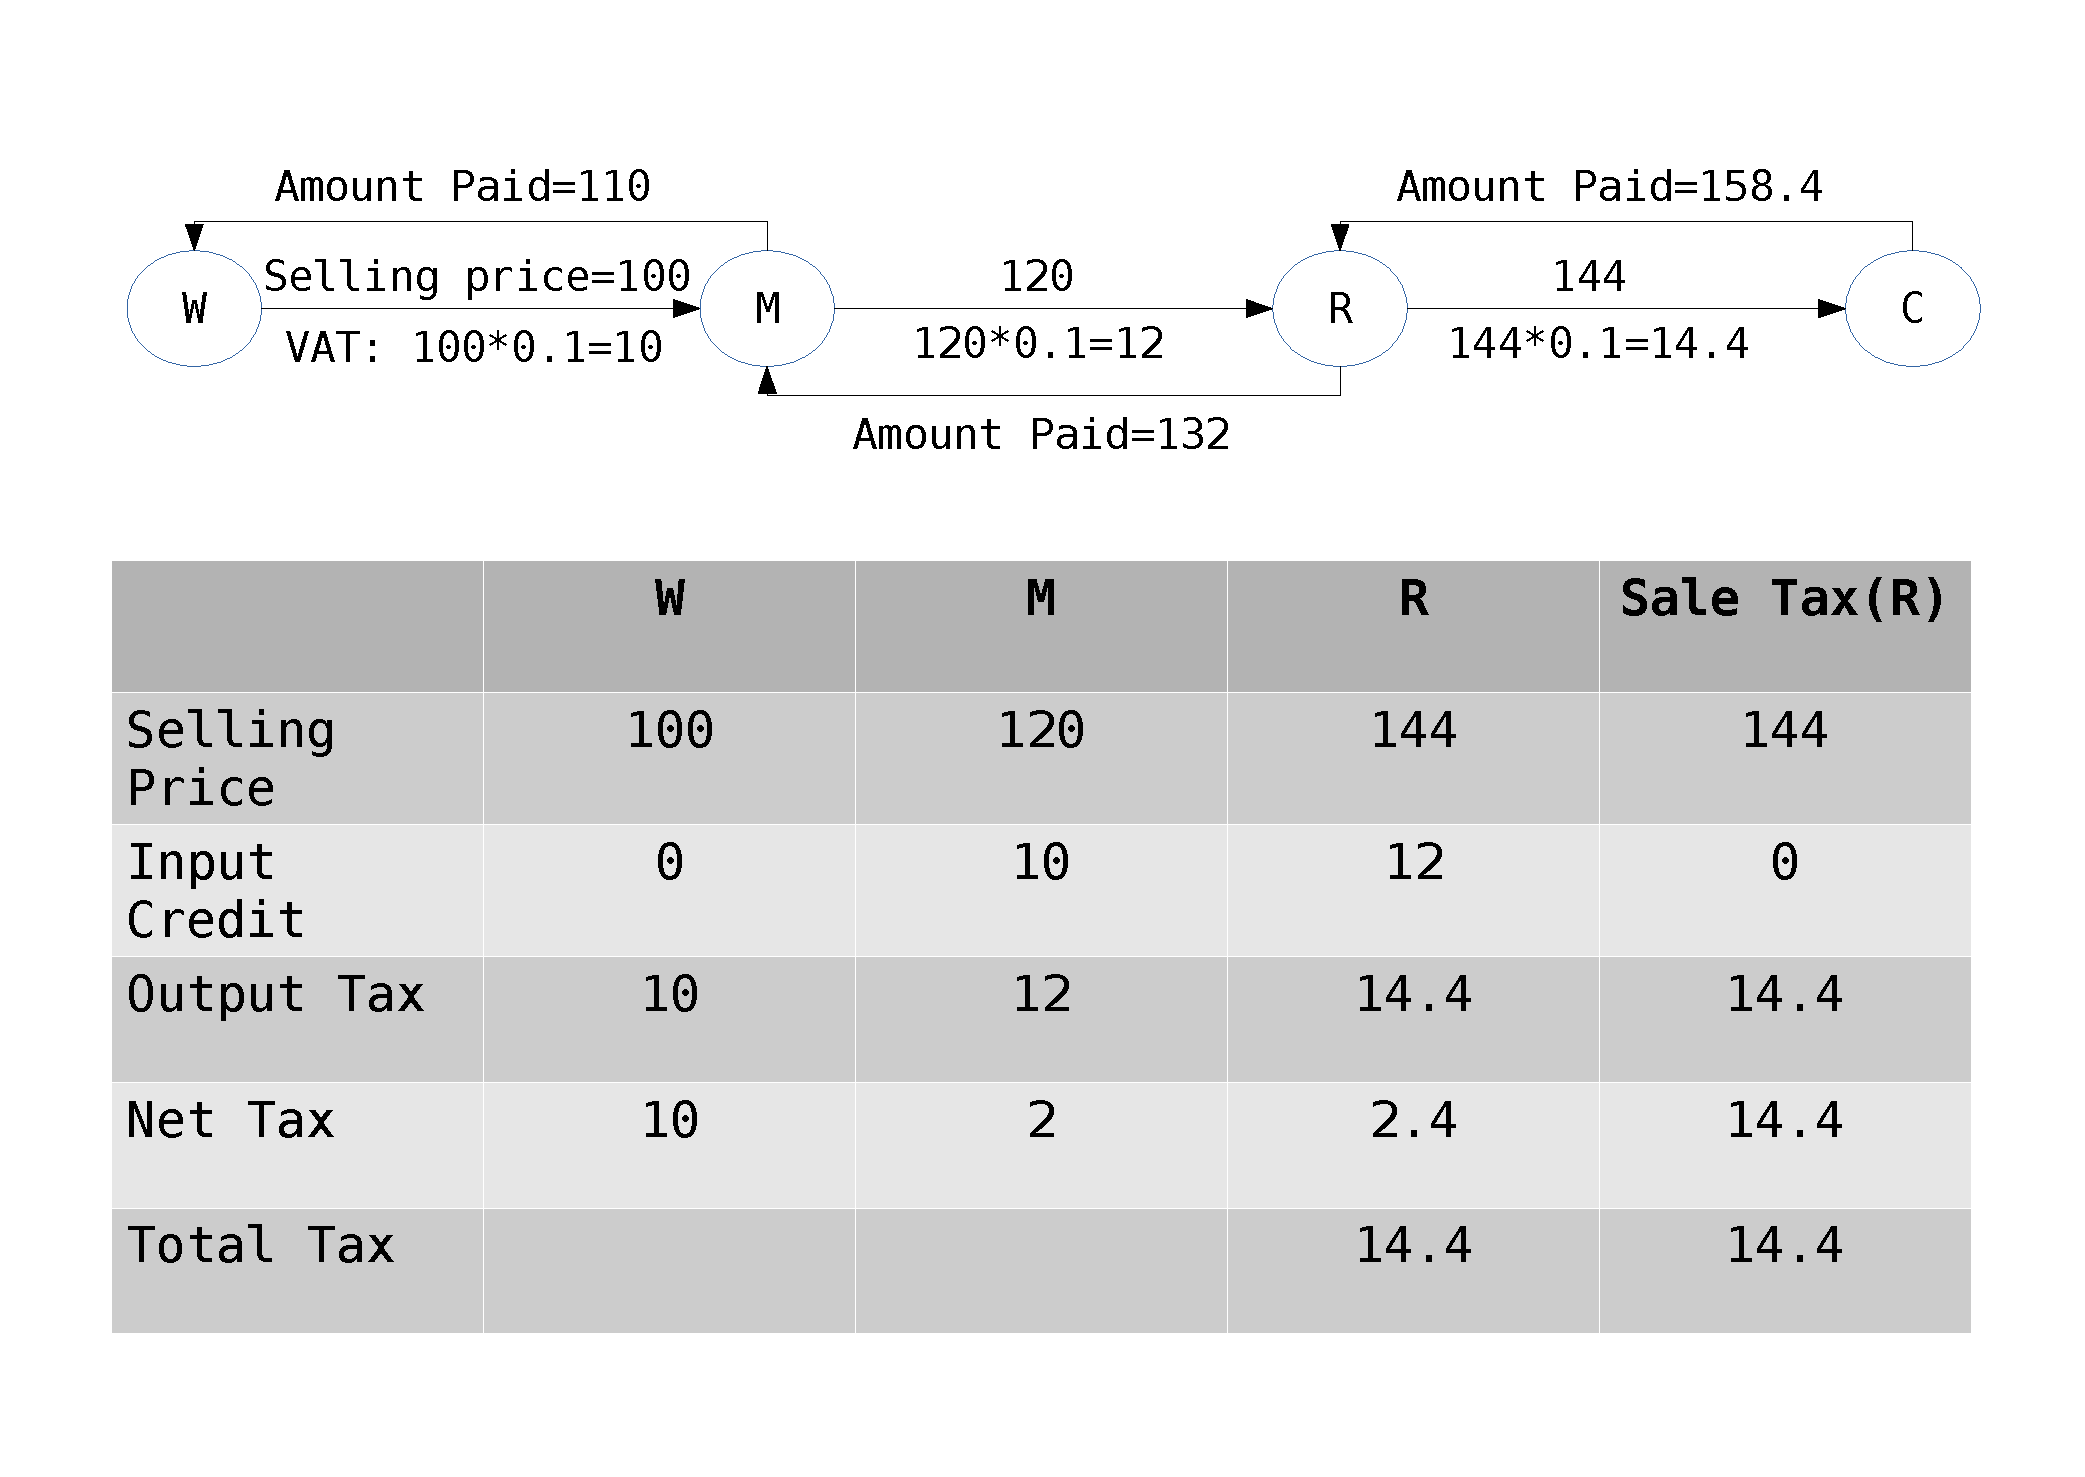
\includegraphics[width=.9\textwidth]{graphs/example_4.pdf}
\caption{Toy Model}
\label{fig:toy-model}
\floatfoot{\footnotesize An illustrative example describing how a value added tax system is different from a sales tax regime. Both the systems are revenue equivalent. In a sales tax system, the tax revenue is withheld and remitted only from the point at which sales are made to the final customer. However, in a VAT system, the tax revenue is withheld and remitted across all stages of production.}
\end{figure}

We next outline a simple example to explicate the working of the VAT to highlight features relevant for a low compliance environment. Consider a production chain as outlined in \cref{fig:toy-model} consisting of three firms and a final consumer - starting with W at the ``top'' of the chain on the left through to the final customer C at the ``end'' of the chain. Under a standard sales tax regime with ful compliance with a tax rate of 10\%, W and M do not withhold any tax. C pays \$14.4 (10\% of 144) to R as tax and R is presumed to remit the entire amount to the tax authority. Now under a
VAT regime, W withholds \$10 in tax from M (10\% of 100), M withholds \$12 in tax from R, and R will withhold \$14.4 in tax from C. Finally, W will remit \$10 to the tax authority. M, however, will declare that it has already paid \$10 as tax to M and will deduct that amount from the \$12 it withheld and will remit only \$2, and similarly, R will remit only \$2.4. The amount that should finally be deposited to the the tax authority is still \$14.4. Therefore, in a system with full compliance, the VAT system collects the same tax revenue as a standard sales tax.

There are two key points worth emphasizing here. First, M (R) gets a ``tax credit'' (also called ``input credit'') only if W (M) is registered with the tax authority. This, theoretically, should push firms which sell to registered firms to register themselves and thereby reduce informality in the system. However, in practice the effectiveness of this incentive is far from clear given the difficulties faced by developing countries in persuading firms to become formal and in monitoring the VAT system.\footnote{\cite{bird2005value}. See also \cite{DePaulaScheinkman:2010} for a model showing that such incentives can also create ``chains'' of informality.} In our study
approximately 75\% of firms make some some sales to unregistered firms.\footnote{Note we cannot distinguish between final consumers and unregistered firms in our data. However, sales to unregistered entities occur at all nodes on a VAT chain, not just at the end point.}

Second, as is standard in VAT systems, each firm has incentives to under-report sales and to over-report inputs so that a buyer and the corresponding seller have opposed incentives. For example, in the transaction between W and M, W has an incentive to not report the transaction to avoid remitting to the state any tax it has withheld while M wants to report the entire amount to maximize its tax credit. Therefore, M's incentives should act as a check on behavior of W particularly if the tax authority can credibly cross-verify M's reports with W's reports. 

If, however, M can sell to unregistered firms, then the tax authority can no longer third-party verify all of its sales. This failure of third-party verification in turn opens up the possibility of collusion between W and M.  For instance, if M sells \$ 60 worth of goods to unregistered firms (U), it can conceal this transaction completely since it cannot be verified by third-party reporting. This in turn provides M an incentive to collude with W to reduce reported purchases (so as to ensure that reported sales are not lower than reported purchases). For instance, they can agree upon a purchase amount of \$50. This reduces W's tax liability to \$5 relative to the no collusion scenario. This agreement does reduce M's input tax credit by \$5 as well. However, since M only reports half his sales, the decline in her output tax more than off-sets the decline in her input tax credit so that her overall tax liability falls (in this case by $50\%$) from \$2 to \$1.\footnote{Since M is not reporting the sale to U, it can give the tax-break to U by not collecting the tax or it can withhold the tax but not remit it. Anecdotally, we are aware of both the scenarios occurring in Delhi and we are indifferent between them.} (Refer to \cref{tbl:evasion-desc})

\begin{table}[h]
%\footnotesize
\begin{threeparttable}
\caption{Evasion in Toy Model}
\begin{tabular}{|l|l|l|l|l|l|l|l|l|c|c|}
\hline
& \multicolumn{4}{|c|}{Sales} & \multicolumn{4}{|c|}{Purchases} & \multicolumn{2}{|c|}{Tax} \\ \hline
& \multicolumn{2}{|c|}{Actual} & \multicolumn{2}{|c|}{Reported} & \multicolumn{2}{|c|}{Actual} & \multicolumn{2}{|c|}{Reported} & Actual & Reported \\ \hline
& (1) & (2) & (3) & (4) & (5) & (6) & (7) & (8) & (9) & (10) \\ \hline
& R & U & R & U & R & U & R & U & & \\ \hline
W & 100 &0 & 50 & 0 & 0 & 0 & 0 & 0 & 10&5 \\ \hline
M & 60 & 60 & 60 & 0 & 100 & 0 & 50 & 0 & 12 -10 = 2 & 6-5 = 1\\ \hline 
R & 0 & 72 & 0 & 60 & 60 & 0 & 60 & 0 & 7.2-6 = 1.2 & 6-6 = 0 \\ \hline
\end{tabular}
\begin{tablenotes}[para,flushleft]
Actual columns indicate the true values of sales or purchases. Reported columns indicate the declared values of sales or purchases. Columns (1), (3), (5), (7) show transactions with registered firms. Columns (2), (4), (6), (8) show transactions with registered firms. Tax evasion is feasible because M makes half of its sales to unregistered firms.   
\end{tablenotes}
\label{tbl:evasion-desc}
\end{threeparttable}
\end{table}


Continuing with the example as above we can consider three different scenarios depending upon whether M and R collude.  First, we assume that there is no collusion between R and M and R reports sales truth-fully. In this case, R sells output to final consumers for \$72 collecting \$7.2 in taxes of which \$6 are off-set by his input tax credit so that \$1.2 is remitted to the authority. Second, consider the case where R and M do not collude but R decides unilaterally to under-report sales to C since such sales are not subject to third-party verification. In this scenario, R can in principle report any amount of sales to C but perhaps recognizing that zero (or negative) value-added in the final step may invite further scrutiny, will report the smallest amount about \$60 he is comfortable with to the tax authority. Third, M and R have incentives to collude so that the entire transaction can be carried out without involving another party U. In particular, M and R can agree to make \$60 worth of transactions on-the-books and remaining \$60 off-the-books.

\begin{figure}[h] 
\caption{Third party verification}
\label{fig:matching_model}
\centering
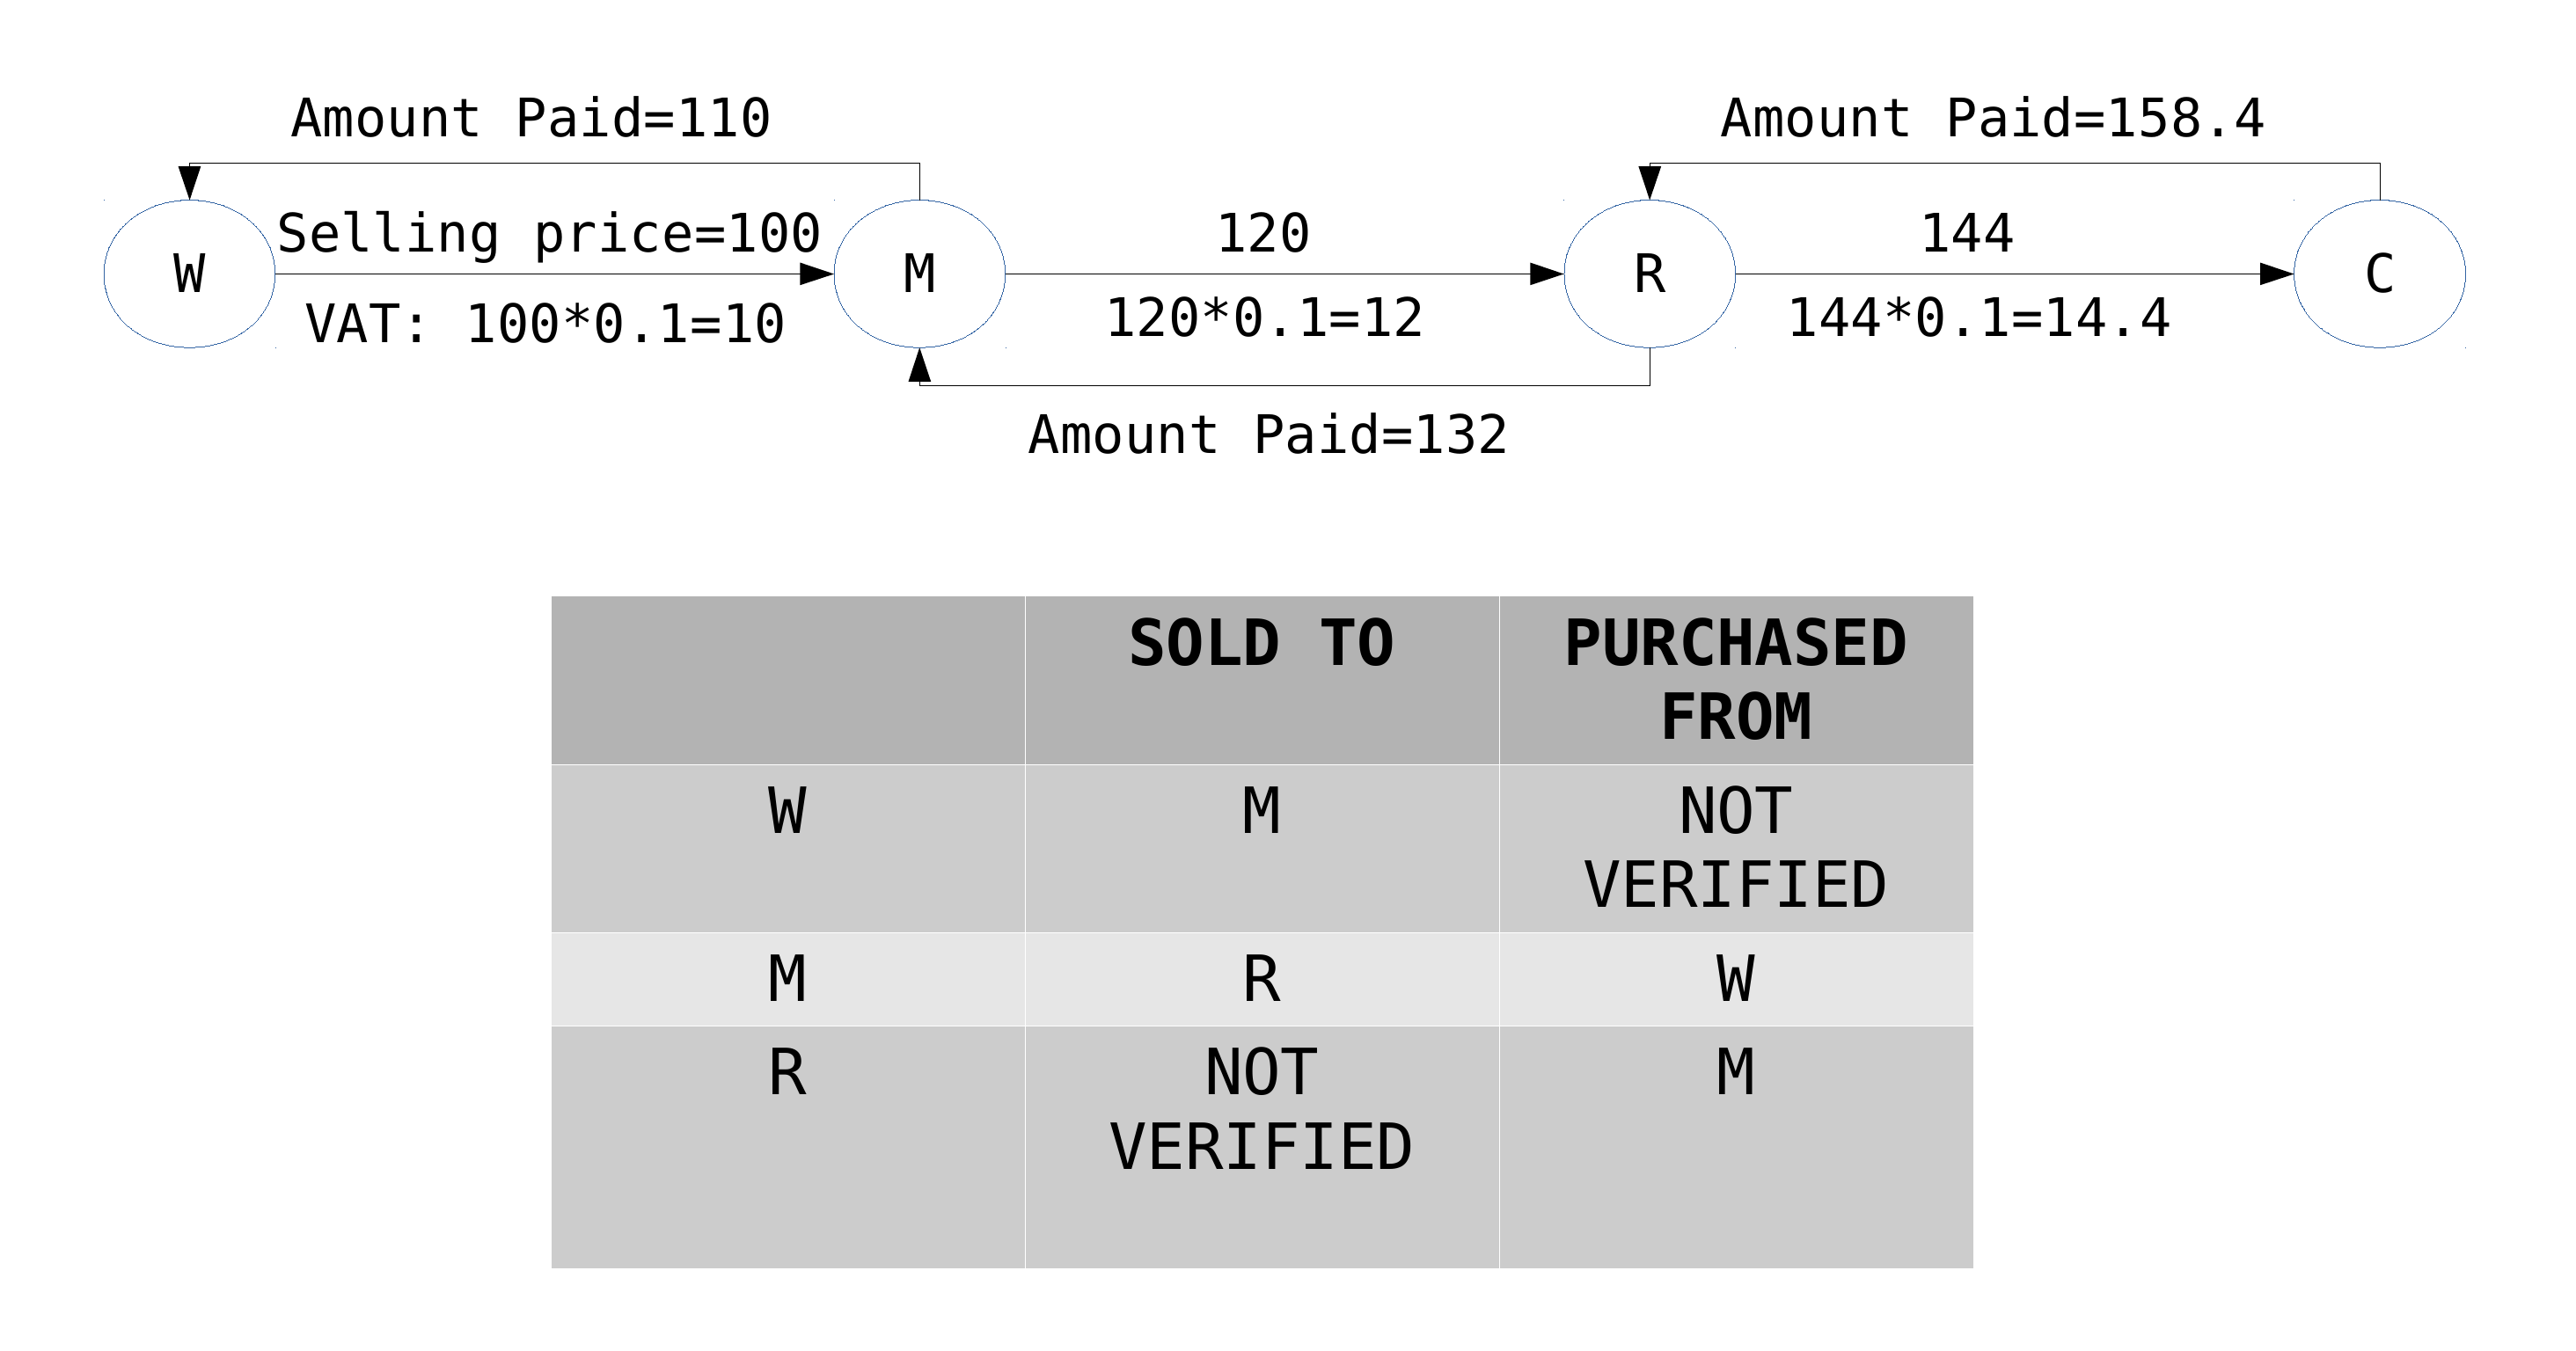
\includegraphics[width=.9\textwidth]{graphs/example_5.png}
\floatfoot{\footnotesize Description of information declared by firms. For example, W will have information about M in its SOLD TO annexure and will have no information in its PURCHASED FROM annexure. Correspondingly, M will declare information about W in its PURCHASED FROM annexure, which can be used to verify sales made by W.}
\end{figure}

The simple example above makes two points relevant for our setting. First, holding constant the probability of detection, sales to unregistered firms by a seller at any point in the chain enables pairwise collusion between the seller and his immediate supplier regardless of the presence of collusion further below (or above) the pair. This in turn implies that we can use the \cite{kleven2016can} model to analyze the implication of third-party reporting since we can limit attention to pairwise comparisons of buyers and sellers and do not need to rely on ``unraveling from the bottom'' arguments typically invoked to examine evasion in VAT systems. Second, one can reasonably interpret the pre-reform status quo within the model as the situation where no transactions had effective third-party verification and tax reports were not matched across buyers and sellers. The imposition of automated matching between buyers and sellers means that the transactions between W and M and M and R now need to be evaluated as above while the transactions between R and C are still not third-party verifiable (see \cref{fig:matching_model}). This difference across W and R firms in the effect of the policy along form the basis of our identification strategy.


\subsection{VAT in Delhi: Policy Change}
\label{background_policychange}
From Q1 of 2012-13 (year 3 of our data), firms were required to file two additional forms (known as Annexure 2A and Annexure 2B) in addition to their usual consolidated returns (which is referred to as Form 16, \cref{sec:consolidated_form}). The main change for our purposes is that the additional forms required firms to provide transaction details (i.e. sales and purchase information) disaggregated at the firm and tax-rate level for all registered firms and that the authority began to cross-check buyer and seller reports automatically on its own server.\footnote{Different commodities are taxed at different rates. Firm A reporting transactions with Firm B would group together all transactions for commodities taxed at the same rate into a single transaction report.}

Annexure 2B recorded all firm sales in the past tax period disaggregated at the registered buyer level for each tax rate. Annexure 2A recorded purchases  disaggregated at the seller level for each tax rate (refer to \cref{sec:annexure_form}). All firm level entries in Forms 2A and 2B had to include the tax IDs of all registered firms involved in the transaction thus enabling the tax authority to easily cross-check reports. The only across firm aggregation that was permissible was for unregistered firms (i.e. firms with no tax identification numbers which includes final consumers). The new forms meant that for the first time the tax authority could cross-check buyer and seller reports (for dis-aggregated transactions) from the submitted returns alone (i.e. without having to resort to an audit).\footnote{Recall that before the policy change (from 2005-2012) firms did not have to provide firm-level reports of purchases or sales but instead were only required to report total sales aggregated across all firms and correspondingly total purchases aggregated across all registered firms (and the corresponding purchase amount from unregistered firms). They were required to maintain firm-level information for their own records in case of an audit - though based on the audit notice data that we have, probability of getting audited is extremely low (less than 1\%).}

\section{Data}
\label{sec:data}
We have detailed tax data from the government of New Delhi for 5 years (from 2010 to 2015) which we describe in detail below.

\subsection{VAT Returns}
\label{subsec:data-returns}
We have anonymized VAT returns for the entire universe of registered firms for 5 years - 2010-11 (Y1), 2011-12 (Y2), 2012-13 (Y3), 2013-14 (Y4), 2014-15 (Y5). Each firm is assigned a unique identifying number so we can follow a firm over time as well as track its presence in other firms' returns (from Y3 onwards). However, anonymization implies
that we cannot link the firms to any other publicly available information on the firms.

We have detailed information on the line items in the consolidated returns (form 16) throughout the study period, and after quarter 1 of 2012-13, we have line items of form 2A and form 2B (refer to \cref{sec:consolidated_form} for details). For the purposes of this paper, we use the following information from form 16:

\begin{enumerate}
\item Total turnover (sales) disaggregated by destination - (i) local (within state) sales and (ii) inter-state or international sales. Local sales are taxable and can include sales to registered firms (which are third-party verifiable) and sales to unregistered firms (which are not third-party verifiable). However, the tax forms do not require firms to differentiate between the two. After quarter 1 of 2012-13, we can use information in form 2A and form 2B to construct our own measures to categorize the sales, but form 16 does not explicitly ask for this information.
\item Total tax withheld by the firm from local sales - this is referred to as the output tax liability. This is a tax liability and needs to be deposited with the tax authority after the requisite adjustments -- viz. the deduction of input credits, see below.
\item Total purchases disaggregated by destination - (i) local (within state) purchases and (ii) inter-state or international purchases. Local purchases are decomposed into purchases to registered firms (which are third-party verifiable) and purchases from unregistered firms (which are not third-party verifiable). Only local purchases from registered firms are eligible for input tax credits.
\todo[inline, caption={Question from AM}]{Q: Do we ever do DID on interstate outcomes? Ans: We did and no change}
\item Total tax paid by the firm on local purchases from registered  firms - this is referred to as input credit. Input credit is subtracted from the firms' output tax liability when computing the tax the firm needs to remit to the tax authority.
\item For the three post-reform years (Y3, Y4, Y5) we also have quarterly information on sales and purchases from forms 2A and 2B as described earlier (\cref{sec:annexure_form}).  For each quarter and each tax-rate, sales made by a firm are disaggregated at the (registered) firm and tax-rate level, and likewise purchases are disaggregated at the (registered) firm and tax-rate level. Therefore, for each firm, items (1)-(4) are available at the firm quarter and tax rate level.
\item Finally, the total tax remitted by the firm to the tax authority.
\end{enumerate}

Items (1)-(4) above are further broken down by tax-rates (since different goods are taxed at different rates) and we also observe some additional information such as penalties, past tax credits and liabilities. 

\subsection{Firm Characteristics}
\label{subsec:data-dp}
In addition to tax return information we also have basic information provided by the firm at the time of registration. We observe the date of registration, the revenue ward (i.e. the broad, largely, geographic
categorization of the firm for revenue purposes), the nature of business (e.g. manufacturer, wholesaler, retail trader, exporter, importer), the legal status of the business (e.g. proprietorship, private limited company, public sector undertaking, government corporation) as well as the other tax schemes and acts the firm is
subject to (e.g. the central excise act, service tax) and whether a firms is registered for international trade (import or export).
\todo[inline, color=green, caption={Question from AM}]{Can we use this extra information to better classify some of the retailers}

\subsection{Audit Notices}
\label{subsec:data-audit}
We have information (for Y4 and Y5) audit notices sent out by the tax authority. These dated notices identify the targeted firm and are usually the first step in a sometimes lengthy audit procedure. We use this information to quantify the extent to which the tax authority checks on problematic returns.

\subsection{Sample}
\label{subsec:sample}
We limit our analysis to firms present throughout the period of study. This sub-sample comprises 85\% of all firms present in year 1 and 95\% of all tax revenues in year 1. Thus, the sample consists of the near universe of revenue generating firms (see \cref{fig:vatdeposited-all} and \cref{fig:vatdeposited-alwayspresent}). We do not, therefore, address the effect of the policy on firm registration and exit decisions. We restrict our primary sub-sample further to firms that are exclusively wholesalers or retailers as reported on their VAT registration forms.\footnote{Given the previous selection rule this means we are  restricting ourselves to firms registered in or before 2010-11.} These comprise 27\% of all firms present in year 1 and 44\% of all tax revenues in year 1.\footnote{In terms of year 5, these firms comprise 19\% of the sample but still contribute 43\% of the tax revenues.} However, we use larger sub-samples for some specifications which we describe in greater detail in section \ref{sec:results}. In addition, we also provide additional data description in \cref{sec:overall_analysis}.

\todo[inline,caption={Firm Exit},color=green]{We Should Look at Firm Exit in our sample at Some Point.}  

\section{Empirical Strategy}
\label{sec:empirical_strategy}
We adopt a quasi-experimental approach to examine the effectiveness of the increased information available to the tax authority.

\subsection{Identification: Wholesalers vs Retailers Over Time}
\label{subsec:identification}
Relative to wholesale firms, retail firms are more likely to sell to final consumers and conversely wholesalers are more likely to sell to registered firms.\footnote{Verified in \cref{fig:salesregistered}.} As pointed out earlier, the change in filing requirements should therefore affect the two differentially. Following the reform, the tax authority can easily cross-check wholesaler sales to registered firms whereas previously this would only occur via an extensive and time-consuming audit process. On the other hand, sales made by retailers (any firm in general) to final consumers remain unaffected by the policy change. Finally, purchases by both types of firms from registered firms should be affected equally. This argument suggests then that if wholesalers find it harder to understate sales, then we should expect the policy to lead to an increase in taxes remitted by wholesalers driven by an increase in output tax declarations.\footnote{See also the discussion in \cref{sec:conceptual} which links to the relevant theoretical literature.}

Our identification strategy is thus a difference-in-difference approach comparing the difference in trends between wholesalers and retailers before and and after the policy reform. The key identifying assumptions are that the timing of the third-party verification policy introduction is exogenous for our outcomes of interest and that in the absence of the reform, the (counterfactual) evolution of outcomes among wholesalers would evolve just as the (observed) evolution of outcomes among retailers (the "parallel trends" assumption). The multiple years of data before and after the reform allows us to look at the evolution of outcomes over relatively long time periods, see \cref{sec:eventstudy-analysis}.

\subsection{Model Specification}
\label{subsec:identification_model}
The main outcome variable is the amount of VAT remitted. However, as is typical in these settings the dispersion in tax remitted is quite large (refer to \cref{fig:lorenzyear1}).\footnote{Others e.g. \citet{pomeranz2015no} finds similar dispersion for VAT returns.} Further, a large number of firms (roughly 49\%) remit zero VAT. This implies that the mean may not be a representative measure of central tendency and mean regression estimates may be sensitive to outliers. We address this concern by using alternative outcome variables and estimation methods (in addition to using standard mean regressions). Specifically, we look at linear probability model using as an outcome an indicator variable equal to one if the VAT deposited is larger than zero (for the extensive margin results). In addition, we also use quantile regressions and tobit type models (although incorporating fixed-effects for a large set of firms is a computational challenge for both methods) and also estimate linear regression models over sub-samples defined by membership in deciles of relevant firm-characteristics.

\todo[inline,caption={Need to do Quantile Regressions},color=green]{We need to implement quantile regressions with fixed effects at some point.}{ }

Our basic specification is
\begin{equation}\label{eq:basic}
y_{it}=\alpha_i+\nu_t+\beta*\text{Post}_{it}+\gamma*\text{Post}_{it}*\mathbb{I}\{\text{Wholesaler}_{i}\}+\epsilon_{it}
\end{equation}

$\text{Post}_{it}$ is equal to 1 if the observation for firm $i$ comes from the post-policy period -- years 3--5 for the annual analysis and quarters 9--20 for the quarterly analysis since the policy was introduced between years 2 and 3 and quarters 8 and 9 -- and zero otherwise. $\text{Wholesaler}_{i}$ is a dummy variable equal to 1 if firm $i$ self-reports as being a wholesaler and 0 if the firm self-reports as a retailer. The $\nu_{t}$ are a full set of time dummies and $\alpha_{i}$ are firm fixed-effects. The main outcome variables of interest are (a) an indicator for whether the firm remitted any positive amount of VAT, and (b) the amount of VAT remitted. To dig deeper into whether the effect of the policy is coming from the input side (i.e. by reducing input credits) or from the output side (i.e. by increasing the output tax liability) we
also estimate regressions using (c) input credit claimed and (d) total output tax liability as outcomes. We also construct a new outcome variable which is the difference between output tax liability and input tax credits. This allows our outcome variable to be negative and takes care of the concerns arising out of there being a mass point at
zero. All the outcome variables have been inflation adjusted to the corresponding baseline price levels i.e. outcome variables for the annual analysis have been indexed at the 2010 level, and outcome variables for the quarterly analysis have been indexed at the Q1-2010 level. 

The parameter of interest is $\gamma$ which captures the differential effect of the policy on wholesalers relative to retailers. Under the maintained "parallel-trends" assumption, for which we provide supportive evidence below, $\gamma$ is consistently estimable using standard fixed-effect methods. We also present more flexible specifications that allow for time-varying differences in group means both before and after the policy reform. In particular, we include time-dummies for each period and also interaction between each time-dummy and a wholesaler dummy. Concretely,

\begin{equation}\label{eq:flex}
y_{it}=\alpha_i+\nu_t+\gamma_t*\nu_t*\mathbb{I}\{\text{Wholesaler}_{i}\}+\epsilon_{it}
\end{equation}

Where, in addition to the firm-fixed effects $\alpha_i$ and the set of time-dummies (represented here in the interest of brevity and clarity by $\nu_t$ here), we now include a full set of time-dummies interacted with the wholesaler dummy (represented here as $\nu_t*\mathbb{I}\{\text{Wholesaler}_i\}$). The coefficients $\{\gamma_s\}_{s \in S }$\footnote{S denotes the set of post-policy time periods.} are the parameters of interest and are intended to capture the differential effect of the policy on wholesalers (relative to retailers) in period s relative to the period immediately prior to the policy's introduction. Finally, in all analysis standard errors are clustered at the firm level. In \cref{subsec:falsification-test} we present additional robustness in quarterly results by adding $\text{Pre}_{it}$ dummy which is equal to 1 for tax quarters 7 and 8 i.e. just before the introduction of the policy.

\section{Results}
\label{sec:results}

\subsection{Description: Wholesalers vs Retailers}	
\label{subsec:descripton_treatment_control}
Our main sample comprises of 32,979 retailers and 19,515 wholesalers who file a return during the entire period of our study.\footnote{This is when returns are aggregated to the annual level. We discuss the sample size when we consider quarterly frequency regressions in \cref{sec:quarterlyresults}.} Pre-policy means in year 1 along with changes in means over the pre-policy period for the two groups are shown in \cref{tbl:group1_summary_real}. In general, wholesalers are considerably larger than retailers; we provide additional data description in \cref{sec:overall_analysis} and discuss evidence of parallel trends in \cref{subsubsec:evidence-parallel-trends}.

\begin{table}[h]
\footnotesize  
%\scriptsize  
\begin{threeparttable}
\caption{Summary Statistics: Retailer and Wholesaler Sample (Real terms)}
\begin{tabular}{lHccHcc} \hline \hline
 &&(1)&(2)&&(3)&(4)\\
Variables & &Retailers & Diff & & Wholesalers & Diff  \\ \hline
\% Positive VAT Deposited Firms & 32979 & 0.59 & -0.00 & 19515 & 0.53 & -0.00\\
&&(0.00)&(0.00)&&(0.00)& (0.00)\\
VAT Deposited & 32979 & 0.64 & 0.02 & 19515 & 1.31 & -0.01\\
&&(0.06)&(0.02)&&(0.20)& (0.05)\\
Total Turnover & 32979 & 24.27 & 2.23 & 19515 & 80.80 & 4.70\\
&&(1.31)&(0.74)&&(6.47)& (2.59)\\
Turnover (Local) & 32979 & 18.43 & 1.89 & 19515 & 49.72 & 4.66 \\
&&(1.18)&(0.68)&&(4.45)& (1.23) \\
Credit Claimed & 32979 & 0.95 & 0.10 & 19515 & 1.41 & 0.23 \\
&&(0.04)&(0.01)&&(0.24)& (0.08)\\
Output Tax & 32979 & 1.53 & 0.12 & 19515 & 2.63 & 0.22\\
&&(0.08)&(0.02)&&(0.41)& (0.07) \\
Tax Remitted/TotalTurnover & 32028 & 0.01 & -0.00 & 18994 & 0.01 & -0.00 \\
&&(0.00)&(0.00)&&(0.00)& (0.00)\\
Credit/TotalTurnover & 32028 & 0.11 & -0.07 & 18994 & 0.07 & -0.04\\
&&(0.04)&(0.04)&&(0.03)&(0.03) \\
Output Tax/TotalTurnover & 32028 & 0.05& 0.00 & 18994 & 0.03 & 0.00\\ 
&&(0.00)&(0.00)&&(0.00)& (0.00)\\
Nonlocal Turnover/TotalTurnover & 32028 & 0.25 &0.00& 18994 & 0.37& -0.00\\ 
&&(0.00)&(0.00)&&(0.00)&(0.00) \\ \hline \hline
\end{tabular}
\begin{tablenotes}[para,flushleft]
Summary statistics for selected variables in Year 1. Amounts are in million rupees, with \rupee 65 approximately equal to \$1. $N_W=32979$, $N_R=19515$. 951 wholesalers and 521 retailers report zero turnover. Column (2) and Column (4) report mean differences between real values of  year 2 and year 1. Values have been price adjusted in year 1 terms. Standard error in parenthesis. 
\end{tablenotes}
\label{tbl:group1_summary_real}
\end{threeparttable}
\end{table}

As mentioned earlier, these two groups account for a substantial part of VAT collections. In year 1, both groups remitted 44\% (\rupee 46.7 billion) of total VAT collections and the corresponding number is 43\% for the last year of the study. In total, they account for 55.5\% of the increase in the VAT collections from the sample of firms present in each of the 5 years. \Cref{fig:group1-pretrends} and \cref{fig:group1-pretrends-quarterly} show the trends of VAT remitted at the annual as well as the quarterly level for the two groups (along with point-wise 95\% confidence intervals).


\begin{figure}[h] 
\caption{Wholesalers vs Retailers: Annual trends (in real terms) with confidence intervals}
\label{fig:group1-pretrends}
\centering
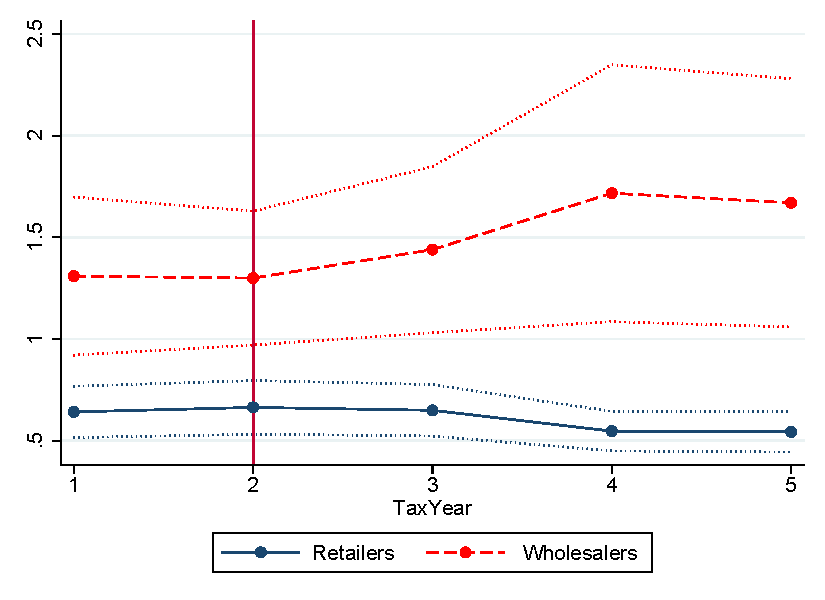
\includegraphics[width=.9\textwidth]{graphs/MeanMoneyDeposited_annual_with_confidenceintervals_Real.pdf}
\floatfoot{\footnotesize $N_W=19515, N_R=32979$. Average VAT remitted is in million rupees, inflation adjusted to 2010-11 price levels, with \rupee 65 approximately equal to \$1. Pointwise 95\% CI included. Third party verification started in year 3.}
\end{figure}


\subsubsection{Supporting Evidence for the Parallel Trends Assumption}
\label{subsubsec:evidence-parallel-trends}
We begin by providing some evidence that changes in the outcome variables of interest were evolving similarly among wholesalers and retailers in the periods prior to the reform. We  examine the key outcome variable, tax remitted by firms. \Cref{fig:group1-pretrends} presents group-wise means for tax remitted in each period and \cref{fig:eventstudy-figure-annual}(a) graphs the coefficients for the difference between the two groups in each period from estimating \cref{eq:flex}. We cannot reject the null hypothesis that the changes in tax remitted during the first two periods were the same across wholesalers and retailers (p-value=0.61). We also carry out the same analysis at the quarterly level (\Cref{fig:group1-pretrends-quarterly,fig:eventstudy-figure-quarter}(a)) which yields the same conclusions.\footnote{In \cref{subsec:eventstudy-econometrics} we describe the formal statistical tests for testing the absence of differential pre-trends in more detail.} 

This gives us some confidence that the key (untestable) assumption of parallel trends may be reasonable when examining tax remits. We also carry out the same analysis for the other outcomes of interest: (a) Output Tax, (b) Input Credit, (c) the Difference between the two and (d) whether any VAT was remitted. In all cases we cannot reject the null that the changes in outcomes in the pre-policy period were similar between the two groups.

\subsection{Results: Difference in Difference}
\label{subsec:diffindiff}
\Cref{fig:group1-pretrends,fig:eventstudy-figure-annual}(a) also suggest that wholesaler tax remits increased post-policy while retailer remits remained more or less unchanged. The regressions below formally confirm these conclusions. We begin by examining changes on the ``extensive'' margin -- changes in whether a firm remits any tax with the tax authority -- before examining changes in the amount remitted. We then examine the effect of the policy on the two key constituents of a firm's tax obligation --- input credit and output tax liability.

\Cref{tbl:group1-levels} shows the results of the difference-in-difference regressions at the firm-annual level. In column (1) the outcome is a dummy variable for whether the firm remits any tax. The proportion of wholesaler firms depositing any tax goes down by a statistically significant 2\%, though this is a relatively modest decrease of 4\% from a baseline of 53\%. Next, VAT remitted (column 2) increases by a substantively (and statistically) significant \rupee 0.38m for wholesale firms. This is an increase of 29\% over a year 1 mean of \rupee 1.31m. The wholesalers response is particularly notable since it is in start contrast to the retailer response -- for retailers total tax remitted actually decreases post-policy. These result are consistent with the conceptual framework outlined in \cref{sec:conceptual}. Wholesalers who have higher third-party verifiable income and interact with more registered firms respond much more to the improvement in third-party verification relative to retailers.

\begin{table}[h]
\footnotesize
\scalebox{0.9}{
\begin{threeparttable}
\caption{Diff-in-Diff: Wholesalers and Retailers (Annual)}
\begin{tabular}{lcHcccc} \hline
  \hline
 & (1) & (2) & (2) & (3) & (4) & (5)\\
  VARIABLES & Positive VAT  & VAT Remitted$>$ & VAT Remitted & Tax Credit & Output Tax & Output Tax -\\
   & Remitted Firms & Previous Year &  &  & & Input Credit \\ \hline
Post*Wholesaler & -0.02*** & -0.02*** & 0.38*** & -0.12 & 0.25** & 0.37*** \\
 & (0.00) & (0.01) & (0.14) & (0.15) & (0.11) & (0.14) \\
Post & 0.04*** & 0.03*** & -0.09* & 0.18*** & 0.09** & -0.09** \\
 & (0.00) & (0.00) & (0.05) & (0.05) & (0.04) & (0.05) \\\hline
Mean Dep.Var. &.53 & & 1.31 & 1.41 & 2.63& 1.22 \\
&(.00)&&(.20)&(.24)& (.41)&(0.20)\\ \hline
Observations & 262,470 & 209,976 & 262,470 & 262,470 & 262,470& 262,470\\
R-squared & 0.63 & 0.33 & 0.89 & 0.83 & 0.97 & 0.89 \\ \hline
Number of Firms & 52,494 & 52,494 & 52,494 & 52,494 & 52,494 & 52,494\\ \hline \hline
\end{tabular}
\begin{tablenotes}[para,flushleft]
Robust standard errors in parentheses, clustered at firm level. $N_W=19515,N_R=32979$. Monetary amounts are in million rupees, with \rupee 65 approximately equal to \$1. All monetary amounts have been inflation indexed to 2010-11 price levels. Column (1) shows linear probability regressions of the probability of depositing a positive amount. Column (2)-(4) respectively show regression of the mean VAT remitted by firms, input credit claimed by firms, and output tax collected by firms. To address the concern that VAT deposited has a significant mass at zero, Column(5) shows regression of the difference between output tax and input credit declared by firms.  Mean Dep. Var. shows the mean and standard errors for wholesaler firms in year 1. *** p$<$0.01, ** p$<$0.05, * p$<$0.1.
\end{tablenotes}
\label{tbl:group1-levels}
\end{threeparttable}}
\end{table}

We next examine the proximate causes of the changes in tax remitted by examining changes in output tax liability and input tax credit respectively. Consistent with the arguments in \cref{sec:conceptual} we see that there is a substantive increase in the output tax liability for wholesalers relative to retailers -- a 9.5\% increase from year one. Further, we see that input credits decline for wholesalers relative to retailers though the estimate is not significant at conventional levels. Overall, the signs of the wholesaler response along each component dimension are then consistent with the predictions of the framework outlined in \cref{sec:conceptual}. Retailer behavior is somewhat harder to rationalize. A rise in input credits is consistent with increased collusion (to minimize tax liability) or an accurate measure of purchases if under-reporting purchases is harder post-reform (recall retailers who under-report sales will have an incentive to also under-report purchases to avoid having value added estimates that are suspiciously low). We also see an increase in output tax liability for retailers post-policy and this is somewhat unexpected, particularly since retailers make most of their sales to unregistered firms. We explore this further in the next section when we examine heterogeneity in returns. Column (5) examines the difference between  output tax liability and input credits and is consistent with the argument that retailers are able to offset increases in output tax liability by matching increases in input credits (as in e.g. \cite{Carrilloetal:2017}) while wholesale firms are unable to do so.\footnote{The reason Col (5) is not the same as Col (2) is because some firms have negative tax liability and hence remit no tax.} Finally, we note that the asymmetry between effects on input credits and output tax liability suggests that that effects on wholesalers cannot be easily ascribed to a differential growth account. 
\todo[inline,caption={Comment from AM}, color=green]{What if the policy led to changes in the fraction of firms overall that were registered or unregistered. then this could just reflect fact that a firms buyers became registered post-policy}

As a robustness check, \cref{tbl:event-falsification-table} repeats the regressions whose results are presented in \cref{tbl:group1-levels} but at the quarterly frequency.\footnote{The sample is now reduced to 11,482 wholesalers and 15,337 retailers, as firms with less than \rupee 5 million in turnover only had to submit returns annually or semi-annually in the first two years of our data.} The results are consistent with the results described at the annual frequency and so we do not discuss them here. Moreover, as described earlier, we carry out event falsification test by looking at coefficients on $\text{Pre}_{it}*\mathbb{I}\{\text{Wholesaler}_{i}\}$ where $\text{Pre}_{it}$ is 1 if tax-quarter is 7 or 8 i.e. just before the introduction of the policy. We find that pre-policy effect on wholesalers is close to zero, precisely estimated, and statistically significant.\footnote{More details in \cref{subsec:falsification-test}.}

\todo[inline, caption={Question from AM}]{Don't we normalize period 8 coefficient to be zero? Ans: This is a different specification}

\begin{figure}[h] 
\centering
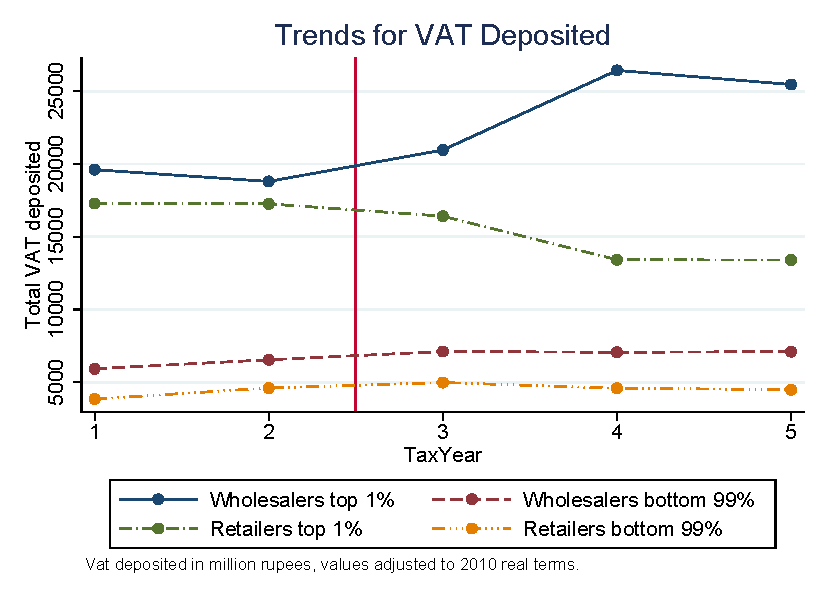
\includegraphics{graphs/MoneyDepositedTrendsTopPercentilePanel_Annual_Real.pdf}
\caption{Tax Remitted by top percentile and bottom 99\% of firms}
\label{fig:money-onepercentile}
\floatfoot{\footnotesize Notes: This figure plots the total VAT remitted by the panel of top 1\% and the bottom 99\%, in terms of VAT remitted in year 1, of wholesalers and retailers. $N_W=19515,N_R=32979$. Therefore, top 1\% of retailers are 329 firms and top 1\% of wholesalers are 195 firms. Rest of the firms form bottom 99\%. Monetary amounts are in million rupees, inflation adjusted to 2010-11 price levels, with \rupee 65 approximately equal to \$1.}
\end{figure}

\subsubsection{Heterogeneity}
\label{subsubsec:diffindiff_heterogeneity}
We next turn to exploring heterogeneity in our estimates. There are two main reasons for this. First, as we saw in the previous table, there is a significant point mass at zero for tax remitted. This suggests that exploring alternatives to mean regressions may be a useful exercise. Further, \cref{tbl:group1-levels} indicates that while the policy had limited extensive margin effects (i.e. on whether firms remit any tax) there were substantive intensive margin effects, suggesting the the policy may have affected different wholesalers differently.


\begin{table}[h]
\footnotesize
\scalebox{0.9}{
\begin{threeparttable}
\caption{Diff-in-Diff: Wholesalers and Retailers (Annual, Real Terms, Top Percentile)}
\begin{tabular}{llHllll} \hline
  \hline
 & (1) & (2) & (2) & (3) & (4) & (5)\\
  VARIABLES & Positive VAT  & VAT Remitted$>$ & VAT Remitted & Input Credit & Output Tax & Output Tax -\\
   & Remitted Firms & Previous Year &  &  & & Input Credit \\ \hline
Post*Wholesaler & 0.02* & 0.06 & 34.75** & -15.94 & 19.96** & 35.90** \\
 & (0.01) & (0.06) & (13.62) & (13.38) & (8.89) & (14.06) \\
Post & -0.02** & -0.07* & -12.02** & 9.31** & -3.47 & -12.78*** \\
& (0.01) & (0.04) & (4.68) & (4.07) & (3.65) & (4.46) \\ \hline
Mean Dep.Var. &1 & & 100.59 & 36.27 & 138.29& 102.02 \\
&(0.00)&&(18.55)&(23.42)& (39.17)&(18.39)\\ \hline
Observations & 2,620 & 2,096 & 2,620 & 2,620 & 2,620 & 2,620 \\
R-squared & 0.42 & 0.38 & 0.88 & 0.84 & 0.98 & 0.88 \\
Number of Firms & 524 & 524 & 524 & 524 & 524 & 524\\ \hline \hline
\end{tabular}
\begin{tablenotes}[para,flushleft]
Robust standard errors in parentheses, clustered at firm level. $N_W=195,N_R=329$. Monetary amounts are in million rupees, inflation adjusted to annual 2010-11 price levels, with \rupee 65 approximately equal to \$1. Column (1) shows linear probability regressions of the probability of remitting a positive amount. Column (2)-(4) respectively show regression of the mean VAT remitted by firms, input tax credit claimed by firms, and output tax collected by firms. To address the concern that VAT remitted has a significant mass at zero, Column(5) shows regression of the difference between output tax and input credit declared by firms.  Mean Dep. Var. shows the mean and standard errors for top 1\% wholesaler firms in year 1. *** p$<$0.01, ** p$<$0.05, * p$<$0.1
\end{tablenotes}
\label{tbl:group1-toppercentile}
\end{threeparttable}}
\end{table}

We begin by examining the evolution of tax remitted for different sub-groups of wholesalers and retailers. In particular, we partition each group into two sub-groups ranked according to tax remitted in the first year of the study -- the top 1\% and the remaining 99\%.\footnote{We use tax remitted as the stratifying variable because it is also the variable used by the authority to determine firms that will be examined by the special ward in charge of large tax-payers.} The results are graphed in \cref{fig:money-onepercentile}; two points are worth noting. First, tax remits remain relatively stable for the bottom 99\% of wholesale firms as compared to the top 1\%. In contrast, tax remits for retail firms as a whole (both in the 1\% as well as in the 99\% sub-groups) are relatively stable throughout the study period. This analysis suggests that it is worthwhile to examine heterogeneity in treatment effects across different percentiles of the baseline outcome distribution.\footnote{A natural estimation method here would be to use quantile regressions. We are currently working on implementing a stable quantile regression model with fixed effects on our data.} In \cref{tbl:group1-toppercentile,tbl:group1-bottom99} we present the regression adjusted comparisons of \cref{fig:money-onepercentile}. There are at least three points of interest. First, the policy has no differential effects on wholesalers relative to retailers in the bottom 99\% sub-sample. Second, the response of the top 1\% of wholesalers is sharply different from that of the top retailers. For the top retailers, input credits increase and output tax declines modestly\footnote{The output tax response is not statistically significant at conventional levels.} so that overall tax remits fall by $22.9\%$ (relative to a top 1\% retailer baseline of \rupee 52.55m) after the policy. In stark contrast, input credits decline and output tax liability increases for wholesalers (relative to top retailers) so that post-policy overall tax deposited rises by $34\%$ (relative to the baseline mean).

\begin{table}[h]
\footnotesize
\scalebox{0.9}{
\begin{threeparttable}
\caption{Diff-in-Diff: Wholesalers and Retailers (Annual, Real Terms, Bottom 99 Percentile)}
\begin{tabular}{llHllll} \hline
  \hline
 & (1) & (2) & (2) & (3) & (4) & (5)\\
  VARIABLES & Positive VAT  & VAT Remitted$>$ & VAT Remitted & Input Credit & Output Tax & Output Tax -\\
   & Remitted Firms & Previous Year &  &  & & Input Credit \\ \hline
Post*Wholesaler & -0.02*** & -0.02*** & 0.03 & 0.04 & 0.05 & 0.02 \\
 & (0.00) & (0.01) & (0.03) & (0.06) & (0.07) & (0.02) \\
Post & 0.04*** & 0.03*** & 0.03*** & 0.09*** & 0.13*** & 0.03*** \\
 & (0.00) & (0.00) & (0.01) & (0.02) & (0.02) & (0.01) \\
\hline
Mean Dep.Var. &0.53 & & 0.31 & 1.06 & 1.26& 0.20 \\
&(0.00)&&(0.01)&(0.06)& (0.06)&(0.02)\\ \hline
Observations & 259,850 & 207,880 & 259,850 & 259,850 & 259,850 & 259,850 \\
R-squared & 0.63 & 0.33 & 0.58 & 0.78 & 0.78 & 0.82 \\
Number of Firms & 51,970 & 51,970 & 51,970 & 51,970 & 51,970 & 51,970\\ \hline \hline
\end{tabular}
\begin{tablenotes}[para,flushleft]
Robust standard errors in parentheses, clustered at firm level. $N_W=19,320,N_R=32,650$. Monetary amounts are in million rupees, inflation  adjusted to 2010-11 price levels, with \rupee 65 approximately equal to \$1. Column (1) shows linear probability regressions of the probability of remitting a positive amount. Column (2)-(4) respectively show regression of the mean VAT remitted by firms, input tax credit claimed by firms, and output tax collected by firms. To address the concern that VAT remitted has a significant mass at zero, Column(5) shows regression of the difference between output tax and input credit declared by firms.  Mean Dep. Var. shows the mean and standard errors for wholesaler firms in year 1. *** p$<$0.01, ** p$<$0.05, * p$<$0.1
\end{tablenotes}
\label{tbl:group1-bottom99}
\end{threeparttable}}
\end{table}

\begin{figure}[h] 
\centering
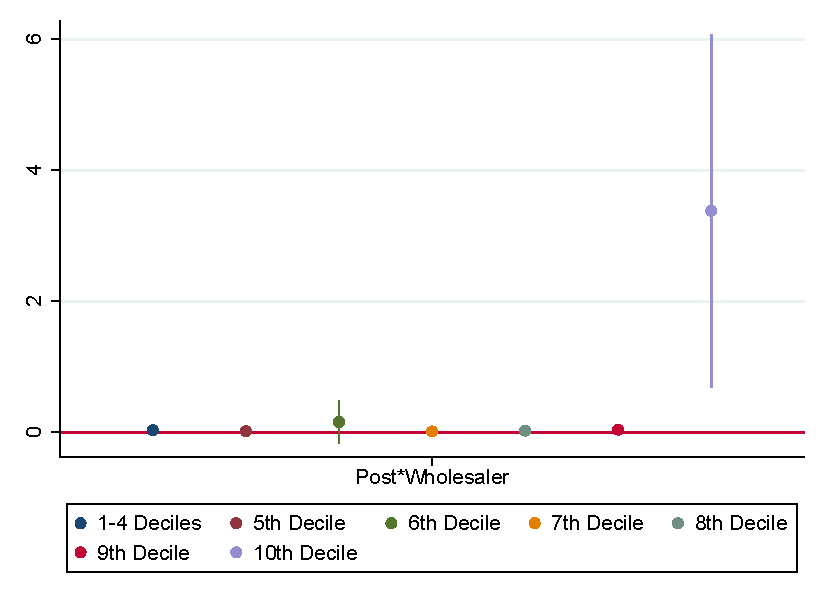
\includegraphics[width=.8\textwidth]{graphs/HeterogeneityMoneyDeposited_Real.pdf}
\floatfoot{\footnotesize Notes: This figure plots the difference between wholesalers and retailers for different deciles, based on VAT remitted in the first year. The x axis indicates the decile. Confidence intervals at the 95\% level. $N_W=32979$,$N_R=19515$. Coefficients are in million rupees, inflation adjusted to 2010-11 price levels, with \rupee 65 approximately equal to \$1.The first group consists of 4 deciles because all the firms in that group do not remit any VAT.}
\caption{Heterogeneity Analysis: VAT Remitted for Wholesalers vs Retailers}
\label{fig:heterogeneity-figure-annual-vatdeposited}
\end{figure}
These results confirm the differential effects of the policy and also help us better understand firm responses. First, the opposing signs and differences in magnitudes and significance of the output tax response between top wholesalers and retailers is consistent with the hypothesis that top wholesalers are more constrained in their responses.\footnote{As pointed out earlier a differential growth story for top wholesalers is less plausible since input credit and output tax respond in opposite directions while increased growth via sales would be more likely to be reflected in increased purchases as well.} Further, top wholesalers are both more likely to be monitored by a special tax assessment unit and have more third-party verifiable income. In contrast, top retailers are less likely to be monitored by the special unit and also have much less third-party verifiable income. The lack of any differential response among the bottom 99\% of wholesalers (relative to retailers) in turn suggests that differences in third-party verifiable income alone (without commensurate monitoring) are not sufficient for generating greater collections. These
differential effects therefore provide some sobering evidence on the effectiveness of the VAT at increasing collections in low compliance environments.\footnote{\cite{almunia2017analysis} find substantial discrepancies in third-party reports in Uganda and also emphasize the limited enforcement capacity of the state as an important constraint. In our context, discrepancies are less of a concern post-policy, because of automatic matching, relative to collusion.} Second, retailers (both large and small) increase input credits claimed after the policy while the wholesaler response is either much more muted or even negative. These results are consistent with the retailers relatively higher ability to collude with a smaller number of input supplies.
%Further, less than 5\% of the bottom 99\% of wholesalers (and $\textbf{??}$ of the bottom 99\% of retailers) are monitored by the special assessment unit.
 %(on average retailers in our sample purchased from \textbf{??} registered firms while the corresponding figure is \textbf{??} for wholesale firms)

\todo[inline,caption={SM: Numbers Needed}]{We need some numbers for the two paragrahps above. the sentences have been commented out for now. DO NOT DELETE. I am also not sure how many registered firms our wholesalers purchase from. It is not clear that this point above even makes any sense unless the numbers line up as predicted.}

\todo[inline,caption={Shekhar Size Definition Question},color=green]{SM: I though we defined size by turnover in the baseline year. That seems to be the most acceptable definition no? Also, can we check that the footnote where we use turnover gives us similar results. I know we looked at it at some point.}

\begin{figure}[h] 
\centering
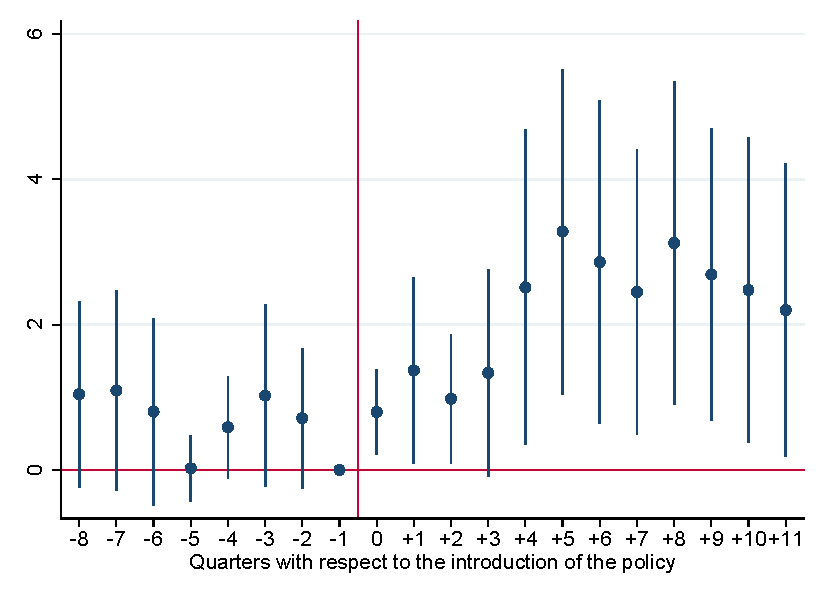
\includegraphics[width=.8\textwidth]{graphs/EventStudy-MoneyDeposited-Quarter_TopDecile_Real.pdf}
\floatfoot{\footnotesize Notes: Graphical event-study analysis of the effect of third party verification policy on wholesalers compared to retailers. Limiting the set of wholesalers and retailers to the top 10\% of each group in terms of VAT remitted in quarter 1. Confidence intervals were constructed with heteroskedasticity-robust standard errors, clustered at the firm level. The coefficient for the wholesale group in the quarter (-1) prior the policy is normalized to zero. The regressions include firm fixed  effects and time effects. The x axis indicates time, with quarterly observations and zero indicates the first year of the third party verification policy. We have 20 quarters of data from 2010-11 to  2014-15. Confidence intervals at the 95\% level. $N_W=1148$,$N_R=1533$. Coefficients are in million rupees, with inflation adjusted to Q1 2010-11 price levels, with \rupee 65 approximately equal to \$1. Pretrends are not statistically significant.}
\caption{Top Decile: VAT Remitted for Wholesalers vs Retailers}
\label{fig:eventstudy-figure-quarter-vatdeposited-topdecile}
\end{figure}

As an alternative approach we estimate \cref{eq:basic} separately for different deciles based on the baseline (year one) distribution of tax remitted.\footnote{We constructed deciles using group-specific distributions of tax remitted in year one.} \Cref{fig:heterogeneity-figure-annual-vatdeposited} plots the coefficient of interest ($\gamma$ from eq. \ref{eq:basic}) from each of the seven separate regressions though we present regression results only from the regressions using the top decile subsample in \cref{tbl:group1-decile}.\footnote{The remaining regression results are omitted for brevity and are available upon request.} \Cref{fig:eventstudy-figure-quarter-vatdeposited-topdecile} shows the event-study plots for the top decile of wholesalers and retailers on VAT remitted as an outcome variable. Other outcome variables are shown in \cref{fig:eventstudy-figure-quarter-topdecile}.

The figures and table are consistent with the earlier graph. The treatment effect is only substantively significant for the top decile, and is relatively negligible for all other deciles. Tax remitted by wholesalers in the top decile goes up by \rupee 3.38m, a 26.7\% increase over the \rupee 12.6m remitted in year one. Given the relative stability of retailer outcomes across deciles, the results imply that it is only the biggest wholesalers that are driving the large increase in tax remitted in the mean regressions in \cref{tbl:group1-levels}.

There are at least two possible reasons for the differential effects on the largest wholesalers. First, 96\% of the top 1\% of wholesalers in our sub-sample are assessed by a special tax unit (known as the Key Customers Services Unit) that is tasked with collections form large firms (the corresponding figure for the top 1\% of retailers is 80\%) and which has greater resources for inspection and other activities.\footnote{See \cite{DasGuptaetal:2004} for a discussion of similar units in the context of personal income tax in India.} Second, as we show below, the ease of third-party verification had a much larger effect on the top 1\% of wholesalers (relative to other wholesalers and retailers) since the bulk of their sales were to other registered firms. The combination of these two factors is consistent with the results in the table above. We are currently seeking more information on the special ward assigned for larger firms.

\todo[inline, caption={Do better analysis on KCS}, color=green]{Revenue and administrative efficacy of KCS. Do whatever you can think of.}

\begin{table}[h]
\footnotesize
\begin{threeparttable}
\caption{Diff-in-Diff for Top Decile: Wholesalers and Retailers (Annual, Real Terms)}
\begin{tabular}{lcHcccc} \hline \hline
  & (1) & (2) & (2) & (3) & (4) & (5) \\
 VARIABLES & Positive VAT  & VAT Remitted$>$ & VAT Deposited & Tax Credit & Output Tax & Output Tax -\\
 & Remitted Firms & Previous Year &  &  & & Input Credit \\ \hline
 Post*Wholesaler & 0.02*** & 0.04** & 3.38** & -1.77 & 1.68 & 3.46** \\
 & (0.01) & (0.02) & (1.38) & (1.43) & (1.04) & (1.42) \\
Post & -0.06*** & 0.01 & -1.11** & 1.00** & -0.21 & -1.20*** \\
 & (0.00) & (0.01) & (0.47) & (0.42) & (0.39) & (0.45) \\ \hline
Mean Dep.Var. &1 & & 12.65 & 6.98 & 19.73& 12.75  \\
&(.00)&&(1.97)&(2.40)& (4.04)&(1.95) \\ \hline
Observations & 26,240 & 20,992 & 26,240 & 26,240 & 26,240 & 26,240 \\
R-squared & 0.41 & 0.28 & 0.89 & 0.84 & 0.97 & 0.89 \\
Number of Firms & 5,248 & 5,248 & 5,248 & 5,248 & 5,248 & 5,248 \\ \hline \hline
\end{tabular}
\begin{tablenotes}[para,flushleft]
\Cref{eq:basic} results of the effect of third party verification policy on wholesalers compared to retailers. Limiting the set of wholesalers and retailers to the top 10\% of each group in terms of VAT remitted in year 1. Robust standard errors in parentheses, clustered at firm level. Number of wholesalers is 1951 and number of retailers is 3297. Monetary amounts are in million rupees, inflation adjusted to 2010-11 price levels, with \rupee 65 approximately equal to \$1. Column (1) shows linear probability regressions of the probability of remitting a positive amount of VAT. Column (2)-(4) respectively show regression of the mean VAT remitted by firms, of the input tax credit claimed by firms, and the output tax collected by firms. *** p$<$0.01, ** p$<$0.05, * p$<$0.1.
\end{tablenotes}
\label{tbl:group1-decile}
\end{threeparttable}
\end{table}

\section{Mechanism}\label{sec:mechanisms}
% \citet{dufloplumber} in her 2017 Ely lecture at the AEA has highlighted the importance of economists getting into the plumbing details of a policy. In this section we show some evidence which sheds light on how the policy was actually executed on the ground. 
% ;
\begin{figure}[h] 
%\centering
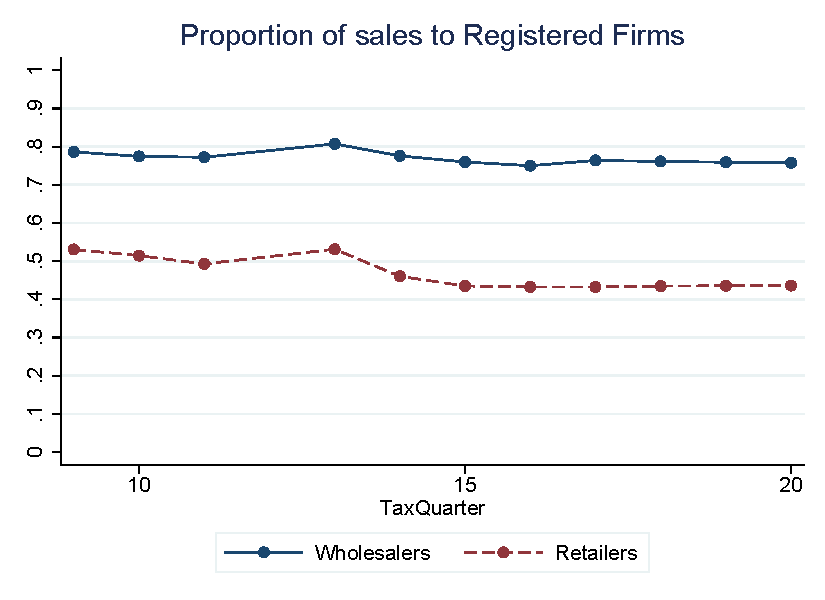
\includegraphics{graphs/ProportionSalesRegistered.pdf}
\caption{Sales to registered firms}
\floatfoot{\footnotesize Proportion of total sales made to registered firms for wholesale and retail firms.}
\label{fig:salesregistered}
\end{figure}

In this section we explore potential mechanisms for the reduced form results above. Specifically, we examine the pattern of sales made to registered firms and how it evolved over time. This is important because the conceptual framework outlined in \cref{sec:conceptual} highlighted the role of third-party verifiable transactions as a moving force and in our context only interactions with registered firms are third-party verifiable.\footnote{We explore other a few other implementation details that shed light on how the policy was actually executed on the ground in \cref{sec:execution}.}

%We begin by examining the pattern of sales made to registered firms and how it evolved over time
\subsection{Sales to Registered Firms}
\label{subsec:registered_sales}
\Cref{fig:salesregistered} displays quarterly sales to registered firms as a proportion of total sales separately for wholesalers and retailers. The graph is only from quarter 9 (year 3) onwards because in the pre-policy period firms were only required to report a total sales amount without further disaggregation. The lack of a complete series on this variable also limits its use as a direct measure of formality which could be used to examine heterogeneity (although we do present some suggestive evidence below). In addition, changes along the extensive margin for interacting firms also complicates the interpretation (e.g. if the policy led to more firms becoming registered). Over the entire post-policy period wholesale firms made approximately 78\% of their sales to registered firms while the corresponding figure for retail firms is 43\%.

\begin{figure}[h] 
\centering
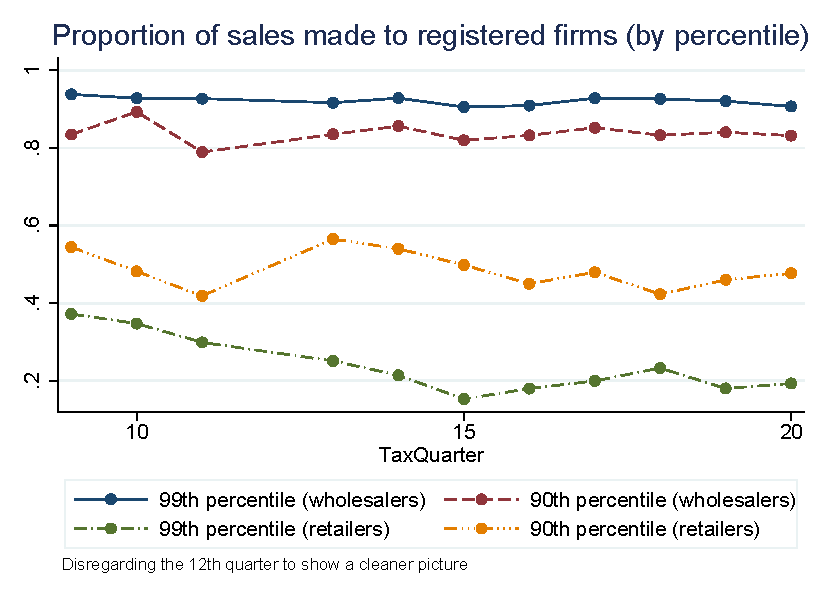
\includegraphics{graphs/ProportionSalesRegisteredTopPercentile_v2_without12.pdf}
\caption{Sales to registered firms}
\floatfoot{Describing the proportion of sales made to registered
  firms. Comparing the declarations by top percentile of wholesalers
  and retailers with the 90th percentile.}
\label{fig:sales_registered_percentile}
\end{figure}

We next examine this proportion for the $99^{th}$ and $90^{th}$ percentile for each group in \cref{fig:sales_registered_percentile}. There are three points worth noting: First, over 90\% of total sales are made to registered firms by the top percentile of wholesale firms (and the figure is similar, though somewhat lower for the $90^{th}$ percentile). Second, a significant proportion of sales by exclusively retail firms are made to registered firms. This is \emph{prima facie} surprising and we discuss its interpretation below. Finally, the proportion of total sales made to registered firms is lower ($\approx 20\%$) among the top percentile of retail firms compared to the $90^{th}$ percentile ($\approx 50\%$), suggesting that smaller retailers are more likely to sell to registered firms.


There are at least four potential reasons for the retailer related findings. First, a larger retailer may in turn sell to smaller (registered) retailers. This could explain the results for the top percentile of retailers but would not suffice for explaining why smaller retailers make \emph{more} sales to registered firms than
larger retailers.

A second possibility is that at least some of the reported sales to registered firms by retailers are in fact fraudulent -- that they are created to provide fraudulent input credits and hence reduce tax collections.\footnote{A simple example is the following: retailer A declares a proportion of her sales to final customers as in fact having been made to firm B. Firm A's tax obligation does not change relative to the counter-factual where all sales are reported as sales to final customers. On the other hand, Firm B reduces his tax liability so that, after accounting for the probability of detection, there is an incentive for both parties to conclude the transaction and for B to make a side payment to A.} We are exploring this possibility in ongoing work and in particular using network analysis to examine further the characteristics of registered firms who make purchases from small retailers.

%\textbf{Another simple explanation could be that retailers indeed avoid declaring a significant portion of their sales to final customers and as a result the declared proportion of sales to registered firms increases mechanically. Lastly, we should not rule out that selling significantly to registered firms is a feature of retailers as well and this is the first time we have had empirical evidence to discuss it.}

A third explanation is that greater under-reporting of sales to unregistered firms by smaller retailers (relative to larger retailers) leads mechanically to smaller retailers reporting a higher fraction of sales to registered firms relative to larger retailers. Finally, the data may be an accurate record of retailer behavior rather than a reflection of any evasion. At the moment
we do not have enough information to distinguish between these competing explanations though we are pursuing further work here as well.

We directly examine the relationship between the proportion of sales to registered firms and the change in tax collections as a result of the policy change. We conduct a triple-difference comparison by comparing the difference between wholesalers and retailers with a higher fraction of sales to registered firms to the corresponding difference between firms with a lower fraction of sales and finally doing these comparisons before and after the policy reform for the the third difference. Specifically,
\begin{multline}\label{eq:ddd}
y_{it}=\alpha_i+\nu_t+\beta*\text{Post}_{it}+
\delta*\text{Post}_{it}*\text{PropRegistered}_i\\+ \gamma*\text{Post}_{it}*\mathbb{I}\{\text{Wholesaler}_{i}\}+\lambda*\text{Post}_{it}*\mathbb{I}\{\text{Wholesaler}_{i}\}*\text{PropRegistered}_i+\epsilon_{it}
\end{multline}

In \cref{eq:ddd}, in addition to what we have already described for \cref{eq:basic}, we now also add a variable called $\text{PropRegistered}_i$ which is the proportion of sales declared to be made in quarter 9 (the first quarter immediately after the introduction of the policy). Now the coefficient of interest is $\lambda$ which tells us the effect of the policy on wholesaler firms which make greater proportion of their sales to registered firms. Another coefficient of interest is $\delta$ which shows the effect on retailers. 

\begin{table}[h]
\footnotesize
\caption{Triple Difference: Wholesalers/Retailers; Before/After;Sales
  to Registered Firms in real terms}
\scalebox{0.95}{
\begin{threeparttable}
\begin{tabular}{llllll} \hline
& (1) & (2) & (3) & (4) & (5) \\
VARIABLES & Positive VAT & VAT Remitted & Input Credit & Output Tax & Output Tax \\ 
&Remitted & & & & - Input Credit \\ \hline
Post*Wholesaler*Registered Sales & 0.02** & 0.17** & -0.04 & 0.12* & 0.16** \\
 & (0.01) & (0.07) & (0.07) & (0.06) & (0.08) \\
Post*Wholesaler & -0.02*** & 0.06** & -0.01 & 0.05** & 0.07*** \\
 & (0.00) & (0.02) & (0.02) & (0.03) & (0.02) \\
Post*Registered Sales & 0.01 & 0.02 & 0.02 & 0.04** & 0.03 \\
 & (0.01) & (0.02) & (0.02) & (0.02) & (0.02) \\
Post & 0.01** & -0.07** & 0.03 & -0.04 & -0.07** \\
 & (0.00) & (0.04) & (0.03) & (0.04) & (0.03) \\ 
  \hline
Observations & 536,380 & 536,380 & 536,380 & 536,380 & 536,380 \\
 R-squared & 0.55 & 0.86 & 0.78 & 0.96 & 0.86 \\ 
 Number of Firms & 26,819 & 26,819 & 26,819 & 26,819 & 26,819 \\ \hline \hline
\end{tabular}
\begin{tablenotes}[para,flushleft]
\footnotesize Regressions run at the quarterly level on the set of  firms that file returns in all quarters. $N_{W}=11482$,$N_{R}=15337$). All regressions include time dummies and firm fixed-effects. Column (1) displays results from a linear probability model where the outcome is a dummy for any VAT remitted. The outcomes in Column (2)-(4) are VAT remitted, input credit claimed and output tax collected. The outcome in column (5) is the difference between output tax and input credit (as one method to deal with the point mass at zero in the VAT remitted outcome). Monetary amounts are in million rupees, inflation adjusted to 2010-11 price levels, with \rupee 65 approximately equal to \$1. Robust standard errors in parentheses, clustered at the firm level. *** p$<$0.01, ** p$<$0.05, * p$<$0.1.
\end{tablenotes}
\label{tbl:group1-diff-in-diff-in-diff}
\end{threeparttable}}
\end{table}

The central weakness with this strategy is that, as pointed out earlier, we can construct sales to registered firms separately from
total sales only in the post-policy period. In the pre-policy phase firms were only required to report total sales (which was the basis of their output tax liability). We use the fraction of sales made to registered firms in the first post-policy quarter (quarter 9) as our measure of sales to registered firms -- and hence our static measure of third-party verifiable income at the start of the policy. 

The results in \cref{tbl:group1-diff-in-diff-in-diff} show that the treatment effect of the automation policy is stronger for wholesale firms who sell more to registered firms. Somewhat surprisingly, retailers with a larger fraction of sales to registered firms do not see any differential increases in tax remitted (or tax credits or output tax liability). This finding is again consistent with the first three explanations and high sales to registered firms is definitely not a feature of the actual transactions that retailers carry out.

\section{Conclusion} 
\label{sec:conclusion} 
In this paper we evaluate the effect of a policy reform that implemented a key pillar of the VAT system -- increasing the tax authority's ability to easily cross-check buyer and seller reports against each other. Under the previous regime such cross-checks could only be carried by instituting a rare, lengthy and expensive audit process. We interpret this change in policy as one that increased the number of transactions that were effectively third-party verifiable by the tax authority. We evaluate the effect of this policy change in the Indian state of Delhi -- a low compliance environment with a large number of
transactions being made to unregistered firms (i.e firms that do not file returns with the tax authority) -- to shed light on the effectiveness of third-party verification in an emerging economy.

We evaluate the effect of the policy by comparing two groups of firms likely to be differentially affected by it - wholesalers and retailers. In particular, wholesalers are more likely to sell to registered firms relative to retailers. We hypothesize that requiring transacting firm tax identifiers in returns should affect wholesalers more than retailers.  Further, given the invoice-credit structure of the VAT systems in India, we expected that the primary wholesaler response would be through increases in output tax liability.

Our results confirm these hypotheses with wholesalers increasing tax remits by \rupee 0.38 million (an increase of 29\% relative to the pre-policy period) driven by increases in output tax liability. We further find that increases in tax remits are concentrated among the very largest wholesale firms, with the top 1\% of firms accounting for 89.3\% of the increase in tax remitted.  Next, we note that 96\% of wholesale firms in the top 1\% are under the jurisdiction of a special unit of the tax authority which focuses exclusively on high tax revenue firms (the corresponding figure for retail firms is 80\%). Our results suggest that information and monitoring are complements in that we see the strongest effect of improved third-party verification from firms that are more likely to interact with other registered firms and are more closely monitored by the tax authority. These results suggest a more nuanced picture of the state's capacity to tax and the effectiveness of third-party verification in low compliance environments.


% findings are consistent with the
% hypothesis that the tax authority uses its new cross-checking capacity
% to differentially target large firms and is doing so at least somewhat
% effectively.
\todo[inline,caption={Shekhar: Origin of 1\% Number}, color=green]{I don't see  this 89.3\% increase in the earlier discussions}


%We also document the importance of the details of policy execution, which is especially relevant when the enforcement and execution capacity is weak. First, we show that a loophole that allowed firms to enter mutually inconsistent data appears to have been used by firms to minimize their tax obligations. Second, we see that the average number of tax form revisions increases sharply after the policy.  Third, we find that the matching of purchases and sales ex-post is around 90\%. We also find that retailers declare a significant proportion (roughly 43\%) of their sales to registered firms. At the very least, all this can be considered as evidence of increased compliance costs for firms or alternatively as evidence of collusion.

% The data also allows us to ask other questions. In future work we
% intend to investigate how did the special tax teams affect the tax
% collections differently from wholesalers compared to retailer or more
% generally try to better understand how the state's tax capacity
% interacts with improved information in other dimensions.
% ;
\todo[inline,caption={To Dos},color=green]{
Move all figures and tables to the appendix -- I think we should definitely do this. It's the norm for most applied work and I like being able to flip directly to the end to look at tables and figures unlike now when I have to keep flipping pages. \textbf{I think we said we wouldn't do this for now.}}

\pagebreak


%\begin{figure}[p] 
%\centering
%\includegraphics{graphs/TaxCreditComparison_allfirms.pdf}
%\caption{Consolidated vs transactional data}
%\floatfoot{In the first year, transaction data was not matched with the consolidated returns. Firms were clearly fudging, which was fixed in the subsequent years}
%\label{consolidated_transaction}
%\end{figure}


 


\chapter{Who is Bogus? Using One-Sided Labels to Identify Fraudulent Firms from Tax Returns}
\section{Introduction}
\label{sec:2-introduction}
Machine learning (ML) models have been effective at automating various tasks traditionally performed by humans such as character recognition, image classification, sentiment analysis, translation, and fraud detection. For many of these tasks the dataset is not constructed explicitly to provide a training set but has been re-purposed for the ML application. Such datasets may suffer from several challenges: human error in labeling (noisy labels); the labeled set could be not representative of the population (selective labels); and importantly for our application, it could record the labels of only one class (one-sided labels). For example, re-purposing a dataset that documents only criminal convictions (not all trials): the cases tried could be biased (selective labels), and it could also be unknown which cases were tried but did not end in convictions (one-sided labels). In this paper we provide solutions to some of these problems, and others, such as multiple time-period data and in-sample prediction. We do this by developing an important application on a real-world dataset: finding fraudulent firms in the Delhi value added tax (VAT) system.

VAT implementation in many low compliance environments is plagued by firms lowering their tax liability by generating false paper trails. This demand for false paper trails has led to the creation of fraudulent firms that sell fake receipts to genuine firms. These firms are referred to as ``bogus'' firms or ``bill traders'' by the tax authorities. A tax authority usually determines the existence of bogus firms by first filtering down based on a few preliminary indicators, and then undertaking physical inspections that verify if a firm is bogus or legitimate (``legit'' for short). Given the authority's limited resources these inspections are only done sporadically.  While the true revenue implication of bogus firms is unknown, our conversations with tax officials in Delhi (India) suggest that it might be considerable (\$300 million in Delhi alone is a commonly mentioned figure). A key challenge in improving tax compliance then is to regularly, cheaply and reliably identify such fraudulent firms. 

In this paper, we implement and evaluate an ML algorithm on the universe of tax returns data from the Delhi tax authority to identify such bogus firms. The classifier predicts the likelihood of a firm being bogus by using a training dataset comprising the universe of tax returns (over 3 years) and of results from past physical inspections of firms conducted by the tax officials. To our knowledge, this is the first paper to systematically study and identify these fraudulent firms in an economy with weak compliance.

We overcome several non-standard facets of the data and of our problem. First, our dataset was not constructed for the purpose of labeling for an algorithm and is, therefore, not a representative sample of the population. In our case, a small fraction of all firms are inspected, those suspected by the tax authority, and so there is a problem of selective labels \cite{lakkaraju2017selective}. On top of that, the tax authority only records bogus firms that were inspected, caught and canceled, but not firms that were inspected and found to be legitimate. Therefore, we are unable to distinguish between firms that were inspected and found to be legitimate and firms that were never inspected. We refer to this problem as that of one-sided labels, since no firm can be definitively labeled as legitimate (see \cref{fig:onesidedlabel}). The unlabeled firms are (at least weakly) less likely to be bogus than those labeled bogus, and we leverage this difference in class distribution to train a classifier. Moreover, the authority has never identified all the bogus firms in the stock of existing VAT firms, so we want to predict the labels of all unlabeled firms. Therefore, a standard classification approach with a training set and out-of-sample prediction is not viable. We employ a form of cross-validation to use the entire dataset as a training set and make predictions on all firms in the dataset not known to be bogus.

\begin{figure}[h]
  \includegraphics[width=.9\textwidth, page=5]{graphs/StylizedExample_New2.pdf}
  \caption{One sided labels}
  \label{fig:onesidedlabel}
  \floatfoot{\footnotesize Inspection is based on the tax authority's discretion and so are biased (selective labels). Class labels are known only for firms both inspected and found to be bogus, not for the rest (one-sided labels). We use all data for training, but want to predict for those firms still unlabeled.}  
\end{figure}

Second, standard evaluation methods rely on a labeled test set that does not exist in our one-sided labels context. In such a scenario, the task in which the problem is embedded can provide relevant metrics to evaluate the effectiveness of classification methods. In our case, the tax authority has limited resources for inspection and so it will be able to act on only the top model
recommendations. Therefore, it is reasonable to focus on the success of our top recommendations. While considering the performance evaluation results it is important to keep in mind that, according to tax officials, bogus firms are relatively rare (i.e. the class bogus is rare in the population).\footnote{In future work, by  closely documenting the inspection results, we intend to verify this claim.} Our performance estimates remain  valid regardless of the actual prevalence of bogus firms.

Third, in order to compare our algorithm's performance to the status quo of manual targeting for inspection, we carry out what we call point-in-time simulation. We estimate not only whether our model successfully predicts bogus firms, but also whether it would have done better than the tax inspectors themselves. To do this, we test our model's success at a point in time within the span of our dataset. We roll back the data to the state of knowledge at that time and generate predictions. We then measure the performance by using more recent data. In this manner, we can estimate the number of bogus firms our algorithm would have detected before the tax inspectors. We calculate the revenue lost to tax evasion over the period between when our algorithm could have targeted these firms and when they were actually targeted and inspected - potential revenue which we estimate at several billions of rupees (tens of millions of USD).

Finally, each firm files its returns quarterly and so supplies many data points, but its class (bogus or legitimate) is timeless. Therefore, there are several identically-formatted data points for each object of classification (the firm) and classification must be made at the object level. We train a single-period model and aggregate its predictions to the firm level. We call this approach multiple time-period prediction.

The key contributions of our work are:
\begin{compactitem}
\item A novel solution to the classification problem with one-sided  labels, where the labels of many data points are unknown and there  are definite examples only of one class.
\item Point-in-time simulation approach for evaluating real-world prediction systems. We evaluate the impact of our predictions by
  calculating how much our algorithm would have increased collections by identifying bogus firms sooner than the tax authority.
\item An approach for multiple time period (or multiple data-points) prediction, where several data points of similar format exist for each object of classification, but prediction is made at the object  level.
\item An application of machine learning on a large dataset for an emerging economy government to address an important policy problem. Our results indicate that by using our tool the tax administration can prevent fraud up to \rupee1-3 billion (\$15-45 million).
\item A proposed mechanism through which bogus firms may operate in a low compliance, emerging economy.
\end{compactitem}

The remainder of this paper is structured as follows. In \cref{sec:literature} we review the relevant literature both in economics and machine learning. In \cref{sec:vat} we describe the basics of VAT functioning. In \cref{sec:2-mechanism} we propose the mechanism that we think is behind the existence of bogus firms. \Cref{sec:system-description} describes the classification system we construct. In \cref{sec:evaluation} we evaluate the performance of our system and present the results of our model. Finally, in \cref{sec:2-conclusion} we describe our future goals.


\section{Related Work}
\label{sec:literature}
\subsection{Economics}
\label{subsec:literature-economics}
There is a recent and growing empirical literature on taxation and development. This project fits into a strand within this literature
that explores mechanisms that improve the state's tax collection capacity \cite{khan2016tax}. In contrast to this previous work, we
examine the role of improved information utilization in increasing tax collections. Our paper also fits into a broader literature that seeks to improve government performance \cite{muralidharan2011teacher, glewwe2010teacher}. Whereas this literature emphasizes the role of incentives in improving performance, we hold incentives fixed but instead improve the state's ability to target evasion activity. Our project is also related to a nascent literature on corruption \cite{olken2012corruption, duflo2013truth}. However, rather than relaxing the government's resource constraints (e.g. in terms of inspections), we seek to reduce corruption by improving the state's ability to detect corrupt firms by using technology to better analyze data that is already available to it. Our work also links to the ``forensic economics'' literature which emphasizes hidden behavior in various domains \cite{zitzewitz2012forensic, jacob2003rotten, mironov2014corruption}. We hope to contribute to this literature by identifying features that are predictive of fraudulent firms. Improving the state's ability to tax effectively is increasingly seen as central to the development process and VAT has been proposed as a key tool towards accomplishing this goal.\footnote{See e.g. \cite{besley2013taxation}. See  \cite{Ebrilletal:2001} for an overview of the aggregate cross-country evidence on the effectiveness of the VAT.} Our work also ties in to the emerging literature on micro-empirical investigation of value added tax systems \cite{almunia2018under, mittal2017vat, naritomi2013consumers, pomeranz2015no}.  Although previous work has discussed VAT evasion through fraudulent firms \cite{keen2006vat, pashev2007countering}, this paper appears to be the first to systematically study and identify fraudulent firms in an economy with weak legal and enforcement institutions.

\subsection{Machine Learning}
\label{subsec:literature-ml}
In recent years there has been a growing interest in using ML methods in economic development and in developing countries. These studies cover topics such as measuring poverty \cite{blumenstock2015predicting, xie2015transfer,chen2011using},
population mapping \cite{deville2014dynamic}, migration and mobility \cite{lu2016unveiling}, health and epidemiology
\cite{wesolowski2014quantifying}, financial inclusion\cite{bjorkegren2017behavior}, and program monitoring and evaluation
\cite{wilson2015comparing}. These studies usually harness data sources such as satellite images of luminosity at night \cite{chen2011using}, high resolution remote sensing \cite{xie2015transfer}, mobile phone usage\cite{blumenstock2015predicting, deville2014dynamic, lu2016unveiling, bjorkegren2017behavior}, internet and social media \cite{llorente2015social}, and small digital sensors\cite{wilson2015comparing}. Very few of those studies use proprietary government data, and those that do usually do not have large scale data to benefit from ML and big-data approaches. Furthermore, very few of those studies create a system that can be used by developing country governments directly. To our knowledge, ours is the first study to use ML on large scale tax records from an emerging economy.

\section{Value Added Tax}
\label{sec:vat}
VAT is an indirect tax charged at multiple stages of production (and distribution) with taxes paid on purchases (inputs) credited against taxes withheld on sales (output). Firms withhold taxes on sales (output tax) from which they deduct the taxes they have already paid on purchases (input credits), and finally remit the difference to the tax authority. Thus, unlike under a retail sales tax, the tax authority collects tax revenue throughout the production chain. The VAT system also requires both firms involved in a transaction to report it independently allowing the tax authority to verify sale declarations of the seller against buyer reports while inspecting returns, known as third party verification.\footnote{See \cite{ITD2005} for more details.\cite{mittal2017vat} further describes VAT compliance incentives, and evaluates a technology implementation intended to improve compliance in Delhi. }

In \cref{fig:bogus-mechanism}, we illustrate a simple VAT chain assuming a uniform tax rate of 10\%. Firm A sells goods worth \$60 to firm C. Firm C sells it ahead to Firm D at a price of \$80. Firm D finally sells to an end customer at the price of \$90. In this example, the tax authority collects tax on \$90 of value added (\$9 of tax at tax rate 10\%). \$60 of the value add (\$6 tax) comes from firm A, \$20 of the value add (\$2 tax) comes from firm C, and \$10 of the value add (\$1 tax) comes from firm D. Third-party verification works in the following manner. All firms have to report transaction level information. Firm C wants to report that it made a purchase of \$60 from firm A as that report reduces the tax that it would have to remit to the tax authority. As a result, firm A would also have to declare the sale of \$60 and subsequently pay the tax on it. Similarly, firm D will make firm C report the sale of \$80.

\begin{figure}
% \includegraphics[width=1\textwidth, page=2]{graphs/StylizedExample_New3.pdf}
  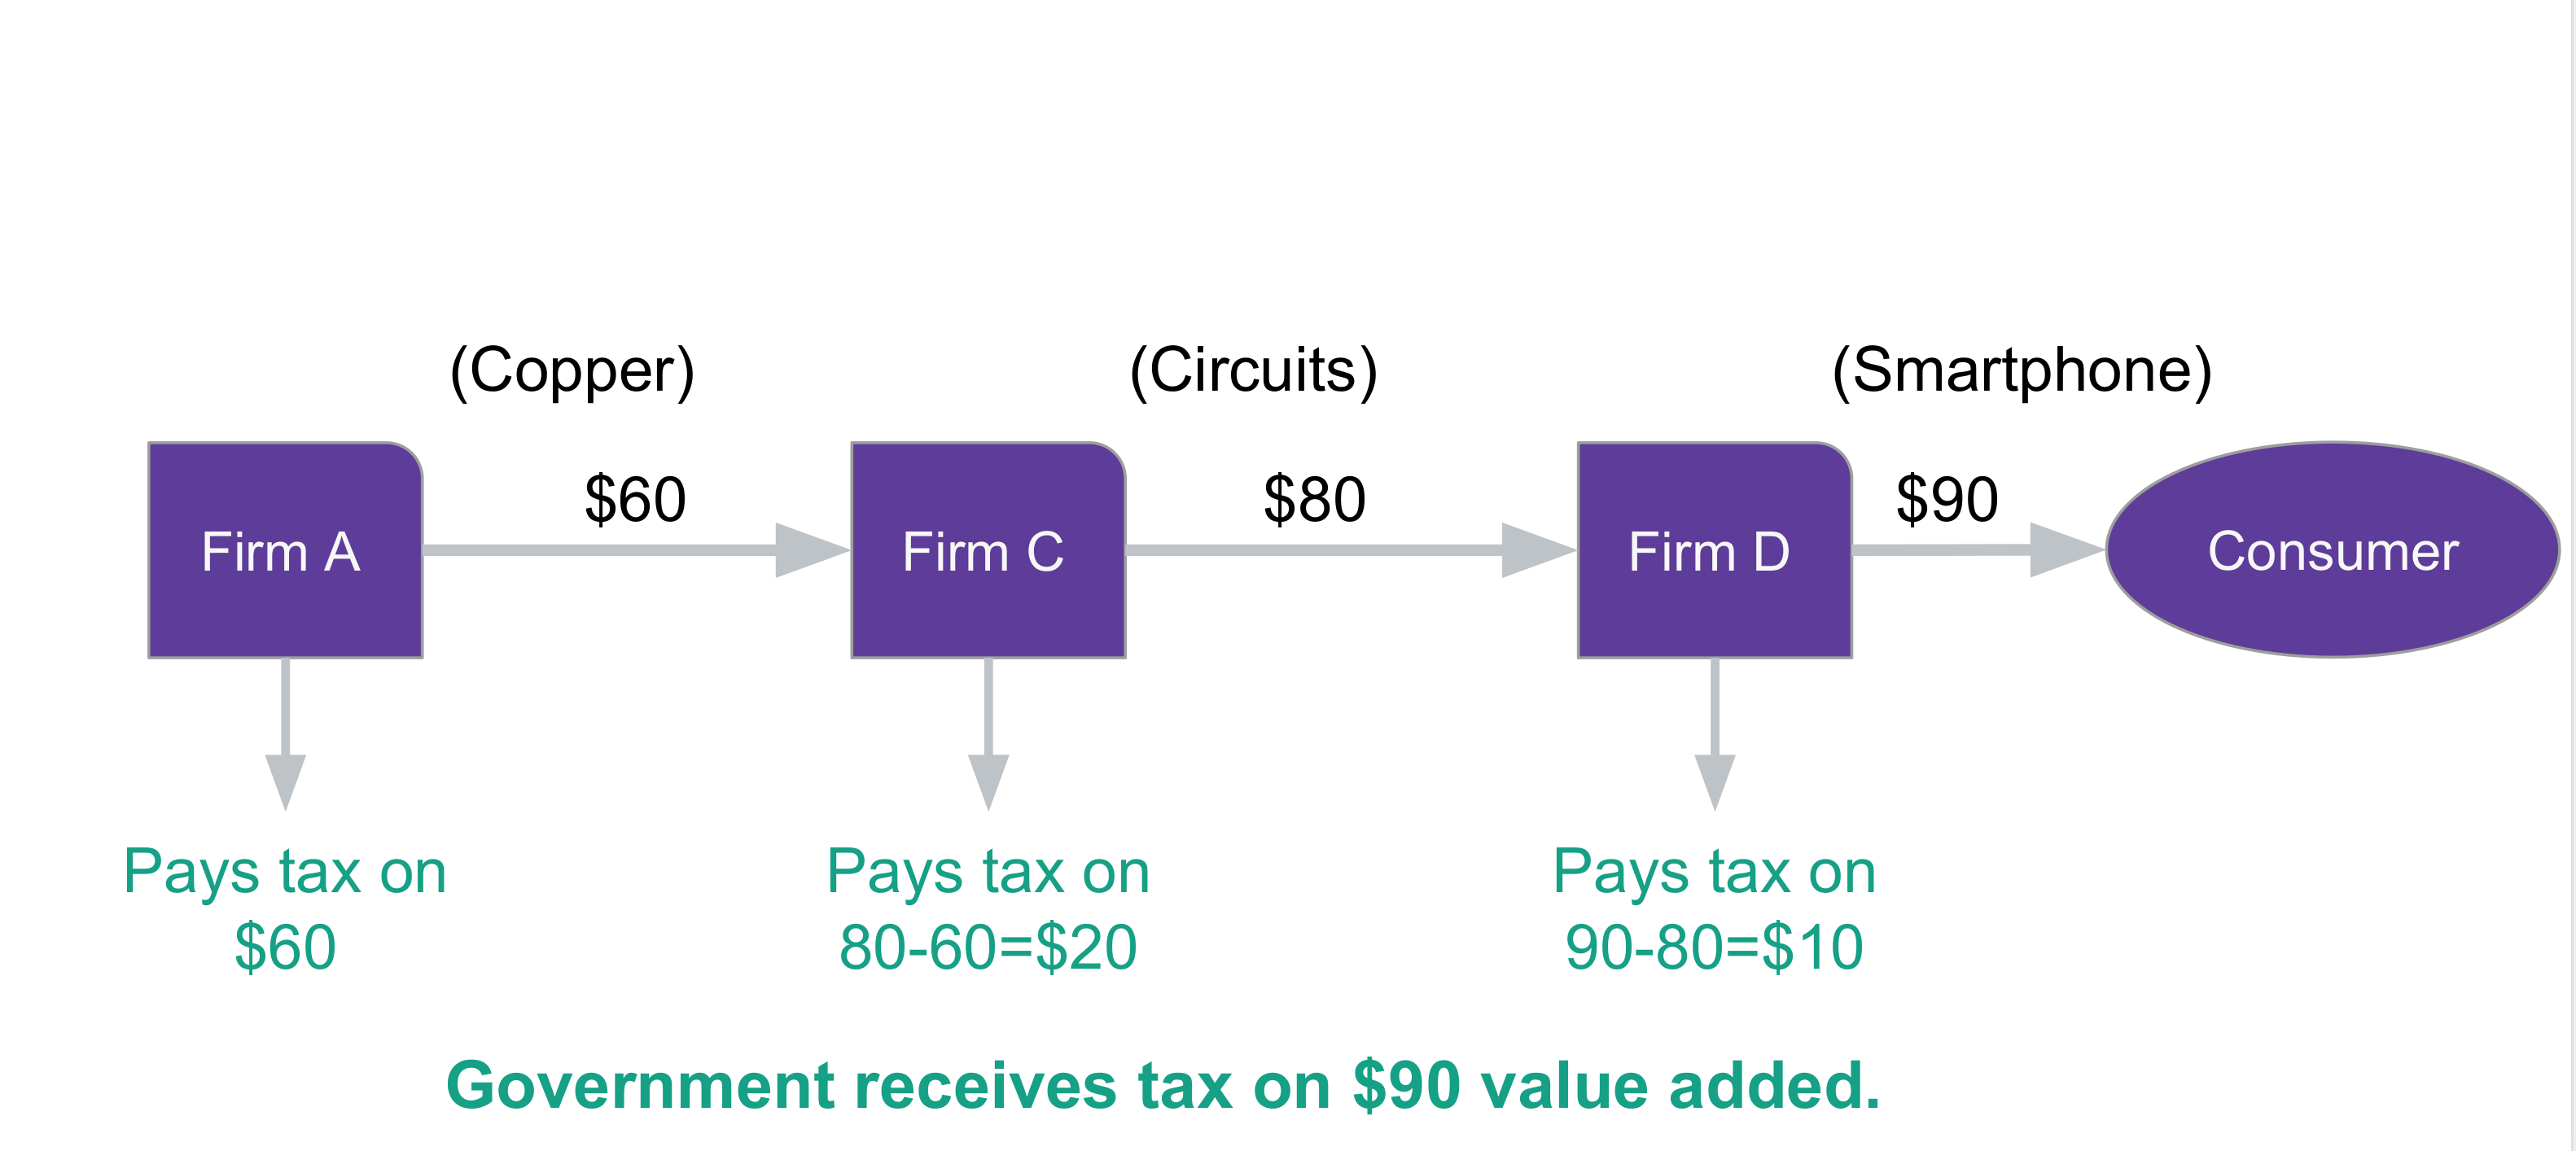
\includegraphics[width=1\textwidth]{graphs/VATExample.png}
  \caption{Stylized example illustrating a value added tax transaction chain}
  \label{fig:bogus-mechanism}
\end{figure}
However, genuine firms may want to bypass the constraints imposed by third-party verification by reporting fraudulent transactions with bogus firms. Given the attention that governments in emerging economies have begun to pay to ``ease of doing business'' norms, registering a firm is increasingly straightforward. These factors have led to the emergence of bogus firms. In \cref{sec:2-mechanism}, we explain the possible mechanism through which these bogus firms operate and lead to tax evasion.

\section{A Mechanism of Bogus Firms}
\label{sec:2-mechanism}
We now propose a mechanism that allows bogus firms to operate over multiple periods. In \cref{fig:bogus-mechanism2}, we build on the stylized example by introducing the bogus firm B. The new transactions take place only on paper (i.e. are fraudulent). The actual transfer of goods stays the same as described  in \cref{fig:bogus-mechanism}. Firm D diverts \$40 out of the \$90 business-to-customer sales that it was actually making to the final consumer to firm B and reports it as a business-to-business sale.\footnote{Firm B may make a side payment to firm D as a small kickback for violating the law by misreporting. }  Firm D can do this because it makes sales to final consumers who are not incentivized to provide reports of such transactions to the tax authority, and because this does not increase financial liability of firm D to the tax authority.  

Firm B then can sell the input credit it now has to firm A by showing a sale of an amount weakly greater than \$40 to firm A. The value add of firm A is now \$19 instead of the true value which should be \$60.\footnote{Firm A will be willing to make significant payments to firm B as this reduces firm A's tax liability.} Value added by bogus firm B is \$1, and firm C and firm D have the same value added as earlier. The final value added in the system now is \$40 less relative to a fully compliant system. The surplus (tax evaded) can potentially be divided between the offending firms, i.e. A, B (bogus), and D.

A few key observations need to be highlighted. First, firm A and firm D do not need to be in the same transaction chain. It is not necessary for the eventual chain of transactions to be circular. Firm C does not benefit from the bogus transactions and need not even know about them.\footnote{We include firm C to highlight that such transactions can co-exist around genuine transactions.} Second, bogus firm B can make sales to any firm which is in need of input credits. It does not necessarily need to make such sales to firm A which is at the beginning of the transaction chain. Third, we believe that once detected it is not complicated to verify that firm B is bogus. It is a fake firm which should not exist physically at the address submitted to the tax authority.\footnote{In subsequent field work we can test this assumption} Therefore, there is no need to rigorously analyze its business related paperwork (high effort) and a visit to the location (relatively low effort) should be sufficient. Finally, after identifying bogus firm B, the revenue can only be recovered if the authority pursues firm A and reverses the input credit that firm A has claimed. Any kind of a penalty only on firm B does not recoup the revenue loss. We now describe the design of our system.

\begin{figure}[p]
  \includegraphics[width=1\columnwidth, page=4]{graphs/StylizedExample_New2.pdf}
  \caption{An example showing how bogus firms facilitate tax evasion}
  \label{fig:bogus-mechanism2}
  \floatfoot{\footnotesize Firm A and Firm D need not necessarily be in the same chain. Bogus firms can make sales to any firm which needs input credits.}
\end{figure}

\section{System Description}
\label{sec:system-description}
\subsection{Data}
\label{subsec:2-data} 

Our dataset has almost 3 years of quarterly VAT returns from the National Capital Territory of Delhi, India from 2012-13 to 2014-15 (with personal identifying information removed). This includes consolidated returns as well as transaction level information filed by an unbalanced panel of firms, $|Firms|=315,191$, and a list of firms that were previously found to be bogus by the tax authority, $|inspected \& bogus|=538$.  Returns are filed quarterly so we should ideally have data from 12 quarters. However, for the fourth quarter of 2012-13 the transaction level records are unusable and therefore we drop that quarter from our analysis, which leaves us with data from 11 quarters. We denote these as follows. $Returns_{f,t}$ for firm $f\in Firms$ in quarter $t \in Q(f)\subseteq Q \equiv \{1,2,3,5,...12\}$, where firm $f$ operated in quarters $Q(f)$ (t=4 was dropped). Every firm is either bogus or legitimate and this doesn't change over time:$class_f \in \{bogus,legit\}$.\footnote{This is an assumption, but we have good reason to believe it from discussions with the tax authority and since there are sanctions against owners of bogus firms that are found, so owners would not use their legitimate companies for this purpose.} Some firms were inspected: $inspected_f \in \{True,False\}$ and of those inspected some were bogus and some legitimate, but this is recorded in our data only for the ones that were found to be bogus.\[ label_f =y_f= 
     \begin{cases}
       \text{bogus,} &\quad\text{if $inspected_f$ and $class_f=bogus$} \\
       \text{unlabeled,} &\quad\text{if $inspected_f$ and $class_f=legit$} \\
       \text{unlabeled,} &\quad\text{if not $inspected_f$} \\
     \end{cases}
\]

When a bogus firm is inspected at time T, it is caught and stops operating, $max(Q(f))=T$. Due to confidentiality concerns, the personally identifiable information has been removed and each firm is assigned a unique identifying number so that we can follow a firm over time as well as track its presence in other firms' returns. However, we cannot link the returns to any other publicly available information on the firms. We have detailed information on the line items in the consolidated returns, $Returns_{f,t}$, as well as line items from annexures, $Transactions_{f,t}$, where each firm reports the total purchases it made from (and sales to) each other firm at each tax rate level for that quarter. 

In addition to tax return information we also have access to basic information provided by the firm at the time of registration, $Profile_f$. Firms are mandated to keep this information updated. We observe the date of registration, the revenue ward (broad geographic location of the firm), the nature of business (e.g. manufacturer, wholesaler, retailer), its legal status (e.g. proprietorship, private limited company), the other tax schemes and acts it is subject to (e.g. central excise act) and whether it is registered for international trade (import or export).

\subsection{Features}
\label{subsec:features}
Our unit of observation is the firm-quarter level. We have an observation for each firm in each quarter in which it filed a return: firm A in quarter 1, firm A in quarter 2, firm B in quarter 1, firm B in quarter 2, etc. We ensure that none of the features use data from different time periods - they are all within the quarterly observation. We detail them in this section. In \cref{subsec:multi-period} we describe how we use the firm-quarter level observations to make predictions at the firm level.

Some of our features rely on domain expertise or anecdotes from the tax authority. For example, ``VAT/Turnover ratio'' is the ratio of tax paid to total turnover. To illustrate why this feature might be predictive, in \cref{fig:bogus-mechanism2}, if firm B reported value add of \$2 instead of \$1, it would have to pay VAT for that added dollar and will also have to reduce firm A's fake input credits by \$1. Firm B is not actually carrying out any trade, and is relying on the arbitrage between firm D and firm A to make money. This implies that it wants to minimize its declared value add or, equivalently, have a low ratio between tax paid (proportional to profit) and total turnover. 

Another example of a feature we hypothesize to be predictive is the proportion of sales a firm makes to unregistered firms - these could be small firms that are not subject to reporting or they could be final customers. An unregistered firm does not claim input credits and so cannot benefit from the services of bogus firms. We would accordingly expect bogus firms to report selling a very small share of their sales to unregistered firms, and this is borne out in our (admittedly selected) data.
Our features can be divided into 3 broad sets: $X_{f,t}=featureExtraction(Profile_f, Returns_{f,t},Transactions_{f,t})$. First is the set of profile features which come from the registration information provided by the firms. The second set of features come from the quarterly consolidated returns that each firm has to file. These include variables such as total turnover, within-state turnover, the amount of VAT that was actually paid, etc. 
Finally, the third set of features come from the annexures that firms have to file along with the consolidated returns.\footnote{Based on our interactions with various tax officials, tax administrations in general do not have the capacity to rigorously use the transaction level information that is now available to them. They mostly use it only for third-party verification purposes.} These annexures cross-reference the firm's declarations of their transactions, who it sold to, and how much that other firm reported buying back. Using these annexures, we create variables such as discrepancies in reporting between clients and suppliers, the weighted VAT/Turnover ratio of client firms, the weighted VAT/Turnover ratio of supplying firms, share of sales made to biggest client, and network features such as PageRank etc. 

We refrain from using the class labels of neighbors in the network in our features because it would compromise the estimates of performance by creating leakage between training and test set, and also because we would need a point-in-time simulation to train this, since only the class labels of firms caught before a certain time period can be used as a feature when training for that time period, otherwise we create leakage from the future to the past. 

\subsection{Class Labels}
\label{subsec:class-labels} 
In this section we describe how class labels are constructed from our data, and the problems this poses.

\subsubsection{Selective Labels - Biased Training Set}
\label{subsubsec:biased-training-set} 
The labels in our training set come from a list of firms that were targeted for inspection by the tax department, inspected, found to be bogus, and subsequently had their registration canceled. This procedure creates a biased training set as the firms targeted for inspection are not random - in fact they were chosen explicitly by the tax department as suspicious of being bogus, so are not representative of the general population (see \cref{fig:onesidedlabel}). This is the selective labels problem \cite{lakkaraju2017selective}.  We do not have a way of completely eliminating the effect of this bias on performance. However, we \textit{evaluate} our performance in a way that produces bounds which are not affected by this bias. In the future we plan to carry out inspections based on our model's predictions, which would provide an unbiased performance estimate.

\subsubsection{One-sided Labels}
\label{subsubsec:one-sided-labels} 
A more serious problem with our labels is that among the inspected firms we do not have records of which firms were found to be \textit{legitimate}, and so not canceled. This is because the tax authorities do not keep records of which firms were inspected, only which ones were found to be bogus and canceled. In our data, we are unable to distinguish the legitimate but inspected firms from those never inspected. Our labels are thus one-sided: we have firms that we know to be bogus - those canceled, and firms that we do not know for sure but are likely to be legitimate - all the rest. To further clarify the difference between selective and one-sided labels, if the tax authority randomly sampled firms for inspection, this would solve the selective labels problem but the labels might still be one-sided if they only recorded the firms found bogus.

The unlabeled firms are likely legitimate since the base rate of bogus firms in the population is not very high, though we do not know it precisely. However, they are not all legitimate as evidenced by many firms in the data being caught as bogus only after operating and facilitating tax evasion for many quarters. Therefore, we do not have a labeled training set (see \cref{fig:onesidedlabel}). This is related, though not the same, as the problem of classification with noisy labels \cite{liu2016classification, natarajan2013learning}.

We define classes for all our observations in the following way. In our outcome variable, we classify firms that were found to be bogus as 1 (``bogus'') and the rest of the firms, whether never inspected or those that were inspected, found to be legitimate and not recorded, as 0 (``probably legit''). This is an acceptable starting point as bogus firms are rare in the unlabeled set. These are two classes so it seems we can solve a standard classification problem but that is not the case. There is no out-of-sample prediction to be made on some other firms that are not already labeled by this process. We are interested in predictions on the ``probably legit'' firms, since some of them may actually be bogus and we would like to target them for inspections. We will detail our solution in \cref{subsec:cvp} and \cref{sec:evaluation}. While our classifiers would fit to predict inspected and bogus firms (selective labels), as in our training data, these are nonetheless bogus firms that they are finding. Additionally, even training on the selective set, the classifiers might learn from features not used by the tax officials and improve performance for all bogus firms.

\subsubsection{Multiple Time Periods}
\label{subsubsec:multiple-time}
For each firm, the class does not change over time - a firm does not start legitimate and become bogus, or the other way around. However, a firm is supposed to file a return every quarter. We use our classification of firms to classify all quarterly observations of that firm with the class of the firm: ``bogus'' or ``probably legit''. $y_{f,t}=y_f \in \{bogus,legit\}$.


\subsection{Classifier}
\label{subsec:classifier}

\begin{figure}
  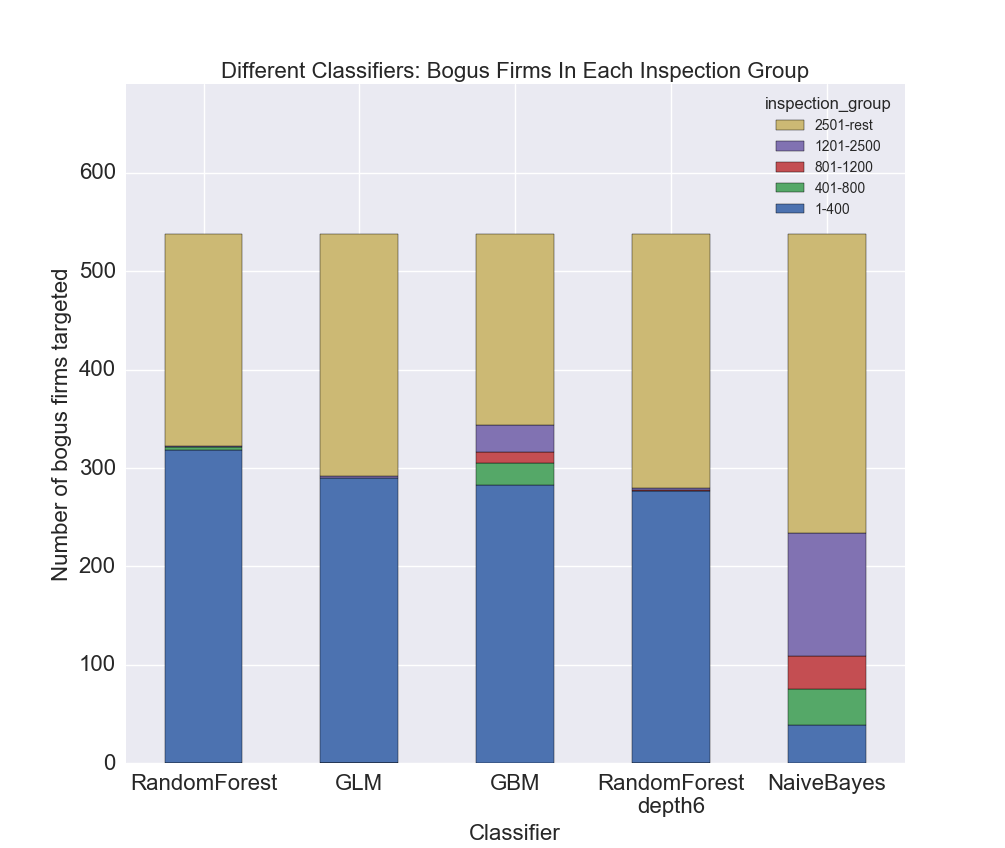
\includegraphics[width=1\textwidth]{graphs/DifferentClassifiersPerformanceByInspectionGroup.png}
  \caption{Comparison of Different Classifiers}
  \label{fig:differentclassifiers}
\end{figure}

We use a Random Forest \cite{liaw2002classification} classifier with $n\_trees=200$,\\ $stopping\_rounds=2$, and $max\_tree\_depth=20$ (the maximum depth is rarely reached in practice since the tree bifurcation stops when too few classification examples are left in a leaf) in H2O python implementation \cite{h2o_Python_module}. We selected Random Forest for its ability to handle complex dependencies between features (since not all our features are independently predictive) and combine categorical variables together with continuous variables seamlessly. 

We perform a comparison of the performance of different classifiers to see if our results are sensitive to the choice of classification algorithm. \Cref{fig:differentclassifiers} shows our results: a few  standard classification algorithms obtain similar performance. For the top 400, 800 or 1200 recommendations Random Forest performs best. The one algorithm which performs worse than others is Naive Bayes, which is unsurprising since many of the features we use are not independent and since the algorithm implementation we used also assumes Gaussian distribution for numerical features conditional on class \cite{h2o_NaiveBayes}, which does not hold with our numerical features.

\subsection{Cross-Validated Predictions}
\label{subsec:cvp}
\begin{figure}
  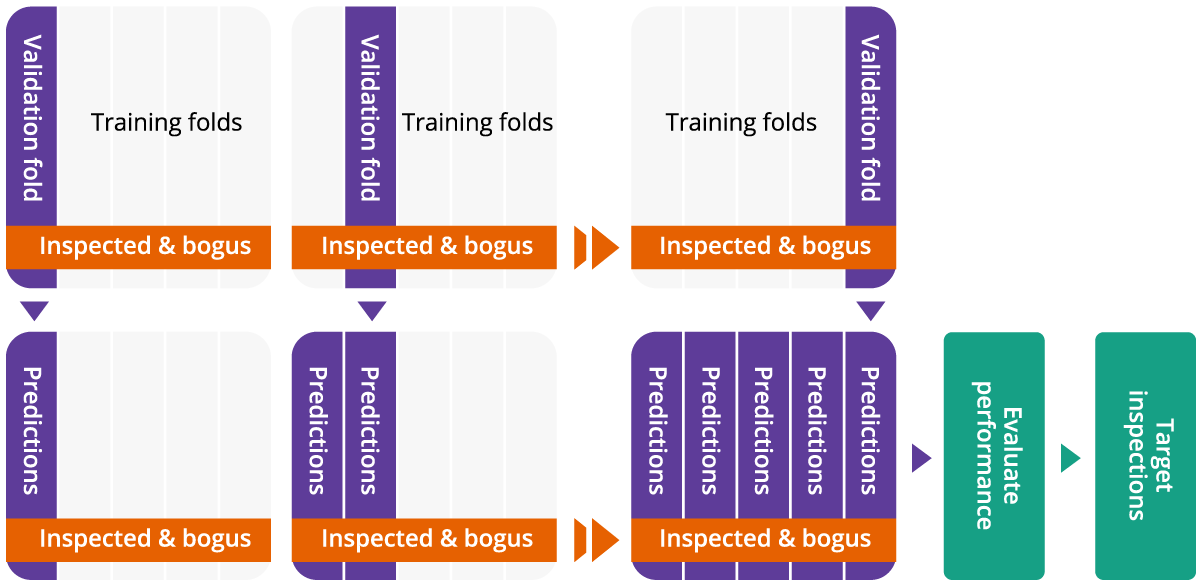
\includegraphics[width=1\columnwidth]{graphs/CrossValidatedPrediction.png}
  \caption{Cross-validated prediction procedure}
  \label{fig:crossvalidation}
\end{figure}

We have preliminarily classified all our dataset to ``bogus'' and ``probably legit'', as explained in the \cref{subsubsec:one-sided-labels}, and so it would seem that there is no more need for in-sample predictions to target inspections. However, for our real-world application, we want the model to help target inspections of existing unlabeled firms. Of the firms we classify as ``probably legit'', some are bogus and we want to find them. If we trained a classifier on all the observations (classes ``bogus'' vs. ``probably legit'') and then made predictions on the ``probably legit'' firms, we would be overfitting as a result of leakage since our model would train on certain examples and then be used to make a prediction on one of those same examples. This problem comes up in cases of prediction using noisy labels, where it is required to make predictions on the noisily-labeled data that is used for training.

To avoid this, we carry out cross-validated holdout predictions. We randomly divide our data into 8 folds. We also ensure that all quarterly observations of a firm are within the same fold, which is crucial to avoid a different type of leakage across time-periods. Formally, for each firm we draw a fold: $fold_f \in \{0,1,2,...,7\}$. We divide our data into these folds: $Fold_j = \{(X_{f,t},y_f) \space | \space f \in Firms,\space t \in Q(f), \space fold_f=j\}$. We generate predictions for all of our sample by performing 8-fold cross-validation: train on 7 folds with classes ``bogus'' vs. ``probably legit'' and make predictions on the remaining fold. We then save those holdout predictions for all of the folds - for each fold from when it was the validation fold. In this way we generate predictions for our entire dataset (see \cref{fig:crossvalidation}). To obtain predictions for firm $f$:
\begin{enumerate}
\item $\text{Train on all other folds: } Model.train(\bigcup_{j\neq fold_f} Fold_j) $
\item $\text{Make prediction: }\hat{y}_{f,t} = Model.predict(X_{f,t}) $
\end{enumerate}

To evaluate performance, we will compare those predictions $\hat{y}_{f,t}$ to the known classes $y_f$ (see \cref{sec:evaluation}). To target inspections, we plan to discard predictions for firms that are known to be bogus (since they were already canceled), and focus on the ones remaining with the highest model-predicted likelihood of being bogus. 

More than 8 folds would make for better predictions, but increase computational expense. Increasing the number of folds from 8 to 16 would increase the size of the training set from 7/8 to 15/16 - an increase of 7\% - but more than double the computation time. The extreme ideal for prediction would be leave-one-out, which would be computationally unfeasible on our dataset. Our method is not specific to the context of bogus firms, but can be used in any scenario with noisy labels and in need of in-sample prediction. 

\subsection{Multi-Period Model}
\label{subsec:multi-period}
Each firm operates and files returns every quarter, and so we have multiple observations for each firm $f$ - one for each quarter - with different feature values $\{(X_{f,t},y_f)\space | \space t \in Q(f)\}$. However, a firm is either bogus or not and this does not change with time, so predictions should be made for a firm, $\hat{y}_f$, not a firm in a specific quarter, $\hat{y}_{f,t}$. So we need to consider these different feature values but produce one prediction per firm. We do this in three steps. First, we train a single-period model on firm-quarter observations. Second, we use the single-period model to make predictions for all firm-quarter observations, $\{\hat{y}_{f,t}\}$. Third, we aggregate the firm-quarter predictions to the firm level to produce a single prediction per firm, $\hat{y}_f=Aggregate(\{\hat{y}_{f,t}\space|t \in Q(f)\})$ (see \cref{fig:aggregation}). For generality, we describe this situation as if we have full labels and separate $trainingSet$ and $testSet$, but we combine this approach with our approach for one-sided labels.

\begin{figure}
  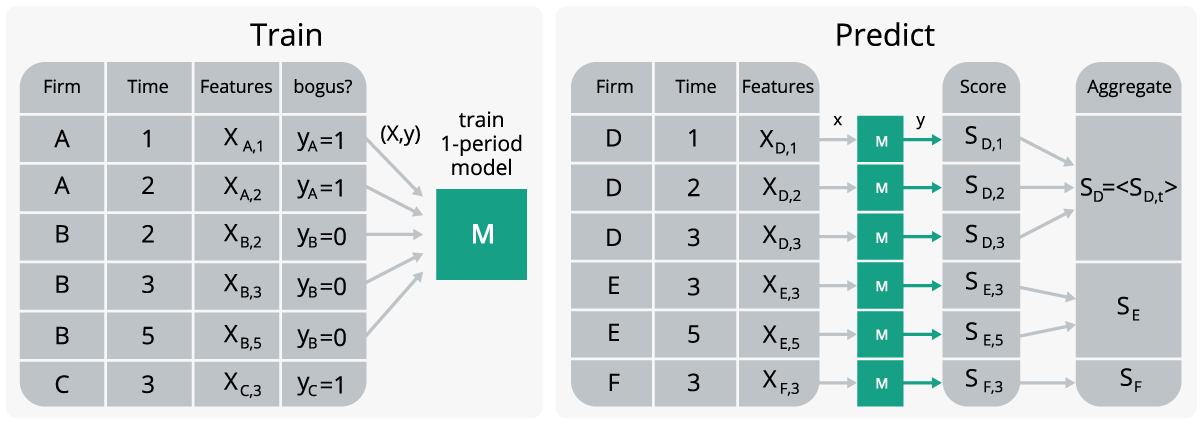
\includegraphics[width=1\columnwidth]{graphs/MultiplePeriodPrediction.png}
  \caption{Generating firm level predictions from firm-quarter level data points}
  \label{fig:aggregation}
\end{figure}

\subsubsection{Single-Period Model}
\label{subsubsec:single-period-model}
Each firm  $f$ has multiple firm-quarter data points, all classified according to the class of that firm. We use all these points to train a single-period model: \[Model.train(\{(X_{f,t},y_f) \space | \space f \in trainingSet\})\] In our case, $trainingSet$ is simply all folds other than the one to which firm $f$ belongs. Rather than taking only one observation per firm or re-weighting them so that each firm has equal total weight, this model is unaware of the fact that different observations belong to the same firm (or to different quarters) and treats them all independently (see left panel in \cref{fig:aggregation}).  This might affect performance depending on the behavior of the same firm in different quarters and how much marginal information each observation adds to the classification problem. If features in different quarters by the same firm are identical, then our procedure only introduces unbalanced duplication. If they are different, then different time-periods add valuable training examples that are all separate pieces of evidence for what bogus firms look like and our procedure is justified. Our procedure may also result in biased data based on whether firms were caught early or late, since those caught later operate in more quarters and so have more data points on which to train on and would influence the classifier more.

\subsubsection{Single-Period Predictions}
\label{subsubsec:single-period-prediction}
We use our single-period model to make predictions on firm-quarter observations: \[\hat{y}_{f,t}=Model.predict(X_{f,t})\] The model is unaware of the fact that different observations may belong to the same firm. These predictions are model-predicted probabilities of being bogus - numbers between 0 and 1, where 1 is certainty of being bogus, and 0 is certainty of being legitimate. In this way we generate predictions for all the observations, using for each firm all folds that do not contain that firm as described in \cref{subsec:cvp} (see right panel in \cref{fig:aggregation}).

\subsubsection{Aggregating Predictions to The Firm-Level}
\label{subsubsec:predictionaggregation}
Eventually, we want to make a single prediction for a firm by combining the information available across quarters. We do this by aggregating the single-period model-predicted probabilities at the firm level to create final predictions (see \cref{fig:aggregation} right panel): \[\hat{y}_f=Aggregate(\{\hat{y}_{f,t}\space|t \in Q(f)\})\]

We experimented with different functions for aggregating single-period predictions. For example, if a firm's single-period predictions were 0.1, 0.2, 0.6 then the arithmetic mean aggregating function would produce a score of $0.3$, whereas the maximum aggregating function  (maximum model-predicted probability of being bogus across periods) would produce $0.6$. In practice, the arithmetic mean works best, only slightly ahead of the maximum score function. We therefore end up using the arithmetic mean as our aggregating function. Other functions that we tried were ``take the score of the first (last) period for that firm'', and ``maximal (minimal) score for that firm across all periods''.  

There are other approaches that can potentially address the multiple time period problem. For example, aggregating the features before generating predictions instead of aggregating predictions, or treating each firm as a single observation and the list of its quarterly VAT returns as the corresponding feature vector. All approaches have their own challenges and we picked the one that we seemed least problematic. If we aggregate feature values before generating the predictions, we might end up losing the variation in  multiple observations of the same feature. If we combined all quarters to ensure that each firm had a single observation, then the same feature across time will be treated independently, so in effect we’re reducing the number of points in the training set. Moreover, entry and exit of firms in different time periods will result in the dataset having a lot of NULL values.

Our chosen approach is not specific to multiple time periods. It is applicable whenever there are several identical-format data points for each object of classification (the firm, in our case) but classification must be made at the object level. For example, different doctor visits per patient,  or fraud detection based on multiple online purchases by the same customer, or many monthly behaviors of the same object.

\section{Evaluation of Performance}
\label{sec:evaluation}
\subsection{Top Recommendations}
\label{subsec:top-recommendations}
We are constrained by the number of firms the tax authorities can physically inspect, and so we aim to provide a ranked list of suspicious firms. Performance on other parts of the distribution has no real world implications. We rank our firms in descending order of model-predicted likelihood: $rank(f1) \leq rank(f2) \text{ iff } \hat{y}_{f1}\geq \hat{y}_{f2}\text{.  } rank(f) \in \mathbb{N}$. We take a few realistic numbers of top recommendations and check our model's success on those - of these top $N$ firms predicted to be bogus by our model, how many are known to be bogus? Formally, $\text{bogus in top N}=|\{f\space|\space rank(f)\le N,y_f=bogus\}|$. 

Of our top 400 most suspicious firms, we find 75\% to be actually bogus. Of the next 400 - 12\% are actually bogus. Of the next 400 - 6\%, of the next 1300 - 3\%, and of the general population - a negligible fraction (see \cref{tab:AllTimeCVPerformance}). Our model finds more than 75\% of firms labeled ``bogus'' in the top 2,500 recommendations - less than 1\% of firms, which is very good performance. Moreover, recall that the ``probably legit'' firms in this dataset are not necessarily legitimate - they could be bogus unknown to us because they were not inspected - so these numbers for the true-bogus rate in $N$ inspections are underestimates. See \cref{fig:AllDataPerformanceTop1000} for more fine-grained results on the top 1000 recommendations.


\begin{table}
  \begin{tabular}{lrrr}
  	\toprule
	  {\small\textit{Inspection}}  & {\small\textit{Firms}}  &  {\small\textit{Total Bogus}}  &  {\small\textit{Bogus Firms}} \\
    {\small\textit{Group}} & {\small\textit{Inspected}} &{\small\textit{Firms Caught}} & {\small\textit{Caught/Inspection}}\\
    \midrule
              1 - 400 &              400 &                     305 &                           0.76 \\
            401 - 800 &              400 &                      48 &                           0.12 \\
            801 - 1200 &              400 &                      24 &                           0.06 \\
          1201 - 2500 &             1300 &                      29 &                           0.02 \\
          2501 - rest &           313229 &                     132 &                           0.00 \\
    \bottomrule
  \end{tabular}
  \caption{Model performance on top recommendations}
  \label{tab:AllTimeCVPerformance}
  \floatfoot{\footnotesize Using data from all time periods and cross-validated predictions.}
\end{table}
 
\subsection{Top Recommendations - Maximizing Revenue}
\label{subsec:top-recommendations-revenue}
From tax authority's perspective, we want to maximize expected revenue captured, and not merely the likelihood of finding a bogus firm. Small firms will only account for a small amount of tax evaded, and larger bogus firms will account for a much larger amount.\footnote{More precisely, this is determined by the amount of tax input credits claimed, the \$40 in the stylized example above.} We would therefore want a different ranking, in descending order of expected recovered revenue and not of model-predicted likelihood of being bogus. We use the following procedure to make such recommendations.

\begin{figure}
  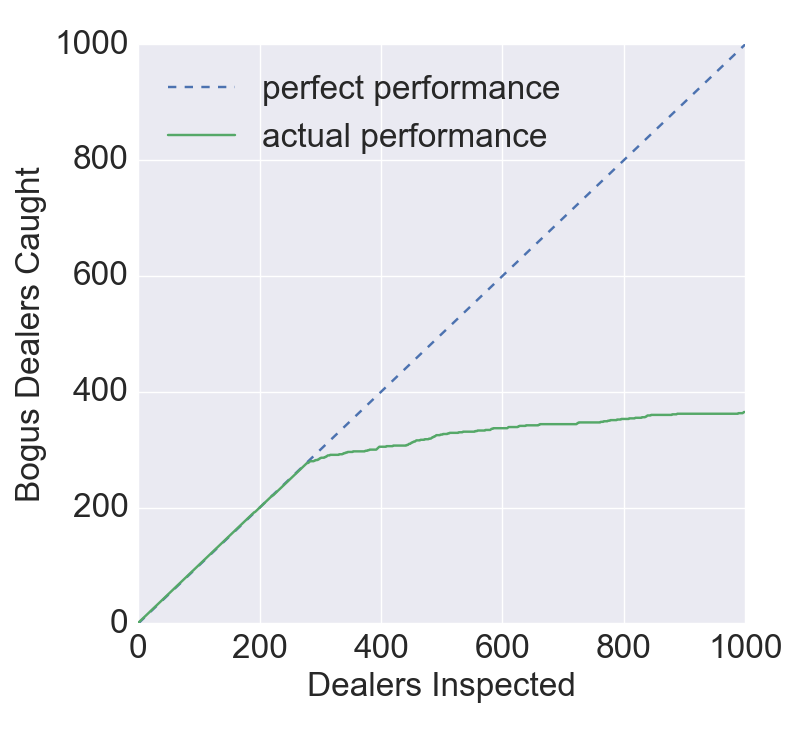
\includegraphics[width=0.5\textwidth]{graphs/PerformanceAllData_v2.png}
  \caption{Model performance on top 1000 recommendations}
  \label{fig:AllDataPerformanceTop1000}
  \floatfoot{\footnotesize Using cross-validated predictions on all time periods. The x value is the rank N of suspicious firms and the y value is the number of firms out of those N that are bogus. The dashed y=x line indicates perfect performance, i.e. every firm inspected is bogus. Model performance is near-perfect for the first 250 predictions, then starts to level off.}  
\end{figure}
First, calibrate the model, so its score is an unbiased estimate of the actual probability of being bogus: $E[y_f|\hat{y}_f\approx a]\approx a$. For example, of firms with model score of 0.1, about 1 in 10 should be bogus, for those with model score  0.01 about 1 in 100 should be bogus, etc. This is not automatically the case for predictive models (e.g. Naive Bayes, which tends to extremes with more and more dependent features). Our model turns out to be very well calibrated (results not reported).

Second, calculate expected revenue recaptured by taking the amount of input tax credits the suspicious firms claim (as depicted in \cref{fig:bogus-mechanism2}) as the lost revenue to be recaptured, and multiplying it by the calibrated model score as the probability of a firm being bogus: $ExpectedRevenue_f=\hat{y}_f\cdot InputCredits_f$. We then rank all firms in descending order of the expected revenue captured, and recommend the top ones. On our data the performance of this method in terms of revenue is comparable to the earlier described method and therefore we do not report the results.

\subsection{Different Feature Sets}
\label{subsec:feature-sets}
We have constructed 3 distinct feature sets which we use together in our model: features constructed from the individual firm's returns ($Returns_{f,t}$), features constructed from the firm's dealer profile ($Profile_f$), and features constructed from the network of firms and their trading partners ($Transactions_{f,t}$). We now disaggregate those feature sets and evaluate the performance of the model with each possible combination of feature sets. See \cref{fig:AllDataPerformanceDifferentFeatureSets} for the results. There is a three-way tie between feature sets that contain $Profile_f$ and one other feature set, so that the addition of the third one makes no discernible difference.

\begin{figure}
  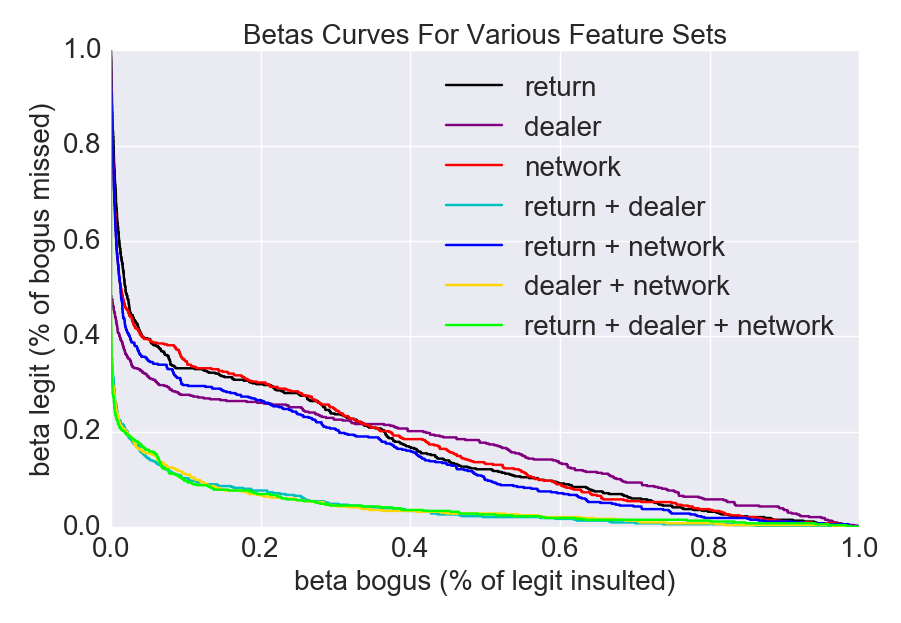
\includegraphics[width=0.4\textwidth]{graphs/PerformanceDifferentFeatureSets_v3.png}
  \caption{Betas curves for different feature sets}
  \label{fig:AllDataPerformanceDifferentFeatureSets}
  \floatfoot{\footnotesize The beta curve is 1 minus the ROC curve. As we vary the classification threshold, the x value tracks the fraction of ``probably legit'' firms that will be insulted by getting inspected ($\beta_{bogus}$); the y value tracks the fraction of bogus firms that will be missed by being classified as legit ($\beta_{legit}$). A lower curve indicates better performance.}
\end{figure}

\subsection{Point In Time Simulation}
\label{subsec:PITSimulation}
Our performance estimates so far may seem unrealistic. If we use our model in a real-world scenario, we will not have access to all returns by all firms and will not be required to predict retroactively which firms were caught as bogus and which were not. In a realistic scenario, we would have the returns of all firms up to a certain point in time, and would have to predict which of the firms still operating are likely to be bogus and need to be inspected. Some of those inspected would actually turn out to be bogus. We therefore propose another metric to gauge our performance: point-in-time simulation. 

We build a model based on the state of knowledge and data at a certain point in time T, when the returns for quarter T have been filed but inspections between quarters T and T+1 were not yet performed. We blind our model to all information in the dataset obtained after time T - we do not consider ``future'' tax returns of firms from times greater than T. For our training purposes we only use firms that had already been classified as bogus and canceled by time T. This means that bogus firms caught after time T are classified in the training set as legit. We argue that this strategy simulates the state of knowledge and data at time T (\cref{fig:PointInTimeSchematic}, a panel describing T=3).
\[SimulationTrainingSet_T = \{(X_{f,t},\tilde{y}_{f,T}) | t\le T\}\]
\[   
\tilde{y}_{f,T} =
     \begin{cases}
       \text{bogus,} &\quad\text{if $y_f=bogus$ and $max(Q(f)) \le T-1$} \\
       \text{legit,} &\quad\text{if $y_f=bogus$ and $max(Q(f)) \ge T$} \\
       \text{legit,} &\quad\text{if $y_f=legit$} \\
     \end{cases}
\]
\[SimulationTestSet_T = \{(X_{f,t},y_f) | t\le T,max(Q(f)) \ge T\}\]

\begin{figure}
  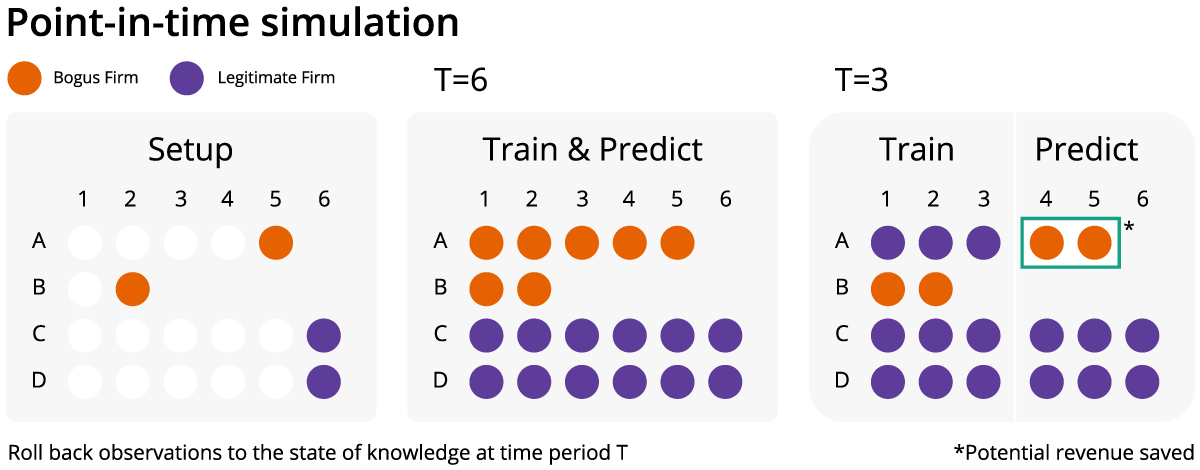
\includegraphics[width=1\columnwidth]{graphs/PointInTimeModel.png}
  \caption{Illustration of point-in-time simulation at T=3}
  \label{fig:PointInTimeSchematic}
\end{figure}

We then run our prediction algorithm on this state of the data to generate top recommendations for firms still operating at time T. We evaluate performance by using, for the validation set, the real class of firms which were later caught as bogus ($y_f=bogus$ and $max(Q(f)) \ge T$). Allotting $N$ inspections based on our simulated model's top recommendations, we determine the number of bogus firms, which were later caught by the tax authorities, that our model would have ranked in the top $N$ in time $T$. By summing the input tax credits that these recommended bogus firms claim in time periods greater than T, we can estimate how much lost revenue could have potentially been saved by using our model.

For example, suppose there are 4 firms: A, B, C, D and 6 time-periods as in \cref{fig:PointInTimeSchematic}. Firm A was inspected and identified as bogus in t=5, and firm B was inspected and identified as bogus in t=2. At T=6 after all returns have been filed and inspections have taken place, we know the class of all firms and so we know that firms A \& B are bogus. Our previous performance estimates use this state of knowledge to train, predict and evaluate performance (T=6 panel). 

Now when we simulate the state of knowledge at time T=3, we would have our features for t=1,2,3. We would also know that firm B is bogus, since it was caught and canceled after quarter t=2 and so did not file a return in quarter t=3. However, we would not know that firm A, which would be caught and canceled after quarter t=5, is bogus, and so it would be labeled as ``probably legit''. Firms C \& D would also be labeled as ``probably legit''. We now train our model on all observations from t=1, 2, 3. We use these observations to make predictions on firms A, C, D but not on firm B - since it was already canceled and is no longer operating so there is no point in targeting it for inspections. Suppose that firm A is targeted for inspection based on its features in t=1, 2, 3. We can now discern ourselves to its real class, ``bogus'' - in reality only discovered at t=5, and see that we correctly identify it as bogus in T=3. If we were to conduct inspections based on these recommendations, firm A would not have been able to operate in periods 4 and 5, and the tax evasion it facilitated in those periods would have been avoided and revenue loss averted (\cref{fig:PointInTimeSchematic}, T=3 panel, marked by asterisk). 

This assumes no substitution, i.e. that if a firm was using the services of a bogus firm to evade taxes and that bogus firm is caught and canceled, then the client firm does not find another bogus firm to facilitate its tax evasion but instead pays the required tax. We intend to rigorously test to what extent this is the case in future work using a randomized controlled trial. To adjust our revenue implications to substitution, we can multiply the revenue captured by a factor between 0 and 1 indicating what fraction of the evasion was not substituted.

Results of point-in-time simulations for various times T are detailed in \cref{tab:PointInTimeResults} and plotted in \cref{fig:PointInTimePerformanceArea}. Even based on only a few time periods, our simulated model succeeds in targeting a sizable fraction of bogus firms in the first 400 inspections (0.12\% of firms). Almost all bogus firms targeted by the model fall in the top 400 recommendations, with the other recommendations contributing very little. The performance improves when time advances from T=2 to T=4 since the model has more labels for training (labels from t in \{1,2,3\} vs. \{1\}), but then declines towards the end of the dataset when there are not many bogus firms left to be detected. Note that these simulations are not disjoint - many of the firms we would have caught in T=2 are the ones we would have caught in T=4, 6 and so on. So we cannot simply add up the numbers of firms caught and revenue captured, but have to select one. Of course, these are underestimates since some of the most suspicious ``probably legit'' firms are in fact bogus firms that were never inspected.

The number of bogus firms caught and the revenue saved are also calculated per inspection, showing an excellent hit rate of about 1 in 3 and extremely high returns for the first 400 inspections.  In all, the top 400 recommendations catch between 20\% and 40\% of all known bogus firms operating at that time.

\begin{table*}
  \begin{tabular}{rrrrrrr}
  	\toprule
	  &&& {\small \textit{Revenue Gained}}& {\small \textit{Revenue Gained}}&&{\small \textit{Revenue Lost}} \\
    & {\small \textit{Total Bogus}} &{\small \textit{Bogus Firms}}&{\small \textit{by Inspecting}}&{\small \textit{per Inspection}}&{\small \textit{Total Bogus}}&{\small \textit{from All Bogus Firms}}\\
  {\small \textit{T}}&{\small \textit{Firms Caught}}& {\small \textit{Caught/Inspection}}&{\small \textit{Entire Group (USD Millions)}}&{\small \textit{(USD 000s)}} &{\small \textit{Firms in the Sample}}&{\small \textit{(USD Millions)}} \\
    \midrule
    %&&&&&& \\
    2 &  94&0.24 &19.44&48.60&416&49.40\\
    4 & 155&0.39  &43.19&107.97&412&108.38\\
    6 & 156&0.39  &25.48&63.70&437&63.84\\
    8 & 157&0.39  & 9.38&23.46&395&26.43\\
   10 &  46&0.11  &1.70 & 4.24&114&4.52\\
   12 &  10&0.02  &      0&   0&22&0\\
    \bottomrule
  \end{tabular}
  \caption{Point-in-time simulation performance for the 1-400 inspection group}
  \label{tab:PointInTimeResults}
  \floatfoot{\footnotesize Each row shows the impact of inspecting the top 400 firms by model score: the number of known bogus firms that would have been found, and the revenue saved. The last two columns show the total number of bogus firms left to be caught at that time T, and the future revenue lost due to their activity.}
\end{table*}

\subsubsection{Revenue Implications}
\label{subsec:revenue-implications}
Point-in-time simulation also enables us to see how much additional revenue could have been gained by correctly targeting a bogus firm. We now estimate this effect by taking the top 400 firms that our point-in-time model would have recommended for inspection, and collecting the potentially gained revenue due to earlier-than-actual inspections of those of them that were later discovered to be bogus. For example if in reality a bogus firm was caught by the tax authorities after quarter 4, but our model  would have recommended it for inspection in quarter 2, then the bogus firm would have been caught and its evasion in quarters 3 \& 4 prevented - which is the revenue gained. We estimate revenue savings in the order of several tens of thousands US\$ recovered per inspection of the 1-400 inspection group in the earlier and middle time periods. In later periods, bogus firms were not yet identified by the tax authorities in our data and so mechanically the numbers are lower (see the results in \cref{tab:PointInTimeResults}). 

\begin{figure}
  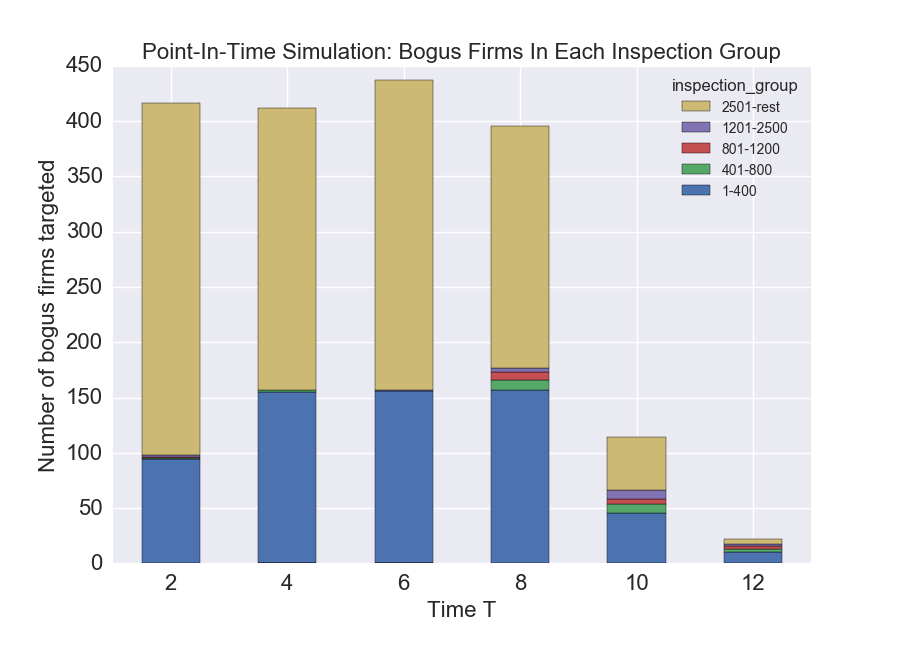
\includegraphics[width=0.4\textwidth]{graphs/PointInTimePerformanceAggregate.png}
  \caption{Point-in-time simulations performance}
  \label{fig:PointInTimePerformanceArea}
  \floatfoot{\footnotesize For a point in time simulation in time T (x axis), out of all the bogus firms still operating, the chart shows the number of bogus firms that fall in each inspection group.}
 \end{figure}


\section{Future Work and Conclusion}
\label{sec:2-conclusion}
The purpose of this paper is to assess if a machine learning tool can be effective in catching bogus firms, in reducing the effort required by tax inspectors, and in eventually increasing tax collections. By creating a model from VAT returns from the state of Delhi, India and by analyzing the performance of the model, we provide evidence that targeting inspections based on a ML model could be highly beneficial even in a low compliance high evasion setting. Our results indicate that by using our tool the tax administration can prevent fraud up to \$15-45 million. Given that such data exists in many tax jurisdictions and that anecdotal evidence suggests that such false paper trails are a common problem, our work should have high policy relevance both within India and elsewhere.

The field level efficacy of the results that we have described in this paper needs to be investigated. We need to evaluate whether our work reduces the effort required by tax inspectors, and more importantly, does it improve revenue collections. A rigorous way to assess the reduction in administrative effort due to our model would be to target future inspections by comparing the recommendations of our model with a list of recommendations prepared by a team of tax officials and then inspecting the firms recommended by each and comparing performance. We are working with the Delhi tax authority to implement this.

Simultaneously, we aim to improve the results of our model by working closely with the tax authority in Delhi to conduct tax inspections on firms recommended by our model. We intend to stratify these inspections by our model score, inspecting firms throughout the model score distribution. Stratified inspection would provide a representative training set. On the other hand, inspecting the most likely bogus firms would provide more representatives from our rare class. We are not sure how to trade off those one vs. the other, but a similar point-in-time simulation exercise with our data where we only obtain information from our targeted inspections could shed light on this question.

Finally, recovering the revenue loss which can be directly attributed to bogus firms is not trivial. Often, the owners of these bogus firms can not be found at their declared addresses. Even if caught, they themselves have not benefited from the entire tax evasion. In fact, they have been key contributors to their trading partners who have managed to reduce their declared tax liability by interacting with these bogus firms. To do the actual revenue recovery, it is important to pursue the firms which interact with the bogus firms. Moreover, it is possible that even if the transactions that the trading partners declare with bogus firms have been canceled, the trading partners substitute these transactions to other yet to be identified bogus firms. If our system is deployed and bogus firms try to adapt, we will face a scenario of adversarial machine learning. All these are important questions which we hope to study as part of our future work.

%\section{Bibliography}
%\label{sec:bibliography}

%\bibliographystyle{plainnat}
%\bibliography{bib_chapter2}
                         %

\chapter{Red Tape? The Revenue Impact of the VAT Filing Thresholds}
\section{Introduction}
\todo[inline, caption={Change Intro Para}, color=green]{The first para looks like a replica of my other paper. Need to change it.}
Tax collection has repeatedly been shown to be crucial for state development \citep{besley2014developing}. In this context, value-added tax (VAT) has been proven to be an effective tool to raise revenues \citep{keen2006vat}. The VAT systems across the world are, however, afflicted with size-dependent regulations. Such policies form an elementary part of the VAT administration across countries, with both the VAT registration thresholds and the VAT reporting frequency thresholds being dependent on the reported firm revenue.

\todo[inline, caption={Liquidity concerns}]{In the public version, we have to talk about liquidity.}
\todo[inline, caption={Optimal literature}]{What does the literature say? Anyway for us to say, econ 101 says that this should not matter}
However, the benefit of such size-dependent regulations to the tax authority is unclear. First, the tax authority may prefer to receive as much information as fast as possible. Second, the government might be liquidity constrained, so that it also prefers to receive the VAT payments from the firms at as high frequency as possible. On the other hand, the literature has provided theoretical arguments that the government should economize on administrative and compliance costs by exempting small firms from taxation \citep{dharmapala2011tax}. Such optimizing concern might be even more important for low- and middle- income countries, where compliance costs are of first order concern. Indeed,  compliance costs, relative to firm size, might be greater for smaller companies - with little benefit to the tax authority \citep{internationaltaxdialogue2007,internationaltaxdialogue2013}. In the context of many countries, firms close to the VAT registration threshold actively manipulate their reported revenues in order to avoid registering for VAT \citep{onji2009response,gebresilasse2016firm,liu2017vat,harju2016effects, boonzaaier2017small}. Furthermore, recent work has shown that firms also respond to the VAT filing or the so-called administrative thresholds \citep{asatryan2017responses}. 
\todo[inline, caption={Reframe Armenia paper}]{We have to be careful about how we talk about armenia paper. In its current form it is not clear how we are different from it.}

In this paper, we use an administrative dataset from the state of Delhi in India to first show that a policy which mandated different frequencies of filing based on reported turnover resulted in bunching of firms below the thresholds at all levels. Using the change in these reporting policies, we provide further evidence that such sharp bunching indeed occurs due to the VAT reporting frequency thresholds. Second, we calculate the VAT revenue losses due to such bunching and document the longer-term impact of the VAT reporting frequency thresholds. Finally, the subsequent withdrawal of the policy allows us to show that in a regime with size-dependent reporting requirements, more frequent reporting does not lead to greater levels of VAT collection.
\todo[inline, caption={Redo}]{The above paragraph is the replica of the abstract}

Our paper is the first, apart from \citet{asatryan2017responses}, to carefully investigate the firm responses to the VAT filing thresholds on the intensive margin. The unique setting in the state of Delhi in India allows us to simultaneously look at the firm responses at several different levels of thresholds. A careful analysis of the VAT filing thresholds fills an important gap in the literature: while the VAT registration thresholds are present in almost all countries with VAT administration, the VAT filing thresholds are also ubiquitous. 

Many countries have a uniform VAT reporting regulation on either a monthly (e.g., Argentina, India [GST]), or a bi-monthly (e.g., Barbados), or a quarterly (e.g., Cyprus) frequency. Moreover, there are many countries with policies that mandate frequency of VAT reporting based on firm size. Out of a 2015 sample of 103 countries for which we could determine with certainty, 39 countries size-dependent frequencies of VAT reporting and payments.\footnote{Based on survey of the data from \citet{ey2015worldwideguide}.} Among these there are both high-income (e.g., Austria, Germany, Denmark, Finland, France, Ireland, Spain, UK, etc.) as well as low- and middle-income (e.g., Botswana, Colombia, Mauritius, Philippines, South Africa, Swaziland) countries. If firms misreport their revenue in order to avoid filing (and remitting) VAT returns more frequently, it is important to understand the associated costs to the VAT collections. 
% * <shekhar.mittal@gmail.com> 2018-05-08T04:09:10.274Z:
% 
% Need to rephrase the above line.
% Why would a fiscally constrained government care? How does a greater frequency benefit that government?
% ^.
%Therefore, it is crucial to understand how firms respond to such size-dependent regulation more generally, and specifically to the VAT filing thresholds.

Before answering this question empirically, it is important to understand what is the optimal ``first-best'' policy with regards to VAT filing frequencies. A liquidity constrained government, which might be the case in  low- and middle-income countries, may prefer to receive the VAT reports and the associated payments with as high a frequency as possible. On the other hand, very high frequencies of VAT reporting and payments may  impose a significant burden on firms, especially on smaller ones. The trade-off is relatively clear: while the government prefers, for several reasons, to obtain information and the VAT payments as frequently as possible, it effectively subsidizes smaller firms - those, eligible for VAT - by imposing less stringent filing requirements on them. The problem occurs when such policies result in the firms actively avoiding filing more frequently, by either underreporting their actual revenues, or by under-producing and thus intentionally reducing their growth. Both of those channels are problematic: The first one creates an environment which via the choice of policies fosters a culture of evasion and avoidance, which is especially troublesome for the low- and middle-income countries. The second, underproduction channel, results in production inefficiencies, keeping the economy below its potential. In the paper, we provide a simple welfare analysis, by calculating the minimum compliance costs needed at the level of each of the reporting categories (annual, bi-annual, quarterly, and monthly) for the policy to be optimal, despite the revenue costs incurred by the tax authority. 
\todo[inline, caption={State the reasons}]{What are the reasons alluded to above?}
\todo[inline, caption={SM: Reason for relief to smaller firms}]{Empirically find out how much revenue is coming from the top firms.}


\todo[inline, caption={Policy of interest and results}]{New para: We have to describe the policy and the results}
The paper is organized as follows. The following section describes some of the related literature. \Cref{sec:background} describes the VAT system in Delhi, and describes the reforms in the VAT filing system. \Cref{sec:3-data} describes the administrative level data from Delhi that we use for our analysis. \Cref{sec:methodology} explains the methodology we use for the analysis. \Cref{sec:3-results} presents the results of our analysis of the firm response, of the revenue implications, and of welfare. \Cref{sec:3-conclusion} concludes.

\section{Related Literature
\label{sec:related-literature}}

We contribute to several strands of literature. Most generally, we build on the literature on the effects of size-dependent policies on firm behavior. The literature has shown extensively that such size-based regulations can and does lead to distortions \citep{gollin1995taxes,guner2008macroeconomic}. \citet{garicano2016firm} look at the context of labor laws in France, which start to bind firms with 50 or more employees. They find, using the administrative-level firm data, that the cost of such regulations is equivalent to a 2.3\% tax on labor, and that such regulations equal to welfare costs to the tune of 3.4\% of GDP. They also show that such size-dependent regulations are effectively subsidizing small firms, at the cost to workers and to some extent large firms. In the context of taxation, \citet{almunia2018under}, show that the threshold relevant for the large tax payers unit, which monitors large firms in Spain, results in strategic bunching of the firms in order to avoid stricter monitoring by the tax authority. Finally, they show that extending stricter monitoring to small businesses would generally generate substantial welfare gains.

Such size dependent policies are ubiquitous across countries. In their cross-country study, \citet{bachas2017size} for instance find that firm size has large effects on tax enforcement and the resulting tax compliance, with negative effects on giving bribes. Importantly for our work, they show that such a size gradient in tax enforcement is the strongest in developing countries. In the VAT context, \citet{mittal2017vat} show that strengthened paper trail leads to an increase in tax collection, primarily driven by the behavior of the largest firms. 

More specifically, we add on to the wide literature discussing the VAT policy, both theoretically and empirically. \citet{keen2006vat}, for instance, discuss the problematic aspects of the VAT policy in the EU countries, particularly when specific policy aspects result in a greater propensity for tax evasion and fraud. They also look at the possibility of a federal VAT system in the US. In their book, \citet{bird2007vat} discuss the application of VAT in lower income countries, and note the particularities pertaining to developing and transition countries. According to them, many problems occur when implementing VAT in most developing and transition countries, including flawed design such as inappropriate thresholds, as well as failures in implementation such as poor administrative procedures and insufficient audit.   

Additionally, we contribute to the literature on calculating the hassle costs affiliated with filing taxes. In this realm, \citet{benzarti2017taxing} estimates the cost of filing income taxes using US income tax return data. He finds that such hassle costs are increasing with income of households. 

We also add on to the literature on the specific literature analyzing the so-called VAT registration thresholds:
in those cases, firms below a certain size are exempt from registering for the VAT system and thus from paying 
VAT. In their theoretical work, \citet{keen2004optimal} look at the optimal registration threshold in the case of VAT, and show that such a threshold will necessarily lead to production inefficiencies via the bunching below the thresholds. 

A growing literature has empirically analyzed the effect of the VAT registration threshold. The first paper to recognize the reaction of firms to the VAT registration threshold was \citet{onji2009response}, which documents that large firms masquerade as many small firms in response to the VAT registration threshold in Japan. \citet{liu2017vat} theoretically and empirically consider the VAT registration notches and voluntary registration below the VAT registration threshold in the context of the UK. Their bunching estimates, based on separate annual observations of British firms between 2004 and 2010, are in the range between 0.815 and 1.286. They furthermore look at the determinants of voluntary registrations and of the bunching behavior, listing the low cost of inputs relative to sales, high proportion of business-to-customers sales, and high product market competition as determinants of higher bunching. \citet{harju2016effects} look at the impact of the VAT registration threshold on the behavior of small Finnish firms. They find that the firms actively avoid VAT liability, and that such avoidance is directly caused by the compliance costs of VAT. Furthermore, they find that the bunching behavior persists over the long-term, implying that the VAT registration threshold permanently hinders the growth of small firms. They find a strong bunching response to the VAT notch, of 3.63. 

In the context of a developing country, \citet{boonzaaier2017small} use tax register data from South Africa to look at the effects of several discontinuities in the tax schedule on the behavior of small firms. Among other discontinuities, their work also looks at the VAT registration notch, where they find a moderate level of the bunching response, of 1. Along similar lines as the Finnish study, the work on South Africa finds that the bunching firms are less likely to show strong growth dynamics and are more like to be 'stuck' in terms of their profits and sales. Similarly, \citet{gebresilasse2016firm} look at the firm response to VAT registration threshold in Ethiopia, and estimate substantial bunching, with the bunching response equaling 4.8.  

The closest paper to ours, by \citet{asatryan2017responses}, looks at the effects of both the VAT registration threshold and the so-called administrative thresholds, on the reported revenues by Armenian firms. Their analysis shows a moderate response to the VAT filing frequency threshold, which - however - corresponds to some other regulatory thresholds. For their full sample, they find the bunching response of 1.569. Their hetorogeneity analysis shows that the response is driven up by growing firms, and by firms in the primary sector and services. Furthermore, they show, using audited tax returns, that the response is mainly driven by evasion, rather than by underproduction. Finally, \citet{asatryan2017responses} find no response to the VAT registration threshold notch. 



\section{Background}
\label{sec:background}

\section{Data}
\label{sec:3-data}



\section{Methodology}
\label{sec:methodology}
This section describes the methodology we use to derive the distributional
and other results discussed in the following section. We respectively
describe the methodology used to derive the bunching estimates, and
the methodology to identify the VAT revenue losses to the tax authority
due to the imposed reporting thresholds and the resulting bunching.
We then describe the methodology we use to show that there are no
apparent revenue benefits to the tax authority by the firms providing
more frequent information in the form of the VAT reports. Lastly,
we outline our methodology for the general social welfare analysis
of the VAT reporting thresholds.

\subsection{Bunching at Thresholds}
\label{subsec:methodology-bunching}

Throughout our bunching analysis, we focus on the local effects in
the immediate vicinity of each of the thresholds. We thus divide the
firms into bins of 30,000 Indian rupees around the low (annual firm
revenue of 1 million rupees \textasciitilde{} \$20,000) and the middle
thresholds (annual revenue of 5 million rupees \textasciitilde{} \$100,000).
Similarly, we divide the firms into bins of 300,000 Indian rupees
around the high threshold (annual firm revenue of 50 million rupees
\textasciitilde{} \$1,000,000). Once

The lower excluded area, starting at $R_{1}$ to the left of a given
threshold and ending at the threshold $T$, features a discontinuous
increase in the distributions of firms right before the threshold.
The upper excluded area, starting at the threshold $T$ and ending
at $R_{2}$ to the right of a given threshold, features a missing
mass in the number of firms immediately after the threshold. For each
threshold, we visually observe the discontinous increase in the number
of firms before the threshold and use this visual observation to find
the value of $R_{1}$. We use the convergence method, as discussed
by \citet{kleven2013using}, to find the values of $R_{2}$ for each
of the thresholds. Namely, we choose the value of $R_{2}$ so that
the area above the counterfactual distribution between $R_{1}$ and
$T$, and the area below the counterfactual distribution between $T$
and $R_{2}$ are approximately equal.

As a proxy estimate of the counterfactual distribution, we draw a
fitted fourth-degree polynomial across all observations, excluding
the lower and upper excluded area, to the left and to the right of
a given threshold. We run the following regression to estimate the
smooth polynomial: 
\begin{equation}
C_{j}=\sum_{i=1}^{4}\beta_{i}(B_{j})^{i}+\varepsilon_{j},\forall B_{j}\leq R_{1}\&B_{j}\geq R_{2},
\end{equation}
where $C_{j}$ denotes a count of firms in a given bin $B_{j}$, $T$
denotes the threshold, and $R_{1}$ and $R_{2}$ denote the beginning
of the lower excluded area range (before the threshold) and the end
of the upper excluded area range (after the threshold). Once we obtain
the estimates from (2), we then use the predicted counterfactual in
the excluded range as well, and predict the counterfactual number
of firms as follows:

\[
\hat{C}_{j}=\sum_{i=1}^{4}\beta_{i}(B_{j})^{i}
\]
We use the estimated counterfactual to estimate the bunching in the
so-called lower excluded area (to the left of the threshold), as follows:

\begin{equation}
b=\frac{\sum_{i\epsilon S}(C_{i}-\hat{C}_{i})}{\hat{C}_{lowerexcluded}},
\end{equation}
where $S$ denotes the set of values $i$, for which the bins $B_{i}$
are in the lower excluded area, namely: $S=\{i\epsilon\mathbb{N}|B_{i}\epsilon[T-R_{1},T]$.
The bunching estimate is thus the estimate of the excess mass in the
distribution of firms before the threshold relative to the counterfactual
distribution of firms, as a share of the counterfactual distribution
of firms in the lower excluded area. In particular the latter value,
$\hat{C}_{lowerexcluded}$, is calculated as a weighted average of
the counterfactual in the lower excluded area, weighted by the distance
of the actual count of firms from the counterfactual distribution,
as follows: 
\[
\hat{C}_{lowerexcluded}=\sum_{i\epsilon S}\mu_{i}\hat{C_{i},}
\]
where $\mu_{i}$is the weight of each bin $i$, constructed as follows:
\[
\mu_{i}=\frac{C_{i}-\hat{C}_{i}}{\sum_{i\epsilon S}(C_{i}-\hat{C}_{i})}
\]
We represent the counterfactual distribution of firms with a smooth
red line in all of the figures showing bunching, while we show the
values of $R_{1}$ and $R_{2}$ using the vertical red dotted lines.

\subsection{VAT Revenue Loss to the Tax Authority}
\label{subsec:methodology-revenue-loss}
To calculate the revenue implications of bunching, we assume that
the firms in the lower excluded area (with an excess mass of firms),
and the firms in the upper excluded area (with a missing mass of firms)
are directly comparable in terms of their unobservable characteristics
- apart from their reported revenue and the VAT they remit. We then
determine the revenue implication of the threshold regulation as follows.
First, we calculate the difference in the average VAT remitted by
firms in the upper excluded area and the VAT remitted by firms in
the lower excluded area. We then multiply the difference in the average
VAT remitted per firm with the extra bunching density, $B=\sum_{i\epsilon S}(C_{i}-\hat{C}_{i})$.
The revenue implications, $R$, are thus calculated as follows:

\begin{equation}
R=(VAT_{above}^{mean}-VAT_{below}^{mean})*B
\end{equation}


\subsection{No Benefits to More Information}
\label{subsec:methodology-more-information}
The key question related to the VAT reporting thresholds is why might
the tax authority in principle be interested in getting VAT reports
from firms on a more frequent basis. We test whether the tax authority
might have benefits to the firms providing more frequent (and thus
more) information in the form of more VAT collected when the firms
provide more frequent information. We proceed as follows: First, we
group all data together, so that we have a pool of observations covering
2010-2015. We then normalize the VAT collected relative to the size
of the firm in terms of its revenues. We then run the following regression
for firm $i$ in year $j$:

\begin{equation}
(VAT/Revenue)_{i,j}=\alpha+\beta\cdot NumberReports_{i,j}+\phi_{j}+\phi_{i}+\epsilon_{i,j},
\end{equation}
where $VAT/Revenue$ is the ratio of a firm- and year-specific VAT
remitted as a share of the reported firm revenue, $\alpha$ is a constant,
$NumberReports$ is the annual number of reports filed by the firm
given its reported firm size, $\phi_{i}$ and $\phi_{j}$ are the
firm and the year fixed effects, respectively (if included in the
regression specification, as shown in Table \ref{tab:Number reports regressions}),
and $\epsilon$ are the heterogeneity robust standard errors.

We additionally test the responsiveness of the VAT collected as a
share of revenue to the annual number of submitted reports by regressing
the $VAT/Revenue$ ratio on each of the reporting categories, while
having the annual reporting as the omitted category. The regression
specification for a firm $i$ in year $j$ is then:

\begin{equation}
(VAT/Revenue)_{i,j}=\alpha+\sum_{c=semiannul}^{monthly}\beta_{c}\cdot c+\phi_{j}+\phi_{i}+\epsilon_{i,j},
\end{equation}
where $VAT/Revenue$ is the ratio of a firm- and year-specific VAT
remitted as a share of the reported firm revenue, $\alpha$ is a constant,
$c$ can take three values: $semiannual$ is a dummy variable equal
to 1 if the firm filed the VAT reports at a semiannual level in a
given year, $quarterly$ is a dummy variable equal to 1 if the firm
filed the VAT reports at a quarterly level in a given year, $monthly$
is a dummy variable equal to 1 if the firm filed the VAT reports at
a monthly level in a given year, $\phi_{i}$ and $\phi_{j}$ are the
firm and the year fixed effects, respectively (if included in the
regression specification, as shown in Table \ref{tab:Filing category regressions},
and $\epsilon$ are the heterogeneity robust standard errors.

Using these regression specifications, we then estimate the relationship
between the number of annually filed reports (or the given reporting
categories) and the amount of VAT remitted (relative to the firms'
reported revenue) using simple OLS regressions.

\subsection{Social Welfare Analysis}
\label{subsec:methodology-welfare-analysis}
We conduct a very simple case of social welfare analysis. In particular, we recognize that - while not considering the potential compliance spillovers - the overall welfare in our context depends on the sum of the tax authority's, and the compliance cost incurred by the firms in our sample. Therefore, we recognize that we can calculate the minimum implicit compliance subsidy needed to be given by the tax authority to the firms in a given reporting category in order to equalize the welfare losses stemming from the bunching behavior by the firms.

We thus calculate the implicit subsidies at each threshold $i$ in the following manner, using the values of revenue losses, $R$, calculated as explained in the subsection \ref{subsec:methodology-revenue-loss}:

\begin{equation}
ImplicitSubs_i = R_i / n_j,
\end{equation}
where $n_j$ is the number of firms in the reporting category $j$ below a given threshold $i$. This implies that for the lowe threshold, we divide the revenue losses stemming from the threshold by the number of firms reporting and paying VAT at an annual level. For the middle threshold, we divide the revenue losses stemming from the threshold by the number of firms reporting and paying VAT at a bi-annual level. Likewise, for the high threshold, we divide the revenue losses stemming from the threshold by the number of firms reporting and paying VAT at a quarterly level. 

We then evaluate whether the implicit subsidies needed to equalize the revenue losses are lower than the likely compliance costs incurred by firms reporting and paying VAT at a certain level of frequency.

\section{Results}
\label{sec:3-results}
This section describes the results obtained using the respective methodologies
as discussed in the previous section. We first discuss the results
of estimating the excess bunching at the relevant VAT filing thresholds.
The second subsection discusses the calculation of the VAT revenue
loss to the tax authority due to the existence of the arbitrary VAT
filing thresholds. The third subsection shows that there are no apparent
revenue benefits of more frequent information provision by the firms.
The fourth subsection concludes by providing the relevant welfare
analysis of the size-dependent VAT filing policy.

\subsection{Bunching at Thresholds}
\label{subsec:bunching}
This section discusses the results of estimating the excess bunching
at each of the VAT filing thresholds according to the methodology
described in the subsection \ref{subsec:methodology-bunching}.

The low threshold, set at the revenue size of 1 million Indian rupees,
was relevant for the size-dependent VAT filing policy in years 1 and
2 (2010/11 and 2011/12) and mandated the change of filing frequency
from an annual to a bi-annual level. That is, instead of filing the
relevant VAT reports to the tax authority once a year, firms with
the reported revenue size above 1 million Indian rupees were required
to file their reports twice a year. As Panels A and B in Figure \ref{fig:LowestThreshold}
show, such policy resulted in the excess bunching at the threshold,
with the bunching estimates of 0.5 for year 1, and 0.28, respectively.
In years 3, 4, and 5 (2012/13, 2013/14, and 2014/15, respectively),
the threshold policy was no longer relevant, as all of the firms around
the threshold were required to file their VAT reports on a quarterly
basis. As Panels C, D, and E in Figure \ref{fig:LowestThreshold}
illustrate, there was - in contrast to years 1 and 2 - indeed no excess
bunching around the low threshold in the later years.

The middle threshold, set at the revenue size of 5 million Indian
rupees, mandated the change of filing frequency from a bi-annual level
to a quarterly level in years 1 and 2 (2010/11 and 2011/12). As such,
instead of filing the relevant VAT reports to the tax authority twice
a year, firms with the reported revenue size above 5 million Indian
rupees were required to file their reports four times a year. Panels
A and B in Figure \ref{fig:MiddleThreshold} show that such a size-dependent
policy resulted in a significant bunching, with bunching estimates
equaling 0.34 and 0.43, for years 1 and 2, respectively. Panels C,
D, and E in Figure \ref{fig:MiddleThreshold} further show that such
bunching disappears, with a much smoother distribution of reported
firm revenues, once the threshold policy was done away with in years
3, 4, and 5.

The highest threshold, set at the revenue size of 50 million Indian
rupees, mandated the change of filing frequency from a quarterly level
to a monthly level in years 1, 2, and 3 (2010/11-2012/13). In these
years, the firms above the reported revenue threshold had to file
the VAT reports to the tax authorities twelve times a year rather
than four times a year like the firms just below the threshold. Panels
A, B, and C in Figure \ref{fig:HighestThreshold} again indicate substantial
bunching due to such filing threshold, with bunching estimates equaling
2.6, 2.98, and 1.87, in years 1, 2, and 3, respectively. Panels D
and E in Figure \ref{fig:HighestThreshold} - similarly as for the
low and the middle threshold - again provide an indication that such
bunching occurs due to the threshold policy: once the threshold policy
was done away with in years 4 and 5 - with all of the firms filing
the VAT reports on a quarterly basis - the distribution of reported
revenues becomes much smoother, with no bunching at the relevant threshold
of 50 million Indian rupees.

Within each of the thresholds, we see that the bunching occurs at
roughly the same level of magnitude. For the low threshold, we see
a decrease of bunching in the second year; for the middle threshold,
we see a slight increase in the second year bunching; for the high
threshold, we see an increase in bunching from year 1 and 2, to be
followed in a decrease in bunching in year 3. Assuming that the level
of bunching is a proxy for actual compliance costs incurred by firms,
Figure \ref{fig:ComplianceCosts} uses these bunching estimates to
track the revealed distribution of compliance costs across different
revenue sizes and plots the bunching estimates on the y-axis versus
the revenue sizes for the relevant thresholds on the x-axis. While
compliance costs seem to remain more or less at the same level across
the lower two thresholds, we see a sharp increase in the apparent
compliance costs at the highest threshold compared to the lower two
thresholds. This implies that compliance costs of a differential VAT
reporting policy are generally increasing with the reported revenue
size.

\subsection{VAT Revenue Loss to the Tax Authority}
\label{subsec:3-results-revenue-loss}
This section discusses the calculation of the VAT revenue loss to
the tax authority due to the differential, size-dependent filing policy
according to the methodology described in the subsection \cref{subsec:methodology-revenue-loss}.

We thus compare the firms in the bunching region below and above the
threshold according to their VAT contributions. Table \ref{tab:VAT revenue lost}
shows that the revenue losses are substantial. For the low threshold,
the losses amount to nearly 900,000 rupees in year 1, and to nearly
500,000 rupees in year 2. These amounts are, respectively, 2.3\% and
1.8\% of the bunchers' total VAT contributions, therefore presenting
a significant loss of VAT revenues to the tax authority. For the middle
threshold, the losses are generally less substantial, amounting to
above 700,000 rupees in year 1, and above 100,000 rupees in year 2.
These amounts respectively equal 1.8\% and 0.03\% of the bunchers'
total VAT contributions in the respective years. As shown in the table,
the losses are most substantial for the high threshold, amounting
to nearly 40,000,000 rupees in year 1, and above 20,000,000 rupees
in years 2 and 3. These amounts are also the highest as a share of
the bunchers' total VAT contributions, amounting to 8.3\%, 5.2\%,
and 4.2\% in years 1, 2, and 3, respectively.

Not surprisingly, these estimates confirm the findings in subsection
\ref{sec:bunching}: bunching is not only the highest, but also the
costliest for the high threshold.

\subsection{No Benefits to More Information}
\label{subsec:3-results-more-information}
This section discusses the regressions looking at the relationship between the VAT/revenue ratio and the frequency of VAT reporting, as discussed in the methodology \cref{subsec:methodology-more-information}.

Table \ref{tab:Number reports regressions} shows the regression results
looking at the relationship between the VAT/revenue ratios and the
yearly number of VAT reports. As shown in columns 1 and 2, the relationship
is strikingly negative without including firm fixed effects in the
regression specification, implying that the greater the number of
VAT reports per year, the smaller the VAT/revenue ratio. When including
firm fixed effects in the regression specification, as shown by columns
3 and 4, the relationship turns positive but strongly insignificant.

Table \ref{tab:Filing category regressions} similarly shows the regression
results looking at the relationship between the VAT/revenue ratios
and different reporting categories, with annual reporting being the
omitted category. As columns 1 and 2 show, when not including firm
fixed effects, all reporting categories are negatively related to
the VAT/revenue ratios compared to those firm-year observations with
annual reporting. Once including firm fixed effects in the regression,
the estimates turn positive, but again remain strongly insignificant.

Our interpretation of the results of both of the sets of regressions
is that a greater annual frequency of VAT reporting apparently does
not lead to more VAT being collected, as measured by the VAT/revenue
ratios.

\subsection{Social Welfare Analysis}
\label{subsec:3-results-social-welfare}

This section discusses the ad hoc social welfare analysis conducted according to the methodology outlined in the subsection \cref{subsec:methodology-welfare-analysis}. 

Table \ref{tab:Implicit subsidies} presents the calculated implicit subsidies. The implicit subsidies from the thresholds needed to equalize welfare are very low. The implication of the result at the low threshold for year 1 - an implicit welfare equalizing per firm subsidy of 40.77 rupees (less than \$1) - implies that for the welfare change, once accounting for both the revenue losses because of the threshold and the implicit subsidies, would be negative only in the case that compliance costs borne by a given firm reporting and paying VAT at an annual level would be less than \$1, which is extremely unlikely. The implicit welfare equalizing per firm subsidy for year 2, at the low threshold is even smaller. Similarly, the implicit welfare equalizing subsidies for the middle threshold are comparably low. 

The implicit welfare equalizing subsidies for the high threshold are an order of magnitude higher, ranging from 1327.97 rupees (about \$25) in year 3 to 2990.02 rupees (about \$60) in year 1. The implication of these implicit welfare equalizing per firm subsidies is, however, similar as for the low and the middle thresholds. The actual compliance - that is, filing and paying - costs difference (quarterly level of reporting relative to monthly reporting) associated with VAT of these firms, reporting at a quarterly level is certainly higher than \$60. That means that the tax authority subsidizes these firms at a rate higher than needed for the overall social welfare impact of the thresholds to be negative. 

This analysis leads us to conclude that, while the tax authority incurs relatively large losses due to thresholds, its implicit subsidies to small and medium-sized firms are large enough to overcome the welfare losses.

\section{Conclusion}
\label{sec:3-conclusion}
In this paper, we identify bunching behavior by firms below the VAT filing thresholds, using an administrative-level dataset from the state of Delhi in India. Our unique dataset enables us to show that the bunching behavior occurs at different levels of the VAT filing thresholds, whereas the bunching completely disappears when the thresholds are done away with. The bunching is the highest for the largest firms, which indicates that compliance costs are the highest for those firms. We further document that the VAT revenue losses due to the bunching response by firms are substantial, amounting up to 8.3\% of the bunchers' total VAT contributions in certain years. The paper also shows that apparently there are no benefits to the tax authority from receiving more frequent information in terms of the VAT filing reports. Our social welfare analysis finally shows that given that the costs of compliance by the firms are likely relatively large, the net-of-implicit-subsidies welfare impact of the thresholds is positive despite the high revenue losses to the tax authority.

All in all, our analysis shows that firms' compliance costs to the VAT policy are quite large, with unclear benefits of more frequent information and payments being made by the VAT registered firms. Tax authorities should thus aim to reduce the compliance costs, which play a substantial role in the firms' behavior. 

\newpage{}

\bibliographystyle{authordate3}
\bibliography{RedTape}

\newpage{}

\begin{table}[t]
\caption{VAT Revenue Lost and Percentage of the Bunchers' VAT Contribution
Lost}

{\small{}{}{}\label{tab:VAT revenue lost}}{\small \par}
\begin{centering}
\begin{tabular}{|c|c|c|c|}
\hline 
Threshold level  & Low threshold  & Middle threshold  & High threshold \tabularnewline
\hline 
Year  & (1 million rupees)  & (5 million rupees)  & (50 million rupees)\tabularnewline
\hline 
\hline 
2010-11  & 886,017 rupees  & 730,557 rupees  & 38,373,960 rupees \tabularnewline
 & (2.3\%)  & (1.8\%)  & (8.3\%)\tabularnewline
\hline 
2011-12  & 441,600 rupees  & 128,150 rupees  & 21,862,749 rupees\tabularnewline
 & (1.8\%)  & (0.03\%)  & (5.2\%)\tabularnewline
\hline 
2013-14  &  &  & 22,871,560 rupees\tabularnewline
 &  &  & (4.2\%)\tabularnewline
\hline 
\end{tabular}
\par\end{centering}
{\footnotesize{}{}{}Notes: }{\footnotesize \par}
\end{table}

\newpage{}

\begin{table}[t]
\caption{VAT Revenue vs. Annual Number of VAT Returns Regressions}

{\small{}{}{}\label{tab:Number reports regressions}}{\small \par}

 
\begin{centering}
\begin{tabular}{lcccc}
\multicolumn{5}{c}{}\tabularnewline
\hline 
 & (1)  & (2)  & (3)  & (4) \tabularnewline
VARIABLES  & VAT/Revenue  & VAT/Revenue  & VAT/Revenue  & VAT/Revenue \tabularnewline
\hline 
 &  &  &  & \tabularnewline
NumberReports  & -0.000148{*}{*}{*}  & -0.000314{*}{*}{*}  & 0.000474  & 0.000247 \tabularnewline
 & (3.18e-05)  & (0.000100)  & (0.000468)  & (0.000278) \tabularnewline
 &  &  &  & \tabularnewline
Firm FE  & NO  & NO  & YES  & YES \tabularnewline
Time FE  & NO  & YES  & NO  & YES \tabularnewline
 &  &  &  & \tabularnewline
Observations  & 1,038,331  & 1,038,331  & 1,038,331  & 1,038,331 \tabularnewline
No. of firms  & 301,147  & 301,147  & 301,147  & 301,147 \tabularnewline
$R^{2}$  & 0.000  & 0.000  & 0.703  & 0.703 \tabularnewline
\hline 
%\multicolumn{5}{c}{ Robust standard errors, clustered at the firm level, in parentheses}\tabularnewline
%\multicolumn{5}{c}{ {*}{*}{*} p$<$0.01, {*}{*} p$<$0.05, {*} p$<$0.1}\tabularnewline
\end{tabular}
 
\par\end{centering}
{\footnotesize{}{}{}Notes: }{\footnotesize \par}
\end{table}

\newpage{}

\begin{table}[t]
\caption{VAT Revenue vs. VAT Filing Categories Regressions}

{\small{}{}{}\label{tab:Filing category regressions}}{\small \par}

 
\begin{centering}
\begin{tabular}{lcccc}
\multicolumn{5}{c}{}\tabularnewline
\hline 
 & (1)  & (2)  & (3)  & (4) \tabularnewline
VARIABLES  & VAT/Revenue  & VAT/Revenue  & VAT/Revenue  & VAT/Revenue \tabularnewline
\hline 
 &  &  &  & \tabularnewline
SemiAnnualCategory  & -0.00685{*}{*}{*}  & -0.00685{*}{*}{*}  & 0.00521  & 0.00516 \tabularnewline
 & (0.000206)  & (0.000206)  & (0.00782)  & (0.00778) \tabularnewline
QuarterlyCategory  & -0.00312{*}  & -0.00677{*}{*}{*}  & 0.00696  & 0.00606 \tabularnewline
 & (0.00162)  & (0.000313)  & (0.00823)  & (0.00819) \tabularnewline
MonthlyCategory  & -0.00541{*}{*}{*}  & -0.00713{*}{*}{*}  & 0.00670  & 0.00546 \tabularnewline
 & (0.000286)  & (0.000999)  & (0.00819)  & (0.00717) \tabularnewline
 &  &  &  & \tabularnewline
Firm FE  & NO  & NO  & YES  & YES \tabularnewline
Time FE  & NO  & YES  & NO  & YES \tabularnewline
 &  &  &  & \tabularnewline
Observations  & 1,038,331  & 1,038,331  & 1,038,331  & 1,038,331 \tabularnewline
No. of firms  & 301,147  & 301,147  & 301,147  & 301,147 \tabularnewline
$R^{2}$  & 0.000  & 0.000  & 0.703  & 0.703 \tabularnewline
\hline 
%\multicolumn{5}{c}{Robust standard errors, clustered at the firm level, in parentheses}\tabularnewline
%\multicolumn{5}{c}{Annual reporting is the omitted category. {*}{*}{*} p$<$0.01, {*}{*}
%p$<$0.05, {*} p$<$0.1}\tabularnewline
\end{tabular}
 
\par\end{centering}
{\footnotesize{}{}{}Notes: }{\footnotesize \par}
\end{table}

\newpage{}
\begin{table}[t]
\caption{Implicit Welfare Equalizing Per Firm Subsidies from the Thresholds}

{\small{}{}{}\label{tab:Implicit subsidies}}{\small \par}
\begin{centering}
\begin{tabular}{|c|c|c|c|}
\hline 
Threshold level  & Low threshold  & Middle threshold  & High threshold \tabularnewline
\hline 
Year  & (1 million rupees)  & (5 million rupees)  & (50 million rupees)\tabularnewline
\hline 
\hline 
2010-11  & 40.77 rupees  & 14.54 rupees  & 2990.02 rupees \tabularnewline
\hline 
2011-12  & 17.31 rupees & 2.55 rupees  & 1505.49 rupees\tabularnewline
\hline 
2013-14  &  &  & 1327.97 rupees\tabularnewline
\hline 
\end{tabular}
\par\end{centering}
{\footnotesize{}{}{}Notes: }{\footnotesize \par}
\end{table}

\newpage{}

\begin{figure}[t]
\label{fig:Distribution_of_Firms}

\caption{Distribution of Firms by Size in the Dataset}
\vspace{0.2cm}

\begin{centering}
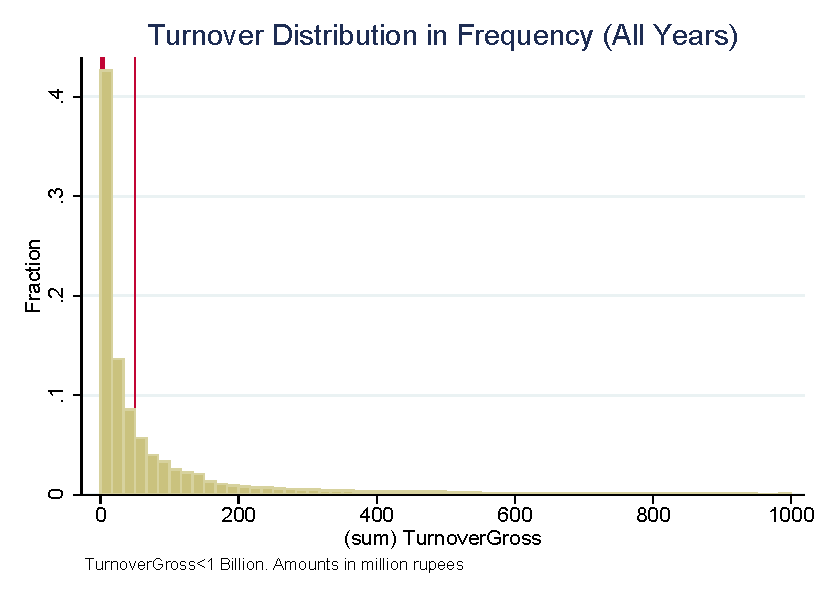
\includegraphics[width=1\textwidth]{graphs/TurnoverDistribution_Fraction_WeaklyPositive} 
\par\end{centering}
{\footnotesize{}{}{}Notes: }{\footnotesize \par}
\end{figure}

\newpage{}

\begin{figure}[t]
\caption{Firm Revenue Distribution at the Low Threshold}

\label{fig:LowestThreshold} 
\begin{centering}
\begin{tabular}{cc}
\vspace{0.2cm}
  & \vspace{0.2cm}
 \tabularnewline
\textbf{A: Bunching in Year 1}  & \textbf{B: Bunching in Year 2}\tabularnewline
b = 0.5  & b = 0.28\tabularnewline
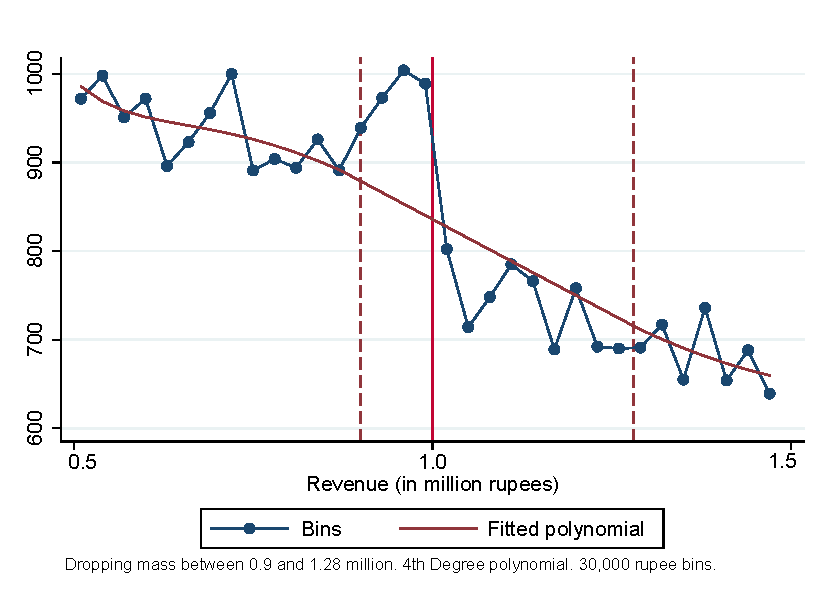
\includegraphics[width=0.4\textwidth]{graphs/BunchingYear1_1Million_Degree4_30000}  & 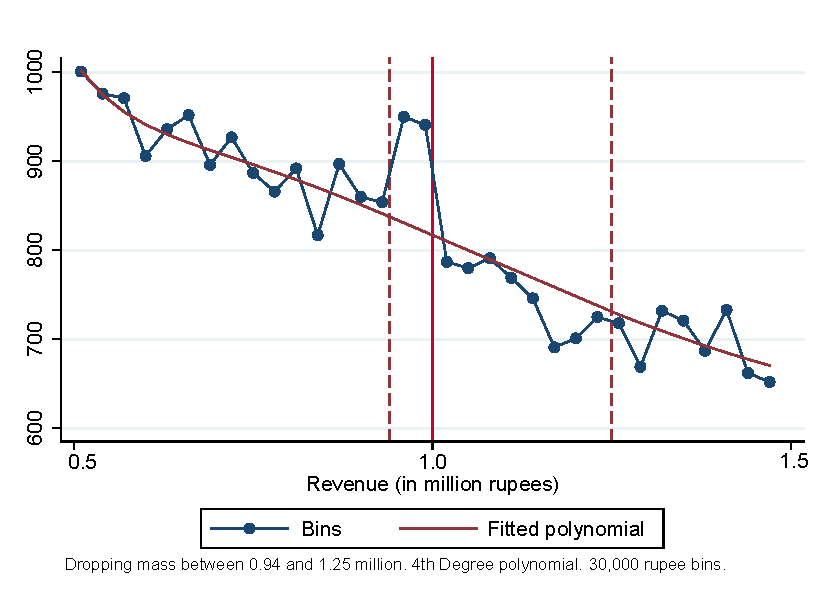
\includegraphics[width=0.4\textwidth]{graphs/BunchingYear2_1Million_Degree4_30000}\tabularnewline
\vspace{0.2cm}
  & \vspace{0.2cm}
 \tabularnewline
\textbf{C: No Bunching in Year 3}  & \textbf{D: No Bunching in Year 4}\tabularnewline
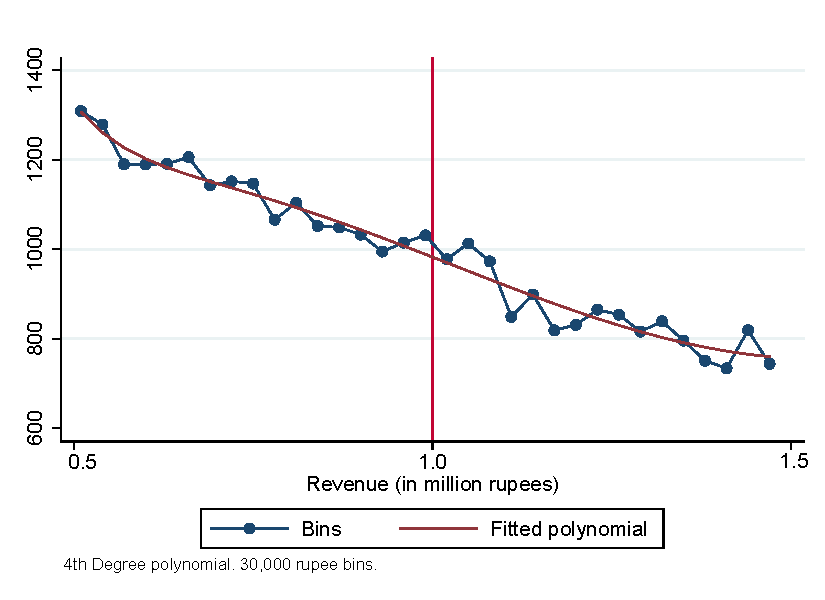
\includegraphics[width=0.4\textwidth]{graphs/BunchingYear3_1Million_Degree4_30000}  & 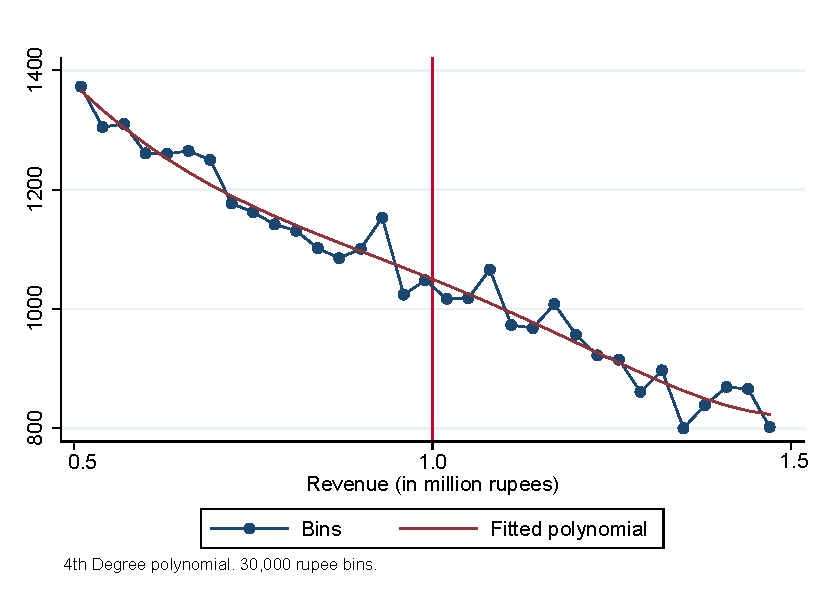
\includegraphics[width=0.4\textwidth]{graphs/BunchingYear4_1Million_Degree4_30000}\tabularnewline
\vspace{0.2cm}
  & \tabularnewline
\textbf{E: No Bunching in Year 5}  & \tabularnewline
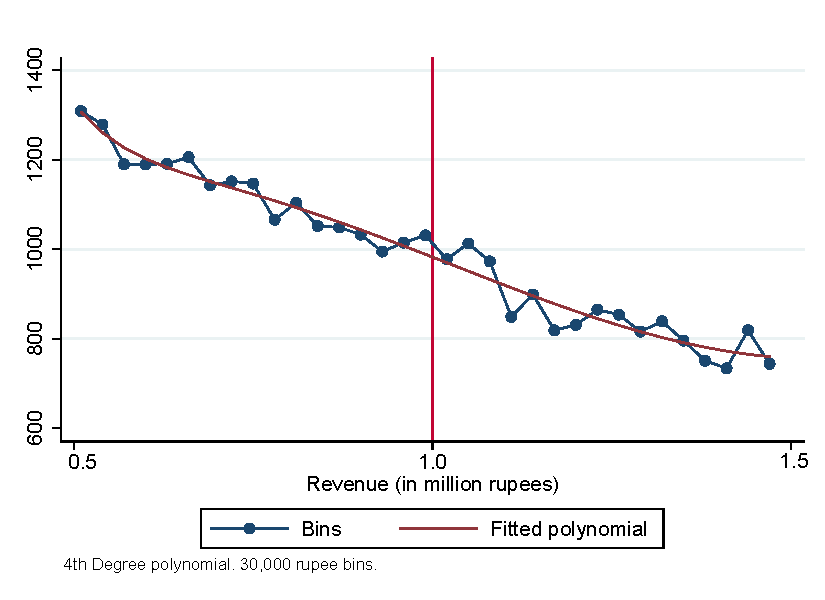
\includegraphics[width=0.4\textwidth]{graphs/BunchingYear3_1Million_Degree4_30000}  & \tabularnewline
\end{tabular}
\par\end{centering}
{\footnotesize{}{}{}Notes: }{\footnotesize \par}
\end{figure}

\newpage{}

\begin{figure}[t]
\caption{Firm Revenue Distribution at the Middle Threshold}

\label{fig:MiddleThreshold} 
\begin{centering}
\begin{tabular}{cc}
\vspace{0.2cm}
  & \vspace{0.2cm}
 \tabularnewline
\textbf{A: Bunching in Year 1}  & \textbf{B: Bunching in Year 2}\tabularnewline
b = 0.34  & b = 0.43\tabularnewline
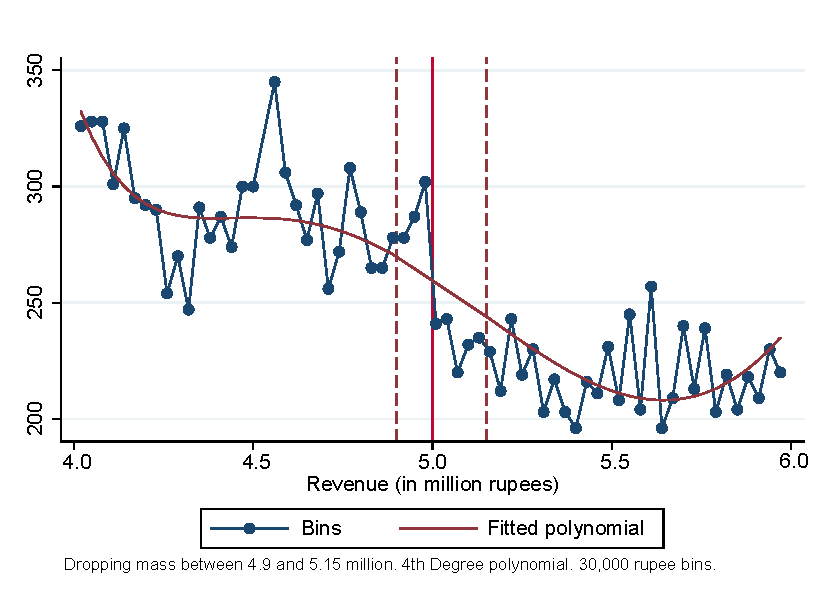
\includegraphics[width=0.4\textwidth]{graphs/BunchingYear1_5Million_Degree4_30000}  & 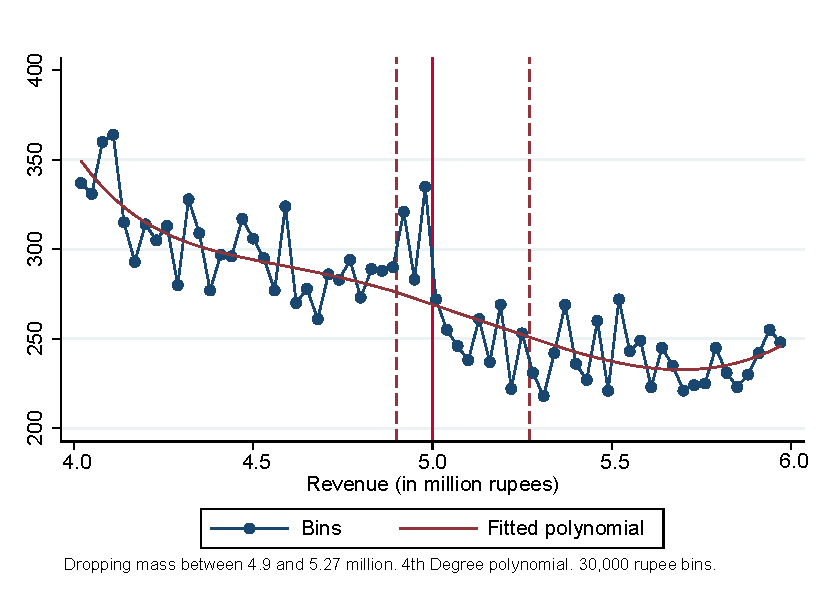
\includegraphics[width=0.4\textwidth]{graphs/BunchingYear2_5Million_Degree4_30000}\tabularnewline
\vspace{0.2cm}
  & \vspace{0.2cm}
 \tabularnewline
\textbf{C: No Bunching in Year 3}  & \textbf{D: No Bunching in Year 4}\tabularnewline
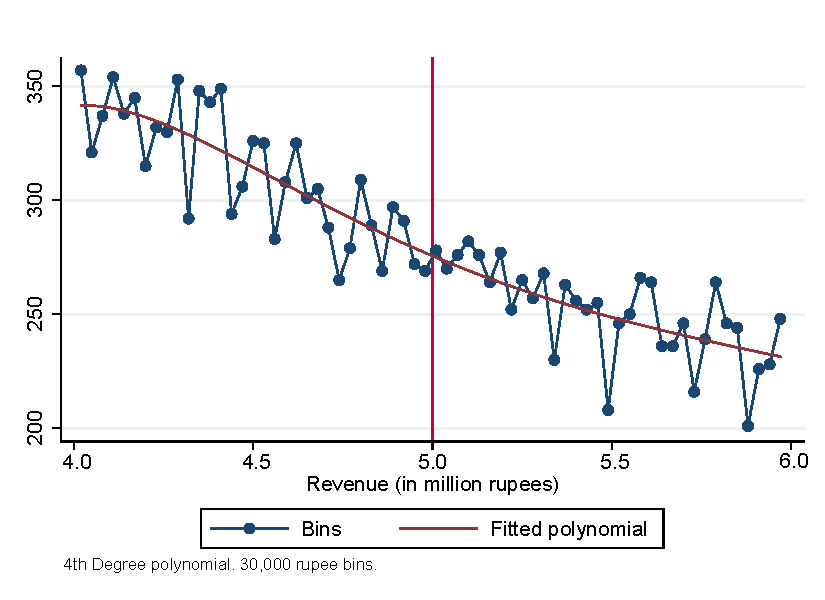
\includegraphics[width=0.4\textwidth]{graphs/BunchingYear3_5Million_Degree4_30000}  & 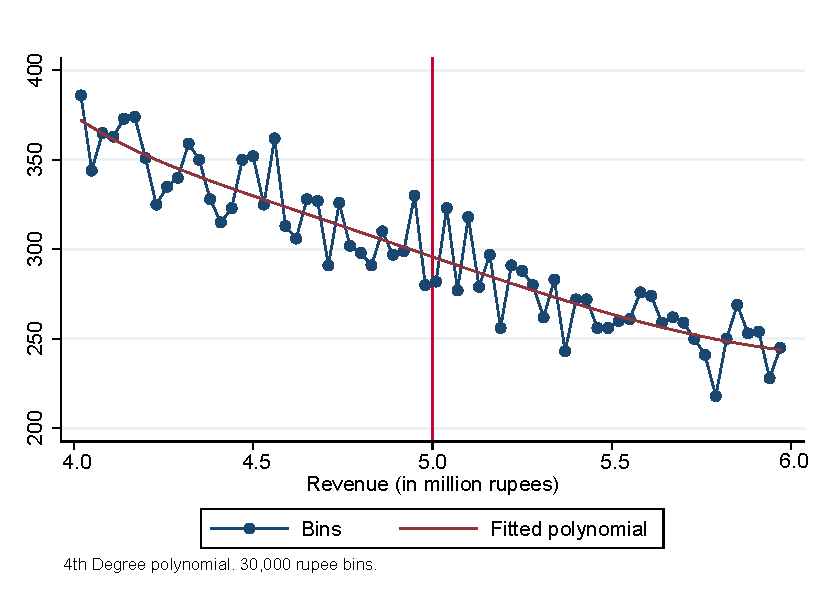
\includegraphics[width=0.4\textwidth]{graphs/BunchingYear4_5Million_Degree4_30000}\tabularnewline
\vspace{0.2cm}
  & \tabularnewline
\textbf{E: No Bunching in Year 5}  & \tabularnewline
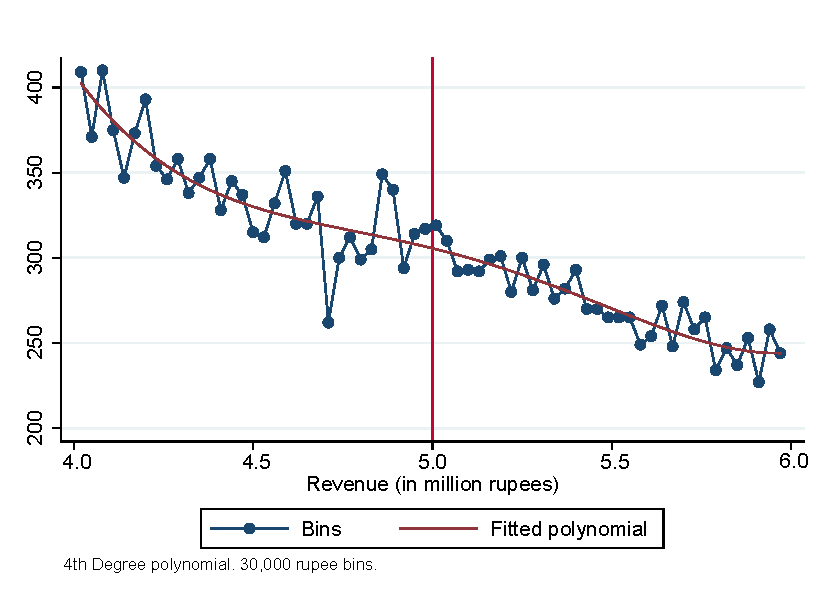
\includegraphics[width=0.4\textwidth]{graphs/BunchingYear5_5Million_Degree4_30000}  & \tabularnewline
\end{tabular}
\par\end{centering}
{\footnotesize{}{}{}Notes: }{\footnotesize \par}
\end{figure}

\newpage{}

\begin{figure}[t]
\caption{Firm Revenue Distribution at the High Threshold}

\label{fig:HighestThreshold} 
\begin{centering}
\begin{tabular}{cc}
\vspace{0.2cm}
  & \vspace{0.2cm}
 \tabularnewline
\textbf{A: Bunching in Year 1}  & \textbf{B: Bunching in Year 2}\tabularnewline
b = 2.6  & b = 2.98\tabularnewline
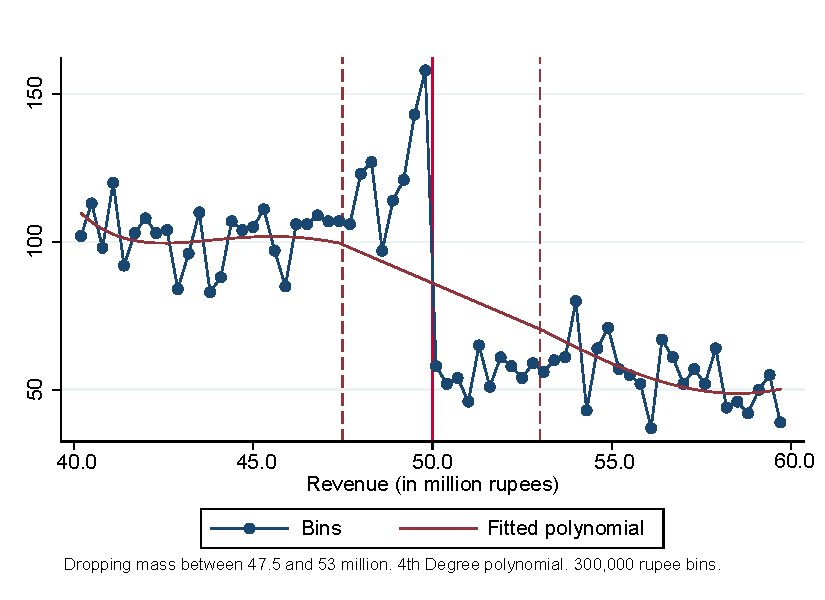
\includegraphics[width=0.4\textwidth]{graphs/BunchingYear1_50Million_Degree4_3lac}  & 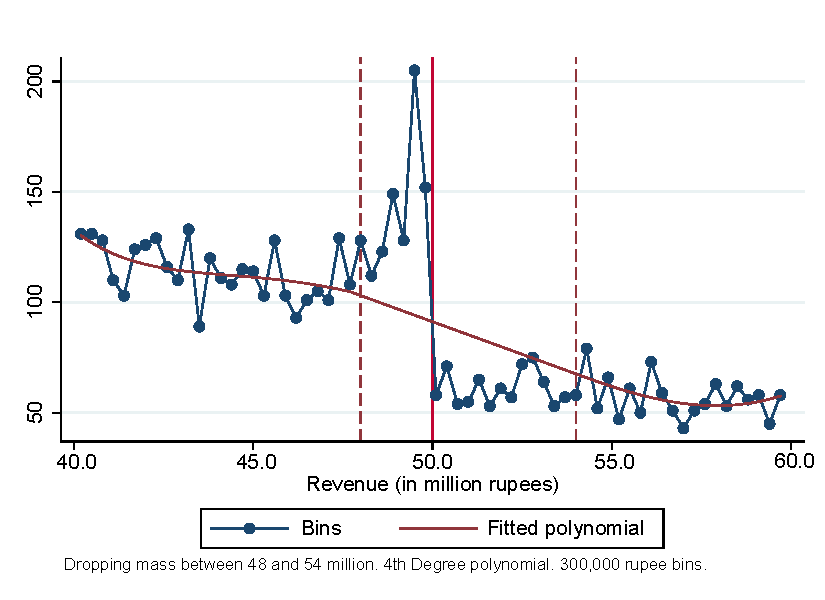
\includegraphics[width=0.4\textwidth]{graphs/BunchingYear2_50Million_Degree4_3lac}\tabularnewline
\vspace{0.2cm}
  & \vspace{0.2cm}
 \tabularnewline
\textbf{C: Bunching in Year 3}  & \textbf{D: No Bunching in Year 4}\tabularnewline
b = 1.87  & \tabularnewline
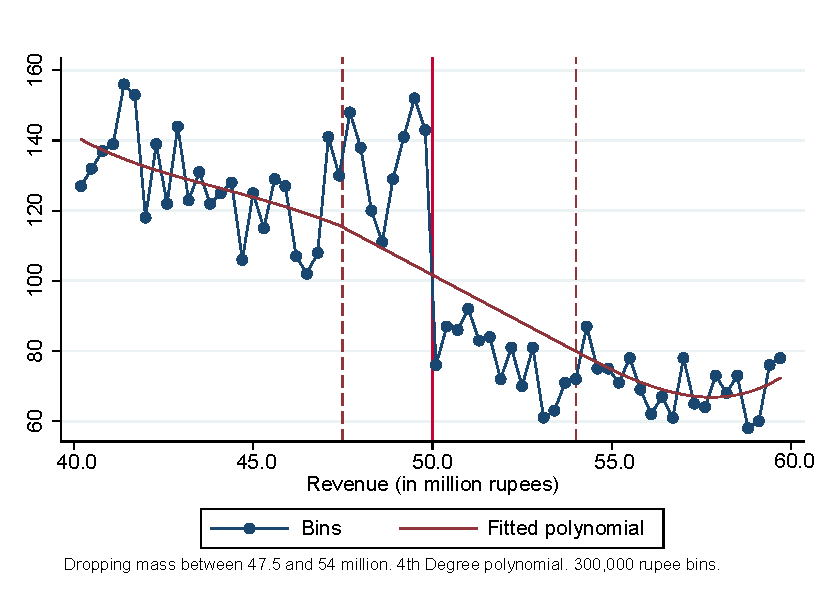
\includegraphics[width=0.4\textwidth]{graphs/BunchingYear3_50Million_Degree4_3lac}  & 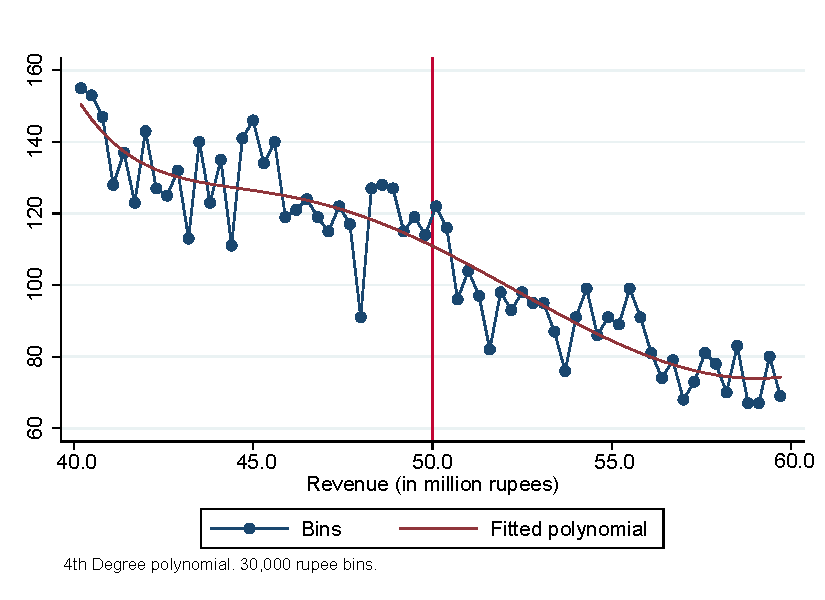
\includegraphics[width=0.4\textwidth]{graphs/BunchingYear4_50Million_Degree4_3lac}\tabularnewline
\vspace{0.2cm}
  & \tabularnewline
\textbf{E: No Bunching in Year 5}  & \tabularnewline
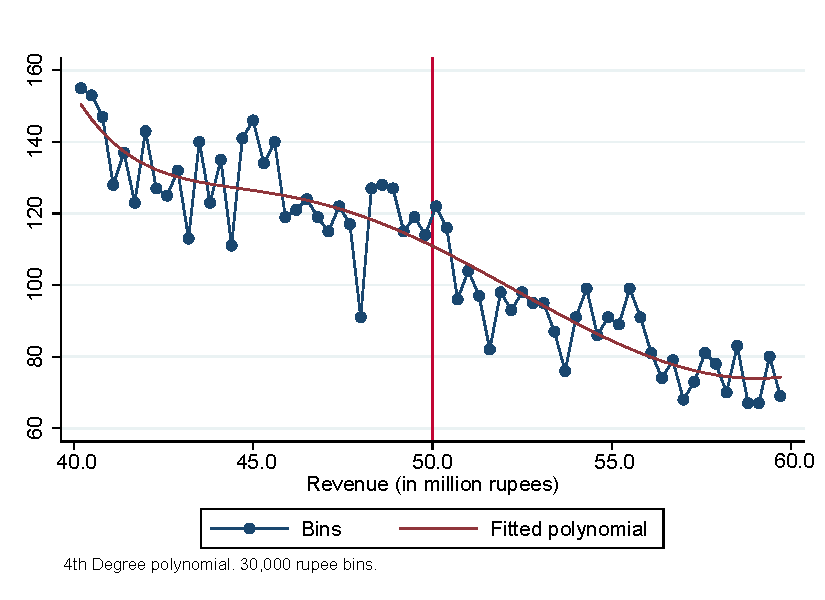
\includegraphics[width=0.4\textwidth]{graphs/BunchingYear4_50Million_Degree4_3lac}  & \tabularnewline
\end{tabular}
\par\end{centering}
{\footnotesize{}{}{}Notes: }{\footnotesize \par}
\end{figure}

\newpage{}

\begin{figure}[t]
\caption{Distribution of Compliance Costs by Revenue Size}

\label{fig:ComplianceCosts}\vspace{0.2cm}

\begin{centering}
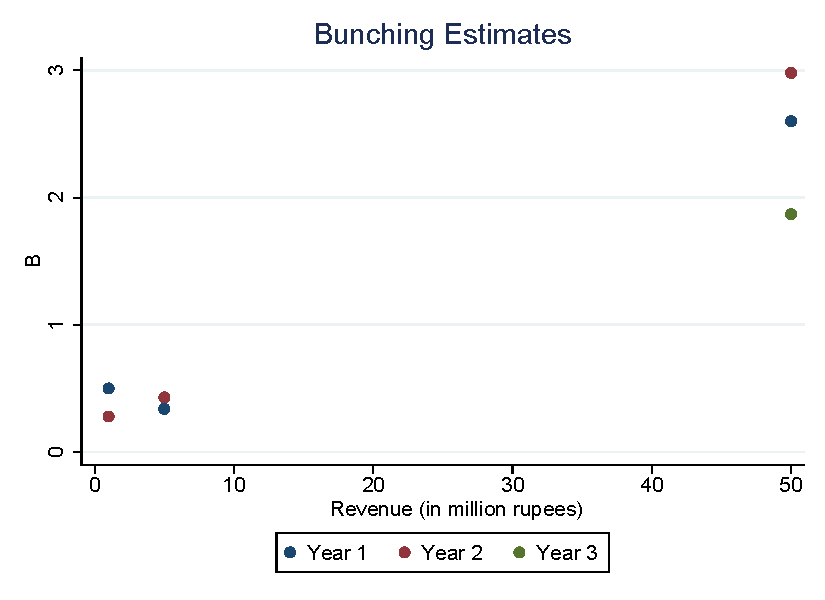
\includegraphics[width=1\textwidth]{graphs/BunchingEstimates} 
\par\end{centering}
{\footnotesize{}{}{}Notes: }{\footnotesize \par}
\end{figure}
                         %

\appendix
%Appendices
\chapter{Appendix ``VAT in Emerging Economies: Does Third Party Verification Matter?"}
%\addcontentsline{toc}{chapter}{Appendix}
%\begin{appendices}
%\appendix
%\counterwithin{figure}{section}
%\counterwithin{table}{section}
\section{Data Summary} \label[appendix]{sec:overall_analysis}
\begin{figure}[H]
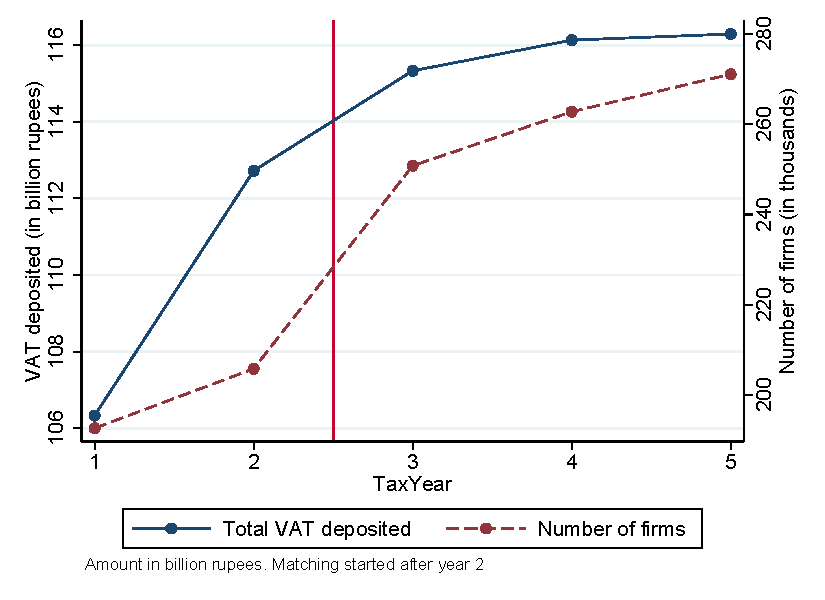
\includegraphics[width=.7\textwidth]{graphs/TotalVATDeposited_ALL_Real.pdf}
\caption{Total VAT remitted (for all firms), in real terms}  
\label{fig:vatdeposited-all}
\floatfoot{\scriptsize The third party verification policy began at the beginning of year 3. VAT remitted increases from \rupee 106.33 billion in year 1 to \rupee 116.29 billion in year 5. This is an average annual growth rate of 1.8\% in real terms as compared to a real state level GDP growth rate of about 5.7\% (Source:\citep{delhihandbook2015}). The y axis is in billion rupees, where 1\$ roughly equals \rupee 65.Values have been adjusted to year 1 price terms.}
\end{figure}


In this section, we describe the distribution of the firms registered in the Delhi VAT system. In \cref{fig:vatdeposited-all}, we plot the total VAT collections and the total number of firms registered for VAT across the 5 years. The third-party verification policy was implemented at the beginning of year 3. VAT deposits increase from \rupee 106.33 billion in year 1 to \rupee 116.29 billion in year 5. This is an average annual growth rate of 1.8\% in real terms as compared to a real state level GDP growth rate of about 5.7\%. We note that the number of registered firms go up sharply after the policy change which implies that average collections per firm actually decrease. We believe that this increase in the number of firms is driven by unrelated policy changes. Specifically, before quarter 2 of year three, firms had to deposit a surety amount between \rupee 50,000 to \rupee 100,000 as part of registration. The tax authority relaxed this restriction with the goal of improving ``ease of doing business'' from the second quarter of year three onwards.

\todo[inline,caption={Average Tax Deposited},color=green]{We should present average amount deposited in this graph. We decided not to do this.}

\begin{figure}[h] 
\centering
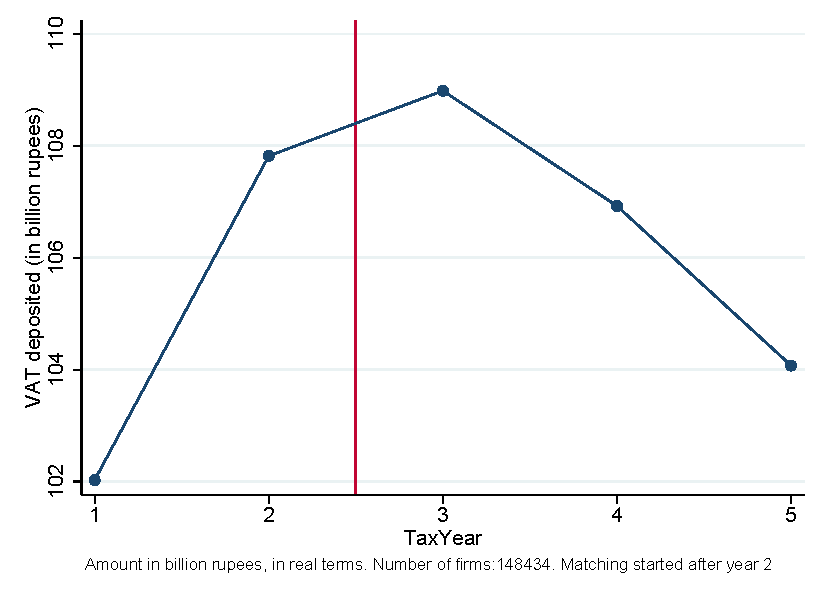
\includegraphics[width=.7\textwidth]{graphs/TotalVATDeposited_TotalCount5_Real.pdf}
\caption{Total VAT remitted (for firms that are present in all years)}
\floatfoot{\scriptsize Total collection trends for firms that are present in all the years of our sample period. There are 148434 such firms. The y axis is in billion rupees, where 1\$ roughly equals \rupee 65. Values have been adjusted to year 1 price terms. VAT remitted increases from \rupee 102.02 billion in year 1 to \rupee 104.07 billion in year 5.}
\label{fig:vatdeposited-alwayspresent}
\end{figure}

The number of firms filing a return increases from 192,664 in year 1 to 271,090 in year 5. There is a wide variation in the amount deposited. To begin with, only about 50\% of registered firms remit a positive VAT in any given filing period. Further, between 7 and 15\% of the firms (depending upon the tax period) that file a return report a zero turnover (sales). Furthermore, between 5 and 9\% of the firms declare their entire turnover to consist of interstate (or non-local) sales and about 32\% firms declare their entire turnover to be purely local
(refer to \Cref{tbl:all-summary}). Note that the third party verification mechanism breaks down for inter-state sales since the transacting firm's returns are submitted to a different tax authority and to date there has been little coordination between different tax jurisdictions on such cross-checking.\footnote{The GST bill legislated
by the central and state governments will unify the tax administration and make it much easier to cross-check inter-state transactions.} 

\begin{figure}[H]
\scriptsize
\centering
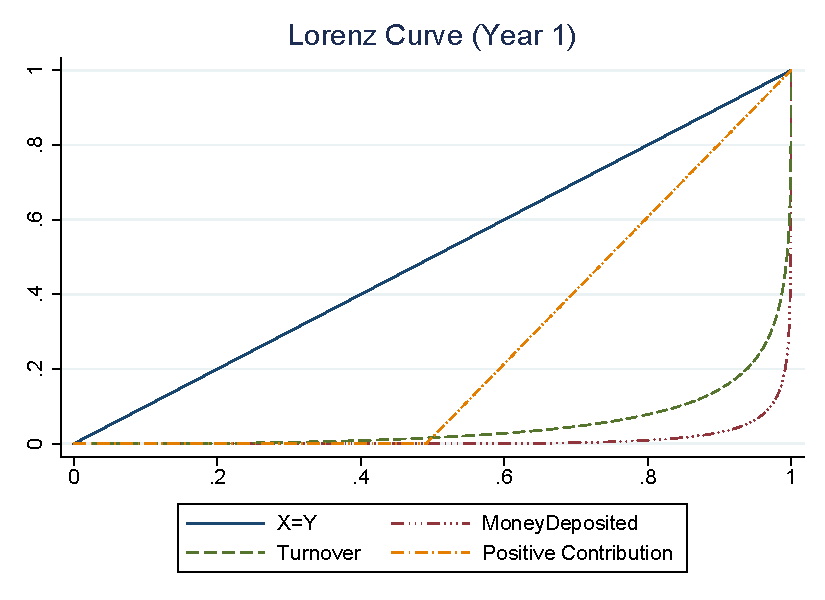
\includegraphics[width=.7\textwidth]{graphs/LorenzCurve_TaxYear1.pdf}
\caption{Lorenz Curve for all firms in Tax Year 1}
\label{fig:lorenzyear1}
\floatfoot{Note: Only 50\% of firms deposit any taxes, and 5\% of firms provide 95\% of total collections. Lorenz curve for all the firms in year 1 of our dataset (returns collated at annual level).}
\end{figure}

\todo[inline,caption={Thought}, color=green]{I guess if even before the policy 5\% of firms generated 95\% of the revenues, it's not so surprising that perhaps after policy the main increase comes from  them. Or perhaps we should say that even after policy we see that the tax base does not expand. \textbf{AM}: This true. I am not sure
where we should say this }

\begin{table}[h]
\footnotesize
%\scriptsize
\begin{threeparttable}
\begin{tabular}{lcccccc}\\ 
\hline \hline
(1)&(2)&(3)&(4)&(5)&(6)&(7)\\
Year & No. of Firms & VAT Remitted & \% Positive VAT  & \% Zero-Turnover  & \% Interstate & \% Local Firms \\  
& & & Deposited Firms & Firms &Firms & \\ \hline
1&192664& 106330.3 &50.88&7.10&9.03&31.26 \\
2&205832&112720.1&48.72&9.51&7.72&31.40 \\
3&250805&115330.6&47.57&15.05&5.94&31.68 \\
4&262775&116132.1&49.70&13.68&5.70&32.70 \\
5&271090&116292.4 &53.60&13.98&6.00&32.64 \\ \hline \hline
\end{tabular} 
\begin{tablenotes}[para,flushleft]
\scriptsize
Summary of all the firms that filed a return in the given year. Column (3) shows total VAT collected by the tax authority from all firms in that year in million rupees, with \rupee 65 approximately equal to \$1. Column (4) shows percentage of firms that deposited a positive amount of VAT. Column (5) show percentage of firms which filed a return but declared a turnover of zero. Column (6) shows percentage of firms that had a non-zero turnover and entire sales were interstate. Column (7) shows percentage of firms who had a non-zero turnover and all sales were local. For example, in year 1, 31.26\% firms had only local sales, 9.03\% had only interstate sales, and 7.1\% had a turnover of 0. Therefore, roughly 53\% of the firms had a non-zero turnover and had declared both local as well as inter-state sales.
\end{tablenotes}
\caption{Summary stats: All firms}
\label{tbl:all-summary}
\end{threeparttable}
\end{table}

In \cref{fig:lorenzyear1,fig:lorenzyear5} we plot Lorenz curves for (a) total turnover, (b) VAT remitted, and (c) a dummy for any positive VAT remitted separately for year 1 and 5 of the study. Inequality in contributions is stark with the top 5\% of firms remitting roughly 95\% of the total VAT collected by the tax authority. The number of firms that remit any VAT is surprisingly low, with the number hovering around 50\% across the 5 years.

\begin{figure}[h]
\scriptsize
\centering
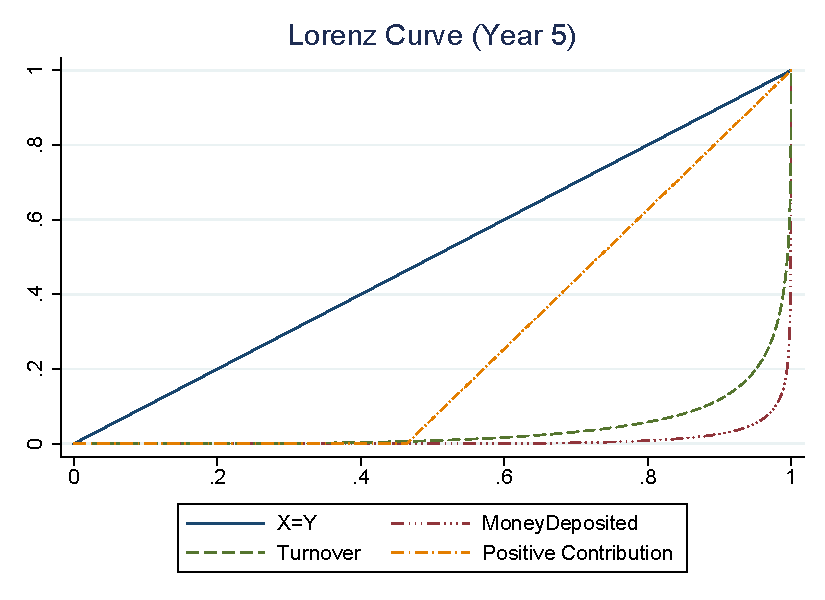
\includegraphics[width=.7\textwidth]{graphs/LorenzCurve_TaxYear5.pdf}
\caption{Lorenz Curve for all firms in Tax Year 5}
\label{fig:lorenzyear5}
\end{figure}

In \cref{fig:vatdeposited-alwayspresent} we focus our attention on firms which are present in all 5 years of our dataset i.e. we drop firms that enter or exit during our time-frame of interest. There are 148,434 such firms which remit roughly 95\% of our total tax collections in year 1 and 89\% of the tax collections in year 5. VAT
remits from these firms go from \rupee 102.02 billion in year 1 to \rupee 104.07 billion in year 5 (for a real growth rate of 0.39\%). In this set of firms, the percentage of firms remitting a positive amount goes up marginally, compared to all firms, to about 57\%. The percentage of firms that declare a turnover of zero is
between 2.5 to 8.5\% across the 5 years. The percentage of firms doing only interstate sales and only local sales is also comparable to the entire sample (refer to \cref{tbl:always_summary}). To conclude, our estimation sample comprises the bulk of the tax collections for the state throughout the study period. 

\todo[inline,caption={AM: Point of Appendix A?}, color=green]{We need to have some point when we describe statistics in the text. What is the point of telling people about the fraction of inter-state sales etc.? \textbf{We now refer to Appendix A in the summary statistics section}}



\begin{table}[h]
\footnotesize
%\scriptsize
\begin{threeparttable}
\begin{tabular}{cccccc}\\ \hline \hline
(1)&(2)&(3)&(4)&(5)&(6)\\
Year & VATDeposited & \% Positive VAT  & \% Zero-Turnover & \% Interstate & \% Local Firms \\  
& & Deposited Firms & Firms &Firms & \\ \hline
1& 102024.5 &54.60&2.50&6.97&30.76 \\
2&107820.3 &54.09&3.09&5.95&31.14 \\
3&108985.1 &57.20&3.88&5.34&30.61 \\
4&106926.4&57.50&5.35&5.18&30.45 \\
5&104071.8 &60.49&8.50&5.22&29.74 \\ \hline \hline
\end{tabular} 
\begin{tablenotes}[para,flushleft]
  Summary of firms that filed a return in all the 5 years for which we have the data (2010-11 to 2014-15). Number of such firms in our sample is 148434. Column (2) shows total VAT remitted by the tax authority from all firms in that year in million rupees, with \rupee 65 approximately equal to \$1. Column (3) shows percentage of firms that remitted a positive amount of VAT. Column (4) show percentage of firms which filed a return but declared a turnover of zero. Column (5) shows percentage of firms that had a non-zero turnover and entire sales were interstate. Column (6) shows percentage of firms who had a non-zero turnover and all sales were local. For example, in year 1, 30.76\% of the 148434 firms that are present in all the years of our sample, had only local sales, 6.97\% had only interstate sales, and 2.5\% had a turnover of 0. Therefore, roughly 60\% of the firms had a non-zero turnover and had declared both local as well as inter-state sales.
\end{tablenotes}
\caption{Summary stats: Always present firms}
\label{tbl:always_summary}
\end{threeparttable}
\end{table}


\pagebreak


\section{Quarterly Results}
\label[appendix]{sec:quarterlyresults}

\begin{figure}[t] 
\caption{Wholesalers vs Retailers: Quarterly trends (in real terms) with confidence intervals}
\label{fig:group1-pretrends-quarterly}
\centering
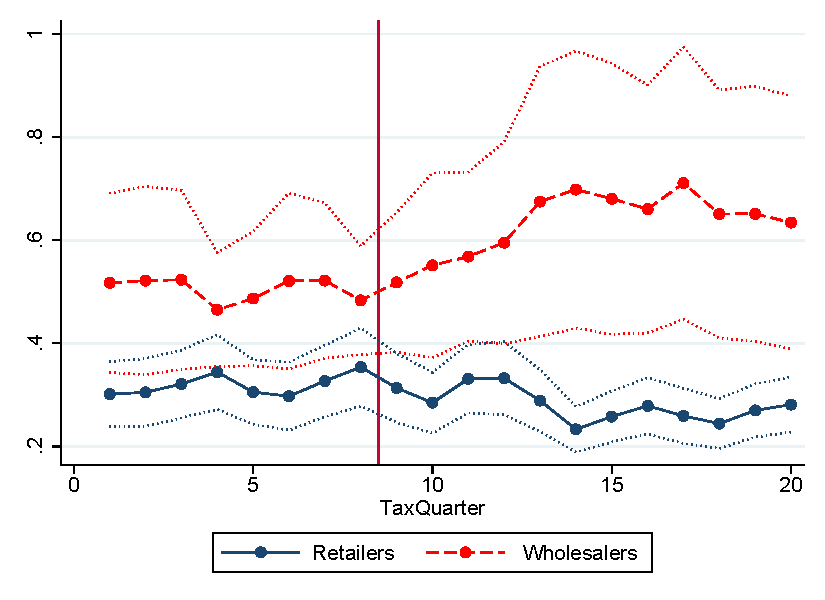
\includegraphics[width=.8\textwidth]{graphs/MeanMoneyDeposited_quarterly_with_confidenceintervals_Real.pdf}
\floatfoot{\footnotesize $N_W=11482$, $N_R=15337$. VAT remitted is in million rupees, with \rupee 65 approximately equal to \$1. VAT remitted has been inflation adjusted to Q1-2010-11 price levels. Sample smaller than the annual frequency sample because in year 1 and year 2 firms with turnover less than 5 million had to file at annual or semi-annual frequency.}
\end{figure}

\pagebreak
\subsection{Quarterly Analysis Along with Falsification Test}
\label[appendix]{subsec:falsification-test}
In addition to the basic model explained in \cref{subsec:identification_model}, we carry out robustness check by the falsification test described below. In \cref{eq:basic}, we now add a $Pre_{it}$ dummy which is equal to 1 if the quarter is 7 or 8 i.e. just before the introduction of the third party verification policy. We also interact the $Pre_{it}$ dummy with $\mathbb{I}\{\text{Wholesaler}_{i}\}$ which is a dummy for the firm i being a wholesaler. The falsification test is provided by coefficient $\mu$ corresponding to the interaction between $Pre_{it}$ dummy and $\mathbb{I}\{\text{Wholesaler}_{i}\}$ dummy. The coefficient indicates whether, before the introduction of the policy, the outcome variable is evolving similarly between wholesalers and retailers during the 2 quarters before the introduction of the policy. Consistent with the quarterly event-study analysis (\cref{fig:eventstudy-figure-quarter}), the pre-policy effect on wholesalers is close to zero, precisely estimated,\footnote{The standard errors are smaller than those for $\gamma$ coefficient.} and statistically insignificant. Results shown in \cref{tbl:event-falsification-table}.

\begin{multline} \label{eq:falsification}
 y_{it}=\alpha_i+\nu_t+\beta*Post_{it}+\delta*Pre_{it}+\gamma*Post_{it}*\mathbb{I}\{\text{Wholesaler}_{i}\} \\
  +\mu*Pre_{it}*\mathbb{I}\{\text{Wholesaler}_{i}\}+\epsilon_{it}
\end{multline}

\scalebox{0.9}{
\begin{threeparttable}
\centering 
\footnotesize
\caption{Falsification test: Wholesalers and Retailers (Quarterly, in real terms)}
\label{tbl:event-falsification-table}
 \begin{tabular}{lccccc} \hline \hline
     & (1) & (2) & (3) & (4) & (5)  \\
VARIABLES & Positive VAT  & VAT Remitted & Tax Credit & Output Tax & Output Tax -\\
   & Remitted &  &  & & Tax Credit\\ \hline
Post*Wholesaler & -0.0147*** & 0.158*** & -0.0240 & 0.132*** & 0.156*** \\
 & (0.00355) & (0.0491) & (0.0496) & (0.0392) & (0.0501) \\
PrePolicy*Wholesaler & -0.00278 & -0.0312 & 0.0385 & 0.00530 & -0.0332 \\
 & (0.00372) & (0.0304) & (0.0308) & (0.0269) & (0.0320) \\
\hline
Post & 0.0139***  & -0.0604* & 0.0382* & -0.0194 & -0.0576** \\
 & (0.00349)  & (0.0322) & (0.0220) & (0.0392) & (0.0289) \\
PrePolicy & 0.0189***  & 0.0288 & 0.0637*** & 0.0928*** & 0.0291 \\
 & (0.00352) & (0.0210) & (0.0240) & (0.0359) & (0.0201) \\
\hline
Mean Dep.Var. & 0.44 & 0.52 & 0.54 & 1.02 & .48 \\
&(0.00)& (0.09)&(0.15)&(0.22)&(0.09) \\ \hline
Observations & 536,380 & 536,380 & 536,380 & 536,380 & 536,380 \\
R-squared & 0.549 & 0.86 & 0.78 & 0.96 & 0.86 \\ 
Number of Firms & 26,819 & 26,819 & 26,819 & 26,819 & 26,819 \\ \hline \hline
\end{tabular}
  \begin{tablenotes}[para,flushleft]
\footnotesize Robust standard errors in parentheses, clustered at firm level. $N_W=11482$, $N_R=15337$. Monetary amounts are in million rupees, inflation adjusted to price levels of Q1 of 2010-11, with \rupee 65 approximately equal to \$1. Column (1) shows linear probability regression of the probability of remitting a positive amount. Column (2)-(4) respectively show regression of the mean VAT remitted by firms, of the input tax credit claimed by firms, and the output tax collected by firms. To address the concern that VAT remitted has a significant mass at zero, column(5) shows regression of the difference between output tax and input credit declared by firms. Dependent variables have been price adjusted in Q1 of 2010-11 terms. Row ``Mean Dep.Var.'' shows mean and standard errors for wholesalers in quarter 1. *** p$<$0.01, ** p$<$0.05, * p$<$0.1
\end{tablenotes}
\end{threeparttable}}


\pagebreak

\section{Flexible DID Specifications}
\label[appendix]{sec:eventstudy-analysis}

\subsection{Econometric model of event study analysis}
\label[appendix]{subsec:eventstudy-econometrics}
We can take advantage of the large N and moderate T dimensions in our data set to estimate richer treatment effect models. In particular, we can examine flexibly the differential evolution of outcomes between wholesalers and retailers over the entire time-period under study. In particular, we estimate \cref{eq:flex} as outlined in
\cref{subsec:identification_model}. We normalize $\gamma_2$ in that equation ($\gamma_8$ for quarterly analysis) to zero so that the coefficients $\{\gamma_s\}_{s \in S }$ measure differential changes in the outcome and relative to the year (quarter) prior to the policy introduction.

We report the coefficients in graphical form, with their corresponding 95\% confidence intervals (see for example \cref{fig:eventstudy-figure-annual}). If the coefficients $\{\gamma_s\}_{s>2}$ (i.e., the coefficients after the introduction of the third party verification) are positive, that implies that outcomes increase on average for wholesalers relative to retailers after the policy introduction. If $\gamma_s$ is positive only for some $2 < s \leq \bar{s} \leq 5$, then the increase in outcomes is transitory, lasting up to $\bar{s}$ years after the policy introduction. If the coefficient $\gamma_1$ (i.e., the coefficient in the figure to the left of the policy introduction) is positive, then the outcome variable was declining  before the introduction of the policy. 

To formally test the hypothesis that pre-policy trends between wholesalers and retailers are not different, we test the null hypothesis $\gamma_1=\gamma_2=..=\gamma_{l-1}=0$ where l denotes the time period in which the automatic third party verification policy was introduced. For the analyses below (carried out for the quarterly and annual frequencies) we cannot reject that pre-treatment trends are equal between wholesalers and retailers.  

%\pagebreak


\begin{table}[h]
\footnotesize
\begin{threeparttable}
\begin{tabular}{lllll} \hline \hline
 & (1) & (2) & (3) & (4) \\
VARIABLES & Annual & Quarter & Top Decile &Top Decile  \\ 
 &  &  & (Annual) & (Quarter)  \\ \hline
Positive VAT Deposited & 0.68  & 0.27 & 0.02 &0.00 \\
VAT Deposited & 0.61 &  0.20 & 0.46 &0.27 \\
Tax Credit & 0.12 & 0.36 & 0.69 & 0.43 \\
Output Tax & 0.23 & 0.65 & 0.98 & 0.28 \\
Output Tax - Tax Credit & 0.56 & 0.54 & 0.56 & 0.69 \\ \hline
\end{tabular}
\begin{tablenotes}[para,flushleft]
To formally test the hypothesis that pre-policy trends between wholesalers and retailers are not different, we test the null hypothesis $\gamma_1=\gamma_2=..=\gamma_{l-1}=0$ where l denotes the time period in which the automatic third party verification policy was introduced. l is 3 in column (1) and (3), and 9 in column (2) and (4). Column (1) does the test for returns data at annual frequency, column (2) does the test for returns at quarterly frequency, and column (3) and (4) do the test for returns data at annual and quarterly frequency but only for firms in the top decile (of both retailers and wholesalers) of VAT remitted in year/quarter 1.
\end{tablenotes}
\caption{Pre-trend analysis: Wholesalers vs Retailers}
\label{tbl:}
\end{threeparttable}
\end{table}

%\pagebreak

\subsection{Annual Analysis}
\label[appendix]{subsec:eventstudy-annual}
\begin{figure}[H]
\centering
\subfloat[VAT Deposited]{
  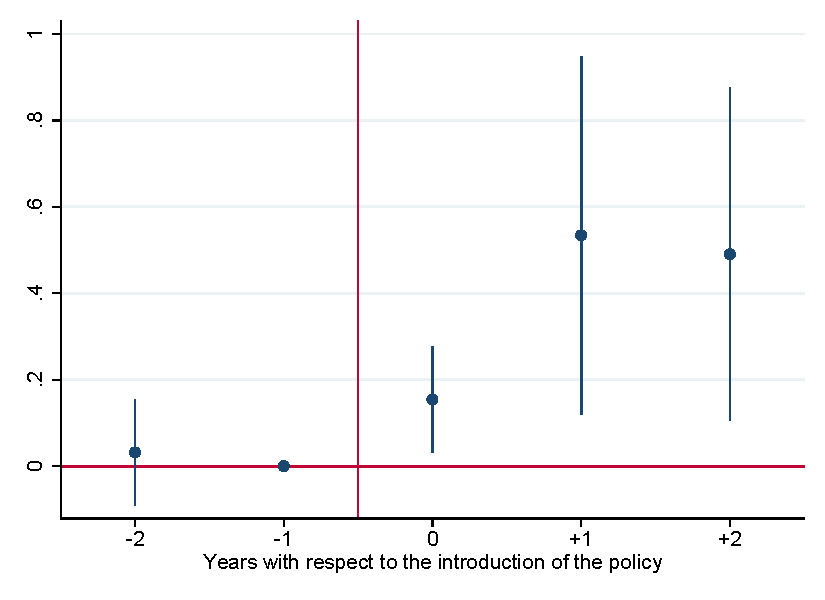
\includegraphics[width=55mm]{graphs/EventStudy-MoneyDeposited-Annual-Real.pdf}
  \label{fig:eventstudy-figure-annual-vatdeposited}
}
\subfloat[Output Tax - Input Credit]{
  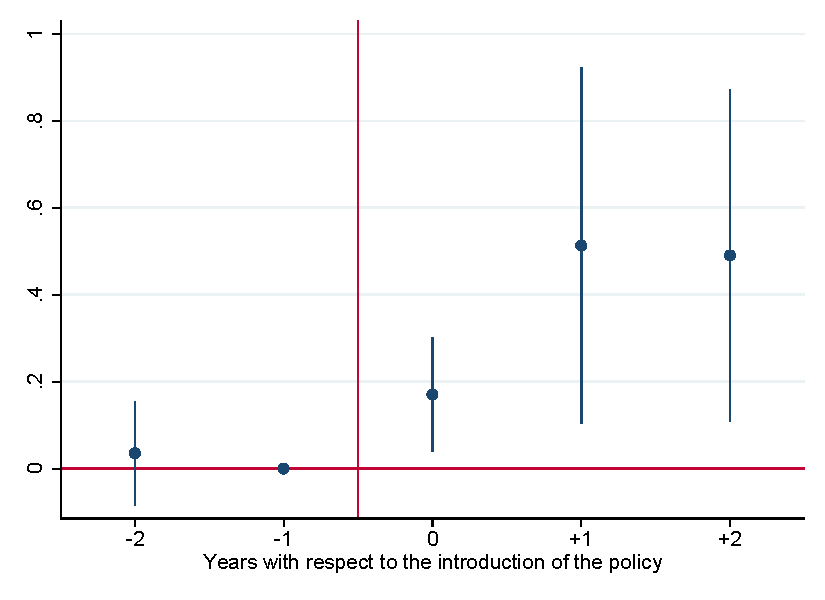
\includegraphics[width=55mm]{graphs/EventStudy-Diff-Annual-Real.pdf}
   \label{fig:eventstudy-figure-annual-diff}
}
\hspace{0mm}
\subfloat[Output Tax]{
  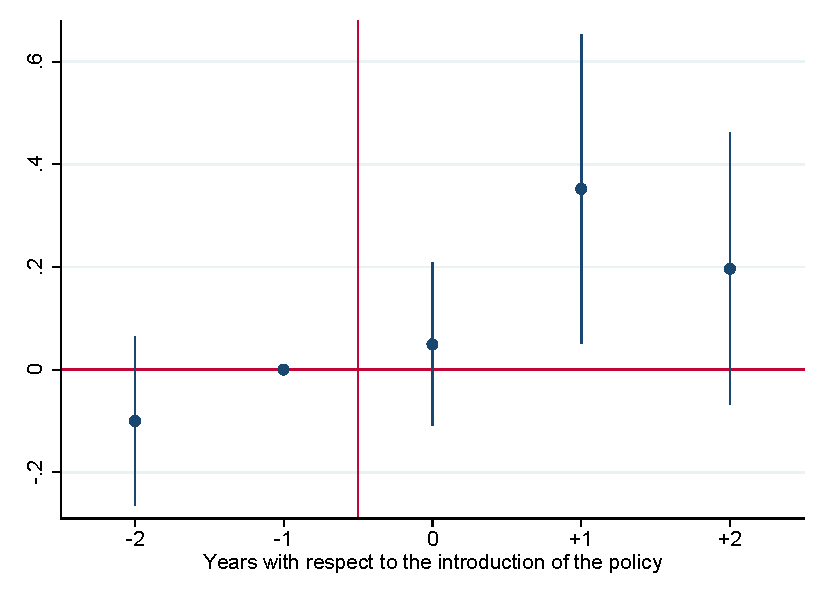
\includegraphics[width=55mm]{graphs/EventStudy-OutputTax-Annual-Real.pdf}
   \label{fig:eventstudy-figure-annual-outputtax}
}
\subfloat[Input Credit]{
  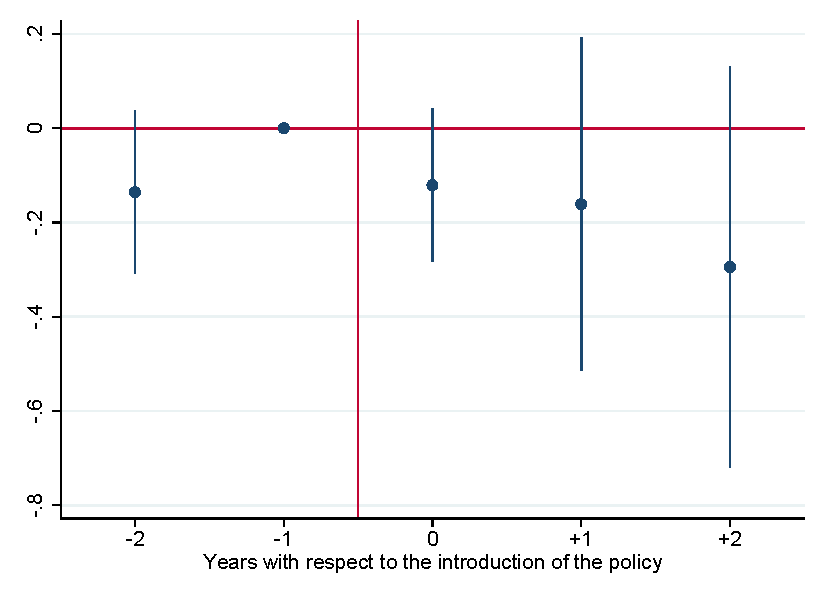
\includegraphics[width=55mm]{graphs/EventStudy-TaxCredit-Annual-Real.pdf}
   \label{fig:eventstudy-figure-annual-inputcredit}
}
\hspace{0mm}
\subfloat[Positive VAT Deposited]{   % ???
  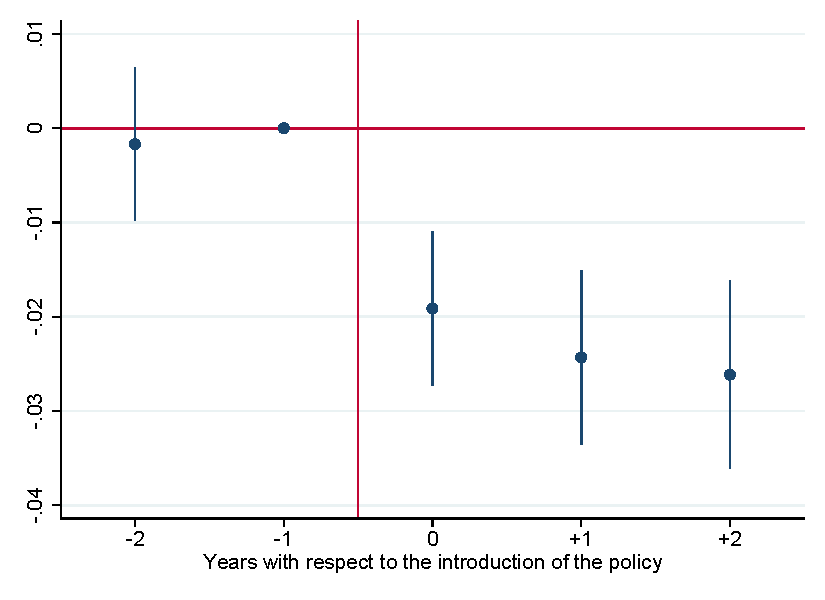
\includegraphics[width=55mm]{graphs/EventStudy-PositiveContribution-Annual.pdf}
   \label{fig:eventstudy-figure-annual-positivevat}
  }
\floatfoot{\footnotesize Notes: Graphical event-study analysis of the effect of third party verification policy on wholesalers compared to retailers. Confidence intervals were constructed with heteroskedasticity-robust standard errors, clustered at the firm level. The coefficient for the year ``-1'' (i.e., the year prior the policy) was normalized to zero. The regressions include firm fixed effects and time effects. The x axis indicates time, with annual observations and zero indicates the first year of the third party verification policy. Confidence intervals at the 95\% level. $N_W=32979$, $N_R=19515$. Coefficients in panel (a), (b), (c) and (d) are in million rupees with dependent variables price adjusted to the first year levels. \rupee 65 approximately equal to \$1. Pretrends are not statistically significant. }
\caption{Wholesalers vs Retailers: In Real Terms}
\label{fig:eventstudy-figure-annual}
\end{figure}


\subsection{Quarterly analysis}
\label[appendix]{subsec:eventstudy-quarter}

\begin{figure}[H]
\centering
\subfloat[VAT Deposited]{
  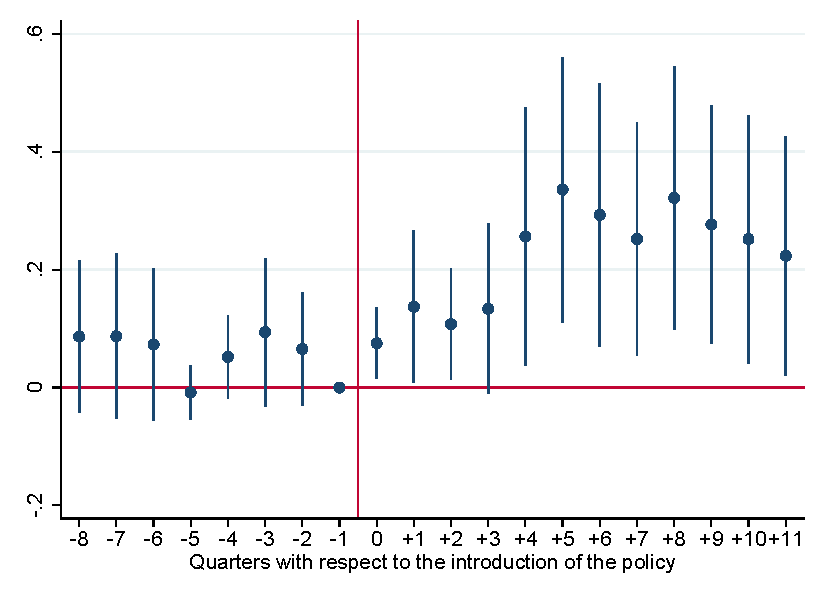
\includegraphics[width=55mm]{graphs/EventStudy-MoneyDeposited-Quarter-Real.pdf}
  \label{fig:eventstudy-figure-quarter-vatdeposited}
}
\subfloat[Output Tax - Input Credit]{
  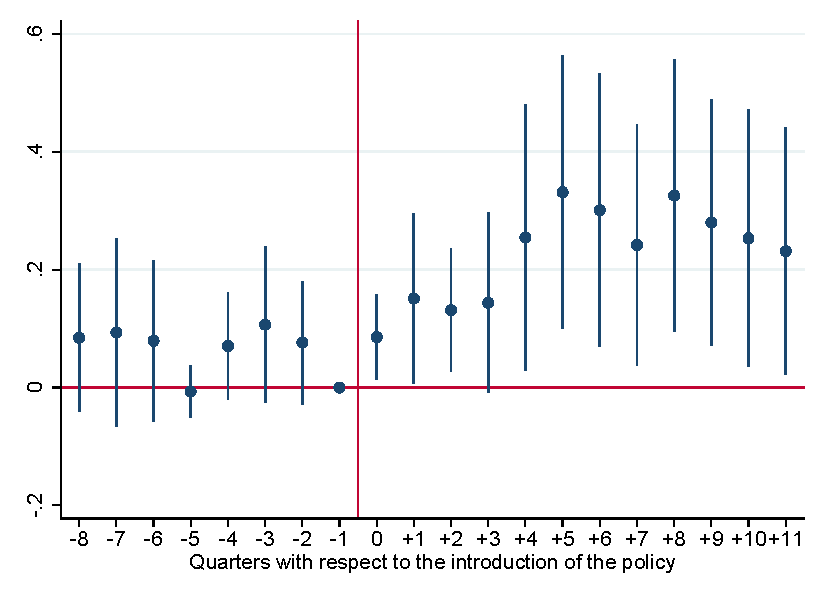
\includegraphics[width=55mm]{graphs/EventStudy-Diff-Quarter-Real.pdf}
   \label{fig:eventstudy-figure-quarter-diff}
}
\hspace{0mm}
\subfloat[Output Tax]{
  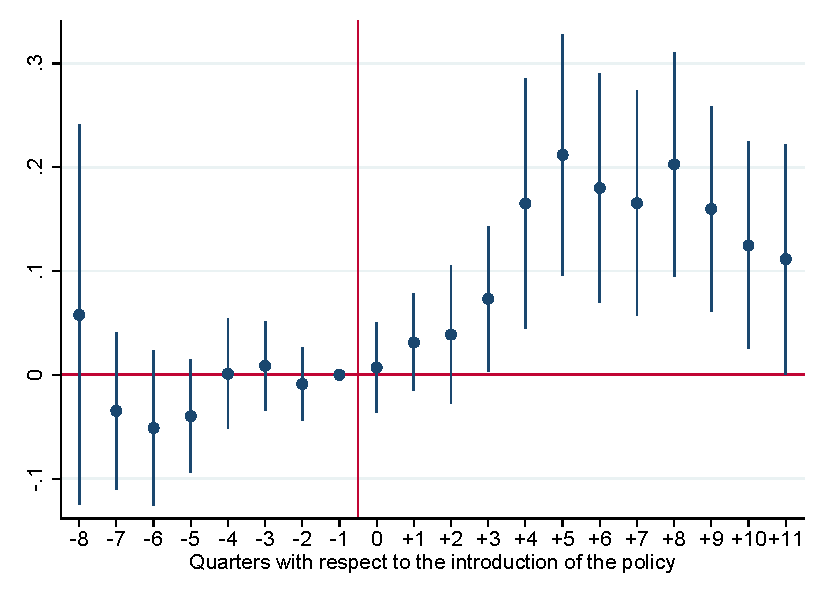
\includegraphics[width=55mm]{graphs/EventStudy-OutputTax-Quarter-Real.pdf}
   \label{fig:eventstudy-figure-quarter-outputtax}
}
\subfloat[Input Credit]{
  \includegraphics[width=55mm]{graphs/EventStudy-TaxCredit-Quarter-Real.pdf}
   \label{fig:eventstudy-figure-quarter-inputcredit}
}
\hspace{0mm}
\subfloat[Positive VAT Deposited]{   % ???
  \includegraphics[width=55mm]{graphs/EventStudy-PositiveContribution-Quarter.pdf}
   \label{fig:eventstudy-figure-quarter-positivevat}
  }
\floatfoot{\footnotesize Notes: Graphical event-study analysis of the effect of third party verification policy on wholesalers compared to retailers. Confidence intervals were constructed with heteroskedasticity-robust standard errors, clustered at the firm level. The coefficient for the quarter ``-1'' (i.e., the quarter prior to the policy) was normalized to zero. The regressions include firm fixed effects and time effects. The x axis indicates time, with quarterly observations and zero indicates the first quarter of the third party verification policy. Confidence intervals at the 95\% level. $N_W=11482$, $N_R=15337$. Coefficients in panel (a), (b), (c) and (d) are in million rupees with dependent variables price adjusted to the first quarter of 2010 levels. \rupee 65 approximately equal to \$1. Pretrends are not statistically significant.}
\caption{Wholesalers vs Retailers: In Real Terms}
\label{fig:eventstudy-figure-quarter}
\end{figure}

%\pagebreak

\section{Other Results}

\begin{figure}[H]
\centering
\subfloat[Output Tax - Input Credit]{
  \includegraphics[width=50mm]{graphs/HeterogeneityDiff_Real.pdf}
}
\subfloat[Output Tax]{
  \includegraphics[width=55mm]{graphs/HeterogeneityOutputTax_Real.pdf}
}
\hspace{0mm}
\subfloat[Input Credit]{
  \includegraphics[width=55mm]{graphs/HeterogeneityTaxCredit_Real.pdf}
}
\subfloat[Positive VAT Deposited]{   
  \includegraphics[width=55mm]{graphs/HeterogeneityPositiveContribution.pdf}
  }
\floatfoot{\footnotesize Notes: This figure plots the difference between wholesalers and retailers for different deciles, based on VAT remitted in the first year. The x axis indicates the decile. Confidence intervals at the 95\% level. Number of retailers is 32979 and number of wholesalers is 19515. Coefficients in panel (a), (b), and (c) are in million rupees, price adjusted to 2010-11 levels, with \rupee 65 approximately equal to \$1. Pretrends are not statistically significant.}
\caption{Heterogeneity Analysis: Wholesalers vs Retailers}
\label{heterogeneity-figure-annual}
\end{figure}
\pagebreak


\begin{figure}[H]
\centering
\subfloat[Output Tax - Input Credit]{
  \includegraphics[width=55mm]{graphs/EventStudy-Diff-Quarter_TopDecile_Real.pdf}
  \label{fig:eventstudy-figure-quarter-diff-topdecile}
}
\subfloat[Output Tax]{
  \includegraphics[width=55mm]{graphs/EventStudy-OutputTax-Quarter_TopDecile_Real.pdf}
  \label{fig:eventstudy-figure-quarter-outputtax-topdecile}
}
\hspace{0mm}
\subfloat[Input Credit]{
  \includegraphics[width=55mm]{graphs/EventStudy-TaxCredit-Quarter_TopDecile_Real.pdf}
    \label{fig:eventstudy-figure-quarter-inputcredit-topdecile}
}
\subfloat[Positive VAT Deposited]{  
  \includegraphics[width=55mm]{graphs/EventStudy-PositiveContribution-Quarter_TopDecile.pdf}
   \label{fig:eventstudy-figure-quarter-positivevat-topdecile}
  }
\floatfoot{\footnotesize Notes: Graphical event-study analysis of the effect of third party verification policy on wholesalers compared to retailers (for the top decile). Confidence intervals were constructed with heteroskedasticity-robust standard errors, clustered at the firm level. The coefficient for the group ``-1'' (i.e., the year prior the policy) was normalized to zero. The regressions include firm fixed effects and time effects. The x axis indicates time, with quarterly observations and zero indicates the first year of the third party verification policy. We have 20 quarters of data from 2010-11 to 2014-15. Confidence intervals at the 95\% level. Number of retailers is 1533 and number of wholesalers is 1148. Coefficients in panel (a), (b), (c) and (d) are in million rupees, price adjusted to Q1 of 2010-11 levels, with \rupee 65 approximately equal to \$1. Pretrends are not statistically significant.}
\caption{Quarterly Analysis for Top Decile: Wholesalers vs Retailers}
\label{fig:eventstudy-figure-quarter-topdecile}
\end{figure}



\section{Policy Execution: Other}
\label[appendix]{sec:execution}
%\setcounter{figure}{0}

\subsection{Difference-in-difference-in-difference: Proportion registered sales}
\label{subsec:ddd-rxprop}
\begin{figure}[H]
\centering
\subfloat[VAT Deposited]{
  \includegraphics[width=55mm]{graphs/DDD_VATDeposited_Real.pdf}
}
\subfloat[Output Tax - Input Credit]{
  \includegraphics[width=55mm]{graphs/DDD_Diff_Real.pdf}
}
\hspace{0mm}
\subfloat[Output Tax]{
  \includegraphics[width=55mm]{graphs/DDD_OutputTaxBeforeAdjustment_Real.pdf}
}
\subfloat[Input Credit]{
  \includegraphics[width=55mm]{graphs/DDD_TaxCreditBeforeAdjustment_Real.pdf}
}
\hspace{0mm}
\subfloat[Positive VAT Deposited]{   % ???
  \includegraphics[width=55mm]{graphs/DDD_PositiveContribution.pdf}
  }
\floatfoot{\footnotesize Notes: This figure plots the difference between wholesalers and retailers explained in \cref{eq:ddd}. The x axis indicates time, with quarterly observations and zero indicates the first quarter of the third party verification policy. Confidence intervals at the 95\% level. Number of retailers is 15337 and number of wholesalers is 11482. Coefficients in panel (a), (b), (c) and (d) are in million rupees, price adjusted to Q1 of 2010-11 levels. Pretrends are not statistically significant. }
\caption{Wholesalers vs Retailers}
\label[appendix]{ddd-figure-quarter}
\end{figure}


\subsection{Revisions}\label[appendix]{subsec:revisions}
\todo[inline,caption={Aprajit: Revisions}, color=green]{The point of this section is to show that revision behavior post-policy is consistent with collusion on the part of retailers. At the moment we see (a) \# revisions go up immediately post-policy but then are down again by the end of the study and (b) the top percentile of wholesalers and retailers have about the same number of changes in revisions post policy as do the top 10\%.  The DID, however, shows that retailers revised their returns more than the wholesalers. Further, we see that these revisions were as likely to lead to decreases in tax liabilities as increases in tax liabilities for retailers (relative to wholesalers).}

\begin{figure}[h] 
\centering
\includegraphics[width=0.75\textwidth]{graphs/RevisionTrends_All.pdf}
\caption{Mean revisions for all firms}
\label{fig:revision_all}
\end{figure}


Firms are allowed to revise filed returns until the end of next financial year. Before the start of the monitoring policy the average revision rates were around 13\% i.e. the mean of the total number of times a firm filed its returns was 1.13 (in Y1 and Y2). This revision rate was constant in the pre-period for both retailers and
wholesalers. However, immediately after the introduction of the policy, the revision rates shot up to 30\% i.e. the mean of the total number of returns filed by a firm was now 1.3 (in Y3). As the issue mentioned between the consolidated and transaction returns was fixed in Y4, this number further shot up temporarily in Y4 (Q13) up to 78\% in Q14 and subsequently started coming down but remained higher than the average amount in Y1 and Y2.  This happened as now the firms had to file transaction level as well as the consolidated information (refer to \cref{fig:revision_all}). This behavior points towards two scenarios. Either the cost of complying with the tax policy is going up, or the firms are colluding and the increase in revisions is due to coordination costs. Either ways, it is important to think through the efficacy of the third party verification policy. Specifically, if most of the gain in revenue is from the top percentile of firms, then increasing the cost of compliance for firms across the board may not be cost efficient, both for the firms as well as the tax authority.

There seems to be size based variation in the revision trends as well. When we compare wholesalers and retailers, we see that the 99th percentile (in terms of VAT deposited) of both the wholesalers and retailers revise their returns at a greater frequency than the 90th percentile firms (refer to \cref{fig:revision_topdecile}). This again hints towards the increase in revisions being driven by the increased cost of compliance.

\begin{figure}[h] 
\centering
\includegraphics[width=0.75\textwidth]{graphs/RevisionsWholesSalerVsRetailerTopPercentile.pdf}
\caption{Mean revisions of wholesalers and retailers}
\floatfoot{Describing revision trends by percentile. Comparing the firms in the top percentile with the firms in the 90th percentile}
\label{fig:revision_topdecile}
\end{figure}

\pagebreak
\subsection{Matching}
\label[appendix]{subsec:matching}

\begin{figure}[H] 
\centering
\includegraphics[width=0.75\textwidth]{graphs/AvgMatch_Purchases_alltypes.pdf}
\floatfoot{Firm level mean of purchases transactions matching with transactions declared by selling firms}
\caption{Matching on the purchase side for all firms}
\label{fig:matching_purchases}
\end{figure}


In \cref{fig:matching_purchases}, \cref{fig:matching_sales}, \cref{fig:matching_retailerswholesalers}, and \cref{fig:matching_retailerswholesalers_sales}  we show the accuracy with which the sale and purchase transactions of firms match. Our ex-ante expectation was that after the policy was mandated, the transaction records will perfectly align. However, this does not seem to be the case. \Cref{fig:matching_purchases} shows  the average matches of the purchase declarations of a firm with the corresponding sale declarations of the selling firm. If we match only at the firm-id level, without considering the amount and tax rate declared, the most generous specification possible, the matching started around 90\% in the first year (Y3 of our dataset) and is around 96\% in year 5 of our analysis. 4\% of transactions are still unaccounted for ex-post. 


\begin{figure}[H] 
\centering
\caption{Matching on the sales side for all firms}
\includegraphics[width=0.75\textwidth]{graphs/AvgMatch_Sales_alltypes.pdf}
%\floatfoot{Firm level mean of sales transactions matching with transactions declared by buying firms}
\label{fig:matching_sales}
\end{figure}


We further narrow our analysis and consider the differences in amount. We try two specifications and the results are similar in both the specifications. We classify a transaction as a match if the difference in the total purchases declared by a firm (A) and the total sales declared by the corresponding firm (B) is less than 5 rupees or 1\% of the total purchases made by the firm A from firm B. One can assume that the mismatches that happen within this classification, are mostly driven by human error as the revenue implication is minimal. With this specification, the matching rate goes down to roughly 90\% across all the quarters. Therefore, roughly 10\% of the purchase declarations do not match in our sample in a serious manner. \Cref{fig:matching_sales} repeats the analysis but now we are comparing the sales transactions declared by  a firm with the corresponding purchase transactions of the buying firms. The results are similar except that now the firm-id level matching has gone down to 80\% across quarters. 



\begin{figure}[H] 
\centering
\includegraphics[width=0.75\textwidth]{graphs/AvgMatch_trend_DiffLessThan1percent.pdf}
\caption{Matching Analysis: Retailers Vs Wholesalers (Purchases)}
\floatfoot{Describing revision trends by percentile. Comparing the firms in the top percentile with the firms in the 90th percentile}
\label{fig:matching_retailerswholesalers}
\end{figure}

In \cref{fig:matching_retailerswholesalers} and \cref{fig:matching_retailerswholesalers_sales} , we repeat the purchase and sale matching analysis but limiting ourselves only to our difference-in-difference sample of wholesalers and retailers. An interesting insight that is clearly visible is that matching for 90th percentile firms for both wholesalers as well as retailers is higher than the matching for the 99th percentile for the corresponding group. This is unexpected and further highlights that just the third party verification information may not be sufficient to reduce evasion and increase tax collections. Some sort of human monitoring effort on top of it is also needed, as despite this lower matching, most of the tax deposit growth is coming from the top percentile of wholesalers.

\begin{figure}[H] 
\centering
\includegraphics[width=0.75\textwidth]{graphs/SalesAvgMatch_trend_DiffLessThan1percent.pdf}
\caption{Mean revisions of wholesalers and retailers}
\floatfoot{Describing revision trends by percentile. Comparing the firms in the top percentile with the firms in the 90th percentile}
\label{fig:matching_retailerswholesalers_sales}
\end{figure}
\pagebreak

\subsection{Consolidated vs transaction data}
\label[appendix]{subsec:consolidated_alignment}
\begin{figure}[h] 
\centering
\includegraphics[width=0.75\textwidth]{graphs/TaxCreditComparison_allfirms_withoutq12.pdf}
\caption{Consolidated vs transactional data}
\floatfoot{In the first year, transaction data was not matched with the consolidated returns. Firms were clearly fudging, which was fixed in the subsequent years. We drop Q12 as unexplained behavior (possibly unrelated) is skewing the image.}
\label{fig:consolidated_transaction_minusq12}
\end{figure}

In the first year of the third party verification policy, transaction records filed were independently from the consolidated returns and these were not required to be consistent to each other. Therefore, it was possible that the aggregated transaction records did not match the consolidated returns -- which is what we observe. Specifically, total input credit claimed in the consolidated forms is on average higher than that implied by the annexures. The tax authority began requiring mechanical reconciliation of the two forms in the subsequent year at
which point such divergence ceases by definition -- see \cref{fig:consolidated_transaction_minusq12}).



%\end{appendices}


\chapter{Appendix ``Return Forms"}
\section{Consolidated Form}
\label[appendix]{sec:consolidated_form}

\begin{figure}[H] 
  \centering
  %width=.65\textwidth
\includegraphics[scale=0.4]{tables/ConsolidatedForm_Part1.pdf}
\label{fig:consolidate-part1}
\caption{Page 1 - Form 16}
\end{figure}

\pagebreak
\begin{figure}[H] 
\centering
\includegraphics[scale=.62]{tables/ConsolidatedForm_Part2.pdf}
\label{fig:consolidate-part2}
\caption{Page 2 - Form 16}
\end{figure}
\pagebreak

\begin{figure}[H] 
\centering
\includegraphics[scale=.62]{tables/ConsolidatedForm_Part3.pdf}
\label{fig:consolidate-part3}
\caption{Page 3 - Form 16}
\end{figure}


\section{Annexures}
\label[appendix]{sec:annexure_form}
\begin{figure}[H] 
\centering
\includegraphics[scale=.59]{tables/annexures_Part1.pdf}
\label{fig:annexure-a}
\caption{Annexure 2a - Form 16}
\end{figure}
\pagebreak
\begin{figure}[H] 
\centering
\includegraphics[scale=.59]{tables/annexures_Part2.pdf}
\label{fig:annexure-b}
\caption{Annexure 2b - Form 16}
\end{figure}

%


\newpage
\addcontentsline{toc}{chapter}{Bibliography}
\bibliographystyle{plainnat}
\bibliography{bib_all}


\end {document}